\chapter{File Systems}
\label{ch:fs}

% Figure palette for this chapter, after the slides' disk-layout colors
\definecolor{metac}{HTML}{FAC8F5}   % FS metadata (FAT, inode table)
\definecolor{bootc}{HTML}{3D9BF0}   % boot sector, superblock, table headers
\definecolor{freec}{HTML}{B9DDE0}   % free blocks
\definecolor{usedc}{HTML}{8CC63F}   % allocated blocks
\definecolor{dirc}{HTML}{FF9800}    % directory files
\definecolor{rowc}{HTML}{FFF59D}    % table cells
\definecolor{datac}{HTML}{009688}   % data blocks
\tikzset{
  blk/.style={draw, minimum height=7mm, inner sep=1pt, font=\scriptsize},
  cell/.style={draw, fill=rowc, minimum height=5mm, minimum width=10mm, inner sep=1pt, font=\scriptsize},
  hcell/.style={cell, fill=bootc, text=white, font=\scriptsize\bfseries},
}
% \dirtab{prefix}{x}{title}{inode/name,...}: an ext2 directory drawn as a table
% at x; its cells are named prefix-n<i> (inode) and prefix-f<i> (filename)
\newcommand{\dirtab}[4]{%
  \begin{scope}[xshift=#2]
    \node[font=\scriptsize\bfseries] at (1.0,0.55) {#3};
    \node[hcell, minimum width=17mm] at (0,0) {Inode \#};
    \node[hcell, minimum width=6mm] at (1.15,0) {\dots};
    \node[hcell, minimum width=16mm] at (2.25,0) {Filename};
    \foreach \n/\f [count=\i] in {#4} {
      \node[cell, minimum width=17mm] (#1-n\i) at (0,-0.5*\i) {\n};
      \node[cell, minimum width=6mm] at (1.15,-0.5*\i) {\dots};
      \node[cell, minimum width=16mm, font=\scriptsize\ttfamily] (#1-f\i) at (2.25,-0.5*\i) {\f};
    }
  \end{scope}}

Supplementary reading:
\begin{itemize}
  \item \cite{CSAPP} Sections 10.1--10.9.
  \item \cite{OSTEP} Chapters 38--42.
  \item \cite{MOS} Chapter 4 and Section 10.6.
  \item \cite{OSC} Section 11.8, and Chapters 13--15.
\end{itemize}

This chapter follows the slide deck \emph{3 --- File Systems}. It looks at a file system from two viewpoints: the \emph{static} view (what is the layout of the file system on the device?) and the \emph{dynamic} view (what operations does it support, and how does the kernel carry them out?).
\begin{itemize}
  \item \Cref{sec:files}: what a file is, file attributes and \code{stat()}, file types, and what opening and reading a file involve;
  \item \Cref{sec:dirs}: directories, pathname lookup, links, device files, and the file-related system calls;
  \item \Cref{sec:alloc}: how to place files on a disk, from contiguous allocation through linked lists and the FAT to inodes with indirect blocks;
  \item \Cref{sec:fsmeta}: free-space management, directories and attributes on disk, the boot sector and the superblock, and disk partitions;
  \item \Cref{sec:fat}: FAT32 in action: its layout, directory entries, and reading, writing, and deleting a file;
  \item \Cref{sec:ext}: ext2/3/4 in action: block groups, inodes, directory entries, hard and symbolic links, and creating and deleting a file;
  \item \Cref{sec:vfs}: how the Linux kernel represents an open file, and the virtual file system;
  \item \Cref{sec:fsperf}: data fragmentation, the buffer cache, and LRU replacement;
  \item \Cref{sec:recovery}: what a crash does to a file system, \code{fsck}, and journaling;
  \item \Cref{sec:raid}: RAID levels 0, 1, 4, 5, and 6.
\end{itemize}

\section{Files}
\label{sec:files}

\subsection{File Systems, Operating Systems, and Devices}

Hard disks, USB flash drives, and CDs look nothing alike, but they all contain file systems. A process never touches the device directly: it invokes system calls, which in turn invoke the \emph{FS operations} in the kernel, which access the storage device (\Cref{fig:fsview}).

\begin{definition}[File System Layout and Operations]
  Every file system (FS) has its own \emph{layout} of the storage device. The layout defines what things are stored on the device and where they are stored. The set of \emph{FS operations} defines how the OS works with that layout; in other words, the OS knows the FS layout and works with it.
\end{definition}

\begin{figure}[htbp]
\centering
\begin{tikzpicture}
  \fill[uspace] (0,1.6) rectangle (11,3.2);
  \fill[kspace] (0,0) rectangle (11,1.6);
  \fill[greybg] (0,-3.0) rectangle (11,0);
  \node[anchor=west, font=\small] at (0.2,2.4) {User space};
  \node[anchor=west, font=\small] at (0.2,0.8) {OS kernel};
  \node[anchor=west, font=\small] at (0.2,-1.5) {Devices};
  \node[box, fill=tsk, minimum width=22mm] (p) at (6.5,2.4) {Process};
  \node[box, fill=dirc!70, minimum width=26mm] (op) at (6.5,0.8) {FS operations};
  \node[draw, fill=white, rounded corners=2pt, minimum width=20mm, minimum height=9mm, align=center, font=\small] (hdd) at (3.6,-1.5) {Hard disk};
  \node[draw, fill=white, rounded corners=2pt, minimum width=20mm, minimum height=9mm, align=center, font=\small] (usb) at (6.5,-1.5) {USB drive};
  \node[draw, fill=white, rounded corners=2pt, minimum width=20mm, minimum height=9mm, align=center, font=\small] (cd) at (9.4,-1.5) {CD};
  \draw[arr] (p) -- node[right, font=\scriptsize] {system calls} (op);
  \foreach \d in {hdd,usb,cd} \draw[arr] (op) -- (\d.north);
  \node[font=\scriptsize\itshape, anchor=south] at (6.5,-2.9) {They all contain file systems.};
\end{tikzpicture}
\caption{A process reaches a storage device only through system calls and the kernel's FS operations, which know the device's FS layout (after slides 3--6).}
\label{fig:fsview}
\end{figure}

Two non-identities are worth stating explicitly.
\begin{itemize}
  \item \emph{OS $\neq$ FS.} An OS supports a file system; one OS can support more than one FS (Linux reads ext4, FAT32, NTFS, \dots), and one FS can be accessed by more than one OS (a FAT32 USB drive works on Windows, macOS, and Linux).
  \item \emph{Storage device $\neq$ FS.} A file system must be stored on a device, but a device may contain no FS at all, some devices host several (\Cref{sec:fsmeta}), and some devices are virtual. The device is just a dummy container: it does not need to know what or how many file systems are stored on it. The OS instructs it how to store the data.
\end{itemize}

Two things are stored on every device and are common to all existing file systems: \emph{files} and \emph{directories}. This section and the next cover what they are and their basic operations. \Crefrange{sec:alloc}{sec:ext} then look at how an FS lays them out on the disk (which affects the speed of operations, the reliability of the FS, and the allocation and deallocation of space), with FAT32 and ext2/3/4 as the case studies; \Cref{sec:vfs} explains how the Linux kernel manipulates a file system and why Linux can support so many of them.

\subsection{Why Files, and How They Are Named}

Memory is fast, but it vanishes after a reboot. \emph{Files} provide long-term information storage: they are \emph{persistent}. Files can also be shared objects that several processes access concurrently, which brings back the questions of mutual exclusion and synchronization from \Cref{ch:proc}.

When a file is created it must be given a name, and the name is extremely important to users: nobody wants to remember the raw address \code{0xDEADBEEF} instead of \code{final\_exam\_solution.txt}. Naming conventions differ between systems.
\begin{itemize}
  \item \emph{Length.} DOS used the ``8.3 format'': 8 characters of name plus 3 of extension. Windows NT, Linux, and macOS allow 255 characters of name and extension combined.
  \item \emph{Case sensitivity.} Windows and newer macOS are case insensitive; Linux and older macOS are case sensitive.
  \item \emph{Extensions} are application dependent. For \code{gcc} the extension is important (\code{.c} versus \code{.o}); for a text editor it is not. Windows takes extensions very seriously.
\end{itemize}

\begin{definition}[Pathname and Filename]
  In \code{/usr/bin/ls}, \code{/usr/bin} is the directory that \code{ls} resides in, \code{ls} is the \emph{filename}, and \code{/usr/bin/ls} is the \emph{pathname}. A pathname is unique across the entire file system. A filename is not; it is unique only within the directory it resides in.
\end{definition}

Uniqueness matters because, in \code{open("/some\_dir/some\_file", \dots)}, the kernel translates the pathname into a set of data addresses on the device. The pathname is the \emph{key}: if it were not unique, the OS could not locate the data.

\subsection{File Attributes}

What is stored for a file? Take a text file \code{example.txt} containing \code{hello world} and a newline. Its \emph{content} is the 12 bytes; its \emph{name} is stored in the content of its parent directory (\Cref{sec:dirs}); and its \emph{size}, 12, is an \emph{attribute} of the file.

\begin{definition}[File Attributes]
  The \emph{attributes} of a file are the data the FS keeps about it besides its content: size, owner, permissions, timestamps, the location of the content, and so on. A file can have empty content, but never an empty set of attributes. Some attributes are important (size, owner, permission), some less so (creation, modification, and last-access times). \emph{Dynamic} attributes, such as the file pointer and the open-file count, exist only while the kernel is manipulating the file.
\end{definition}

Attributes are \emph{FS dependent}, not OS dependent. \Cref{tab:attrs} compares three families: FAT32 (DOS, Windows 9x), NTFS (Windows NT), and ext2/3/4 (Linux).

\begin{table}[htbp]
\centering
\small
\begin{tabular}{lccc}
  \toprule
  Attribute & FAT32 & NTFS & ext2/3/4 \\
  \midrule
  Size & yes & yes & yes \\
  Owner (user ID, group ID) & no & yes & yes \\
  Permission & no & yes & yes \\
  Link count & no & no & yes \\
  Creation, modification, last-access times & yes & yes & yes \\
  Location of the file content & yes & yes & yes \\
  \bottomrule
\end{tabular}
\caption{Typical file attributes in three file systems (after slides 19--20). The design of FAT32 includes no security ingredients at all.}
\label{tab:attrs}
\end{table}

The most important attribute is the last one: the \emph{location of the file content} tells the OS where to find the data. Most of \Crefrange{sec:alloc}{sec:ext} is about how to represent it.

\needspace{7\baselineskip}
\begin{example}[Attributes in \code{ls -l}]
\label{ex:lsattr}
The long listing of \code{ls} shows most of the attributes of a file:
\begin{lstlisting}[style=sh]
$ ls -l final_exam_solution.txt
-rw-r--r--. 1 yt2475 yt2475grp 4096 Oct  7 07:35 final_exam_solution.txt
\end{lstlisting}
  From left to right: the permission, the link count, the user ID, the group ID, the file size, the modification time, and the filename. On ext4, all of them are attributes; on FAT32, only the size, the time, and the name exist.
\end{example}

\subsubsection{Reading attributes with \code{stat}}
The command \code{stat} prints all attributes of a file:
\begin{lstlisting}[style=sh]
$ stat /bin/ls
  File: /bin/ls
  Size: 140928      Blocks: 280        IO Block: 4096   regular file
Device: fd00h/64768d    Inode: 67249975    Links: 1
Access: (0755/-rwxr-xr-x)  Uid: (    0/    root)   Gid: (    0/    root)
Access: 2025-03-30 21:18:37.340683011 -0400
Modify: 2024-08-16 09:37:52.000000000 -0400
Change: 2024-11-13 18:11:12.239417899 -0500
 Birth: 2024-11-13 18:11:12.009415252 -0500
\end{lstlisting}
It is a thin wrapper around the \code{stat()} system call (\code{man 2 stat}), which fills in a \code{struct stat}:
\begin{lstlisting}
struct stat {
    dev_t     st_dev;         /* ID of device containing file */
    ino_t     st_ino;         /* inode number */
    mode_t    st_mode;        /* file type and mode */
    nlink_t   st_nlink;       /* number of hard links */
    uid_t     st_uid;         /* user ID of owner */
    gid_t     st_gid;         /* group ID of owner */
    dev_t     st_rdev;        /* device ID (if special file) */
    off_t     st_size;        /* total size, in bytes */
    blksize_t st_blksize;     /* blocksize for filesystem I/O */
    blkcnt_t  st_blocks;      /* number of 512B blocks allocated */
    struct timespec st_atim;  /* time of last access */
    struct timespec st_mtim;  /* time of last modification */
    struct timespec st_ctim;  /* time of last status change */
};
\end{lstlisting}
Note \code{st\_blocks} counts 512-byte units: \code{/bin/ls} has 280 of them, i.e., $143\,360$ bytes, or 35 blocks of 4\,KB: the smallest whole number of blocks that holds its $140\,928$ bytes.

\begin{example}[Two Uses of \code{stat()}]
  \code{stat()} checks whether a file exists without opening it, and reads its size:
\begin{lstlisting}
int main(int argc, char **argv) {
  struct stat file_stat;
  if (stat(argv[1], &file_stat) == -1)
    exit(1);
  printf("file size of argv[1] = %ld\n", file_stat.st_size);
}
\end{lstlisting}
  It also tells whether a name refers to a directory or a regular file, through the type bits of \code{st\_mode}:
\begin{lstlisting}
  if (S_ISDIR(file_stat.st_mode))
    printf("%s is a directory\n", argv[1]);
  if (S_ISREG(file_stat.st_mode))
    printf("%s is a regular file\n", argv[1]);
\end{lstlisting}
\end{example}

\begin{keypoint}[The Two Components of a File]
  Every file has a unique pathname, which leads to its two important components: a \emph{set of file attributes} and the \emph{file content}. They are usually stored in separate locations.
\end{keypoint}

\subsection{File Types}

Unix has four kinds of files: \emph{regular files}, \emph{directory files} (\Cref{sec:dirs}), \emph{link files}, and \emph{device files} (\Cref{sec:dirs}).

Regular files are either \emph{text files}, which contain only human-readable text (C programs, HTML documents, JSON files; inspect them with \code{cat}), or \emph{binary files}, which can contain any data (executables, images, videos, encoded data; inspect them with \code{xxd}). The command \code{file} tells the type of a file.

\begin{definition}[Magic Number]
  Most binary files begin with a special pattern, the \emph{magic number}, that identifies the format. GIF files always start with the string \code{GIF87a} or \code{GIF89a}; PDF files always start with \code{\%PDF-}.
\end{definition}

\begin{figure}[H]
\centering
\begin{tikzpicture}[cell/.style={draw, fill=kspace, minimum width=20mm, align=center, font=\scriptsize, inner sep=2pt},
                    fout/.style={font=\scriptsize\ttfamily, anchor=north, align=left}]
  % generic layout
  \node[cell, minimum height=9mm, anchor=north] (m) at (0,0) {Magic\\number};
  \node[cell, minimum height=20mm, anchor=north] (r) at (m.south) {Remaining\\content};
  \draw[decorate, decoration={brace, amplitude=5pt}, thick] ([xshift=3pt]m.north east) -- node[right=6pt, font=\scriptsize, align=center] {Entire\\file\\content} ([xshift=3pt]r.south east);
  \node[font=\scriptsize\itshape, anchor=south] at (m.north) {any binary file};
  % a real GIF
  \node[cell, minimum height=9mm, anchor=north, font=\scriptsize\ttfamily] (gm) at (4.6,0) {GIF89a};
  \node[cell, minimum height=20mm, anchor=north, fill=kspace!40] (gr) at (gm.south) {image\\data};
  \node[font=\scriptsize\ttfamily, anchor=south] at (gm.north) {cat.gif};
  % a text file faking it
  \node[cell, minimum height=9mm, anchor=north, font=\scriptsize\ttfamily, fill=jobA!60] (fm) at (8.2,0) {GIF89a};
  \node[font=\scriptsize\ttfamily, anchor=south] at (fm.north) {fake.txt};
  \node[font=\scriptsize\itshape, cmt, align=center, anchor=north] at (fm.south) {(nothing else)};
  % what file reports
  \node[fout] at (4.6,-3.2) {\$ file cat.gif\\GIF image data};
  \node[fout] at (8.2,-3.2) {\$ file fake.txt\\GIF image data};
  \draw[densely dashed, cmt] (6.4,0.4) -- (6.4,-4.0);
  \node[font=\scriptsize, sigc, align=center, anchor=north] at (8.2,-1.6) {extension says text,\\magic number says GIF};
\end{tikzpicture}
\caption{Most binary files begin with a magic number that identifies the format. \code{file} reads only those first bytes, so a text file whose content is just \code{GIF89a} is reported as a GIF image (after slides 28--29).}
\label{fig:magic}
\end{figure}

\code{file} knows the magic numbers of all file types (they are listed in \code{/usr/share/file/magic}), and it does \emph{not} look at the extension. Try it: create a text file containing only \code{GIF89a}, and \code{file} will report a GIF image (\Cref{fig:magic}).

\subsection{Opening and Reading a File}

\Cref{fig:open} shows what happens when a process opens a file.
\begin{enumerate}
  \item The process sends a pathname to the OS.
  \item The OS looks for the \emph{file attributes} of the target file on the disk.
  \item The disk returns the attributes.
  \item The OS associates the attributes with a small number, the \emph{file descriptor} (\Cref{sec:kernel}).
  \item The OS returns the file descriptor to the process.
\end{enumerate}
Opening a file involves only the pathname and the attributes, never the file content.

Reading then goes the other way:
\begin{enumerate}
  \item The process sends a file descriptor to the OS.
  \item The OS reads the attributes associated with that descriptor (the data location, the current file position, \dots) and uses them to locate the required data.
  \item The disk returns the data.
  \item The OS keeps the data in a \emph{buffer cache} (\Cref{sec:fsperf}) and copies it to the process.
\end{enumerate}

\begin{figure}[htbp]
\centering
\begin{tikzpicture}[st/.style={circle, draw, fill=white, inner sep=1pt, font=\tiny\bfseries}]
  \fill[uspace] (0,0) rectangle (3.2,3.4);
  \fill[kspace] (3.2,0) rectangle (8.2,3.4);
  \fill[greybg] (8.2,0) rectangle (10.8,3.4);
  \node[font=\scriptsize\itshape, anchor=north west] at (0,3.4) {User};
  \node[font=\scriptsize\itshape, anchor=north west] at (3.2,3.4) {Kernel};
  \node[font=\scriptsize\itshape, anchor=north west] at (8.2,3.4) {Disk};
  \node[box, fill=tsk, minimum width=20mm] (p) at (1.6,2.4) {Process};
  \node[box, fill=jobA, font=\scriptsize\ttfamily] (path) at (1.6,1.0) {unique pathname};
  \node[box, fill=dirc!70] (op) at (5.0,1.0) {FS operations};
  \node[draw, fill=usedc, minimum width=14mm, minimum height=9mm, align=center, font=\scriptsize] (attr) at (6.7,2.4) {attributes};
  \node[box, fill=jobA, font=\scriptsize] (fd) at (4.6,2.4) {fd $=3$};
  \node[draw, fill=white, rounded corners=2pt, minimum width=16mm, minimum height=10mm, font=\scriptsize] (d) at (9.5,1.7) {Disk};
  \draw (p) -- (path);
  \draw[arr] (path) -- node[st, above] {1} (op);
  \draw[arr] (op.east) -- node[st, below, pos=0.5] {2} (d.west |- op);
  \draw[arr, sigc] (d.west |- attr) -- node[st, above] {3} (attr);
  \draw[densely dotted, thick, sigc] (attr) -- node[st, above] {4} (fd);
  \draw[arr, sigc] (fd) -- node[st, above] {5} (p);
\end{tikzpicture}
\caption{Opening a file: the pathname goes in, the file's attributes come from the disk, and the process gets back a file descriptor associated with them. The content is not touched (after slide 30).}
\label{fig:open}
\end{figure}

\subsubsection{Sequential versus random access}
Old systems offered only \emph{sequential access}: bytes or records had to be read in order from the beginning, as on a cassette tape, with no seek operation (although rewinding was usually allowed). Modern systems offer \emph{random access}: an application can read bytes at any position, in any order, and a \emph{seek} operation (\code{lseek()}) moves the file position.

\section{Directories, Links, and Device Files}
\label{sec:dirs}

\subsection{What a Directory Is}

\begin{definition}[Directory]
  A \emph{directory} is also a file, with attributes and content of its own. Its content is an array of \emph{directory entries}; each entry holds the name of a stored file together with either the attributes of that file or the location of its attributes. Which of the two is FS dependent (\Cref{sec:fsmeta}).
\end{definition}

For example, the content of a home directory on macOS is a list of entries named \code{Applications}, \code{Documents}, \code{Downloads}, \dots, each paired with (the location of) the attributes of that subdirectory (\Cref{fig:dirent}).

\begin{figure}[htbp]
\centering
\begin{tikzpicture}[nm/.style={draw, fill=tsk, minimum width=32mm, minimum height=6mm, font=\scriptsize\ttfamily},
                    atc/.style={draw, fill=dirc!70, minimum width=14mm, minimum height=6mm}]
  \node[draw, fill=kspace, minimum width=46mm, minimum height=6mm, font=\scriptsize\bfseries, anchor=south west] at (0,0) {Directory entry structure};
  \foreach \n [count=\i] in {Applications,Documents,Downloads,\dots} {
    \node[nm, anchor=north west] (n\i) at (0,-0.6*\i+0.6) {\n};
    \node[atc, anchor=north west] (a\i) at (n\i.north east) {};
  }
  \node[callout, align=center, anchor=east] (cn) at (-1.0,-0.3) {name of the\\stored file};
  \draw[thick] (cn.east) -- (n1.west);
  \node[callout, align=center, anchor=west] (ca) at (5.6,-0.3) {attributes of the stored file,\\or the location of its attributes};
  \draw[thick] (ca.west) -- (a1.center);
  \node[font=\scriptsize\itshape, cmt, anchor=north] at (2.3,-2.55) {content of the directory file of \code{\textasciitilde}};
\end{tikzpicture}
\caption{A directory file is an array of directory entries; each maps a name to the attributes of the named file, or to where those attributes are stored (after slide 33).}
\label{fig:dirent}
\end{figure}

Because a directory is a file, everything said about files in \Cref{sec:files} applies to it. It has a pathname, it has attributes (\code{ls -ld dir} prints the attributes of \code{dir} itself rather than its entries, and the leading \code{d} in the permission string is the file type), and it has content, which is the array of entries. What it does \emph{not} contain is the content of the files it lists: an entry only leads to the attributes of a file, and the attributes in turn lead to the content.

Which of the two options a directory entry uses splits the file systems of \Cref{tab:attrs}:
\begin{itemize}
  \item in FAT32, the attributes themselves are stored inside the directory entry (\Cref{sec:fat});
  \item in ext2/3/4, the entry holds only the name and an \emph{inode number}, the location of the attributes (\Cref{sec:ext}).
\end{itemize}

\begin{keypoint}[A File's Name Lives in Its Parent]
  \label{kp:nameinparent}
  The name of a file is not one of its attributes; it is stored in a directory entry of the parent directory. Creating, deleting, or renaming a file therefore changes the content of the parent's directory file, and with the second option two entries can lead to the same attributes, which is what a hard link is.
\end{keypoint}

Since an entry may name another directory, directories nest into the familiar tree, with the root directory \code{/} at the top. In Unix every directory also contains two special entries: \code{.} for itself and \code{..} for its parent.

\subsection{Locating a File by Its Pathname}
\label{sec:lookup}

Since a directory maps names to attributes, a pathname is resolved one component at a time, starting at the root (\Cref{fig:lookup}). To open \code{/bin/ls}:
\begin{enumerate}
  \item The process sends the pathname \code{/bin/ls} to the OS.
  \item The OS retrieves the directory file of the root directory \code{/}.
  \item The disk returns that directory file.
  \item The OS looks for the name \code{bin} in it.
  \item If found, the OS uses the attributes of \code{bin} to retrieve the directory file of \code{/bin}.
  \item The OS looks for the name \code{ls} in the directory file of \code{/bin}.
  \item If found, the OS knows that \code{/bin/ls} exists, and it starts the procedure of \Cref{fig:open} to open it.
\end{enumerate}
(How the OS knows where the root directory is comes in \Cref{sec:fsmeta}.)

A few consequences follow from this procedure.
\begin{itemize}
  \item \emph{Every component costs a lookup.} Each directory on the path must be read and searched before the next one can be found. Opening \code{/usr/share/file/magic} reads four directory files, \code{/}, \code{/usr}, \code{/usr/share}, and \code{/usr/share/file}, before the attributes of \code{magic} are reached. If each read went to the disk, deep pathnames would be slow; in practice the kernel caches recently used directory entries (\Cref{sec:fsperf}).
  \item \emph{Relative pathnames start elsewhere.} A pathname without a leading \code{/}, such as \code{src/main.c}, is resolved the same way, but starting from the \emph{current working directory} of the process instead of the root. The kernel keeps the working directory for each process; \code{cd} in a shell calls \code{chdir()} to change it. The entries \code{..} and \code{.} are looked up like any other name, so \code{../a} simply goes through the parent.
  \item \emph{Lookup can fail at any step.} If a name is not found, \code{open()} fails with \code{ENOENT}; if a component in the middle names a regular file rather than a directory (\code{/bin/ls/x}), it fails with \code{ENOTDIR}. Each directory on the way is also a permission check: searching a directory requires its execute (\code{x}) permission.
\end{itemize}

\begin{keypoint}[A Pathname Is a Chain of Directory Lookups]
  To reach a file, the OS walks the path one component at a time: read a directory file, find the next name, follow the entry to the attributes of that name, and repeat. Only the last step lands on the attributes of the target file, after which the file is opened as in \Cref{fig:open}.
\end{keypoint}

\begin{figure}[htbp]
\centering
\begin{tikzpicture}[ent/.style={draw, fill=rowc, minimum width=14mm, minimum height=5mm, font=\scriptsize\ttfamily},
                    ptr/.style={draw, fill=dirc, minimum width=4mm, minimum height=5mm}]
  \foreach \c [count=\i] in {/,b,i,n,/,l,s} \node[draw, fill=jobA, minimum size=5mm, font=\scriptsize\ttfamily] at (0.5*\i,0) {\c};
  \node[font=\scriptsize\itshape, anchor=east] at (0.2,0) {pathname};
  \begin{scope}[yshift=-1.4cm]
    \node[font=\scriptsize\bfseries] at (1.0,0) {File: /};
    \foreach \n [count=\i] in {bin,usr,\dots} {
      \node[ent] (r\i) at (0.8,-0.5*\i) {\n};
      \node[ptr, right=0pt of r\i] (rp\i) {};
    }
  \end{scope}
  \begin{scope}[xshift=4.2cm, yshift=-1.4cm]
    \node[font=\scriptsize\bfseries] at (1.0,0) {File: /bin};
    \foreach \n [count=\i] in {cat,ls,\dots} {
      \node[ent] (b\i) at (0.8,-0.5*\i) {\n};
      \node[ptr, right=0pt of b\i] (bp\i) {};
    }
  \end{scope}
  \node[box, fill=usedc, font=\scriptsize, align=center] (ls) at (9.0,-2.4) {attributes\\ of \code{/bin/ls}};
  \draw[arr, sigc] (rp1.east) to[out=0, in=180] node[above, font=\scriptsize, black] {step 5} (b1.west);
  \draw[arr, sigc] (bp2.east) -- node[above, font=\scriptsize, black] {step 7} (ls.west |- bp2);
  \draw[densely dashed, cmt] (0.5,-0.25) -- (r1.north);
  \draw[densely dashed, cmt] (2.5,-0.25) -- (b1.north);
  \draw[densely dashed, cmt] (3.25,-0.25) to[out=-30, in=90] (b2.north east);
\end{tikzpicture}
\caption{Resolving \code{/bin/ls}: look up \code{bin} in the root directory file, follow it to the directory file of \code{/bin}, and look up \code{ls} there (after slides 34--36).}
\label{fig:lookup}
\end{figure}

\clearpage
\subsection{Reading a Directory}

Reading a directory follows the same open--read--close pattern as reading a file, through library functions:
\begin{lstlisting}
int main(int argc, char **argv) {
    DIR *dir;
    struct dirent *entry;

    dir = opendir("/");                         // open a directory

    while ((entry = readdir(dir)) != NULL) {    // read one entry at a time
        printf("%s\n", entry->d_name);          // until there are no more
    }

    closedir(dir);                              // close it
}
\end{lstlisting}
Combined with \code{stat()} on each entry, this is a complete \code{/bin/ls}: all \code{ls} does is locate the directory file of the target directory and print its contents.

\begin{keypoint}[Directory Traversal]
  A directory file records all the files and directories that belong to it. A traversal of the directory tree, as in \Cref{fig:lookup}, takes place whenever you open a file, execute a program, or list the content of a directory.
\end{keypoint}

\subsection{Links}

\begin{definition}[Link]
  A \emph{link} is an alias of a file. Windows has the \emph{shortcut}; Unix, Linux, and macOS have the \emph{hard link} and the \emph{symbolic link}.
\end{definition}

A link gives an existing file another name, so the file can be reached from several places without being copied. Unix has two kinds, and they differ in what the extra name refers to: a symbolic link refers to a \emph{pathname}, a hard link refers to the \emph{file itself} (\Cref{fig:links}).

\subsubsection{Symbolic links}
A symbolic link is a small file of its own whose content is a pathname, called the \emph{target}. A Windows shortcut is the same idea. Create one with \code{ln -s}:
\begin{lstlisting}[style=sh]
$ ln -s notes.txt mylink
$ ls -l mylink
lrwxrwxrwx. 1 yt2475 yt2475grp 9 Nov 12 17:00 mylink -> notes.txt
$ cat mylink
hello
\end{lstlisting}
\code{ls -l} marks the link with the file type \code{l} and shows the stored pathname after \code{->}; the size, 9, is the length of that pathname. When a pathname lookup (\Cref{sec:lookup}) reaches a symbolic link, the kernel substitutes the stored pathname and continues, which is why \code{cat mylink} prints the content of \code{notes.txt}.

Since the link stores only a pathname, it can point to anything that has one, including a directory or a file on another file system. The price is that it does not follow its target: if \code{notes.txt} is deleted, renamed, or moved, the link is left \emph{dangling}, and \code{cat mylink} reports \code{No such file or directory}.

\subsubsection{Hard links}
A hard link creates no new file. It adds another directory entry that leads to the same attributes as an existing one, which is possible because a file's name is stored in its parent directory, not in the file (\Cref{kp:nameinparent}). Create one with \code{ln}:
\begin{lstlisting}[style=sh]
$ ln notes.txt same.txt
$ ls -li notes.txt same.txt
5086 -rw-r--r--. 2 yt2475 yt2475grp 6 Nov 12 17:00 notes.txt
5086 -rw-r--r--. 2 yt2475 yt2475grp 6 Nov 12 17:00 same.txt
\end{lstlisting}
Both names show the same inode number (first column), so they are the same file, and its \emph{link count} (third column) is now 2. Neither name is the original. \code{rm notes.txt} removes one entry and decrements the link count; the file is deleted only when the count reaches 0 (\Cref{sec:ext}). Because an inode number has meaning only within one file system, a hard link cannot cross file systems, and to keep the directory tree free of cycles, it cannot point to a directory.

\begin{figure}[htbp]
\centering
\begin{tikzpicture}[nm/.style={draw, fill=tsk, minimum width=20mm, minimum height=6mm, font=\scriptsize\ttfamily},
                    atc/.style={draw, fill=dirc!70, minimum width=8mm, minimum height=6mm},
                    obj/.style={draw, rounded corners=2pt, align=center, font=\scriptsize, minimum height=10mm, inner sep=3pt}]
  \node[draw, fill=kspace, minimum width=28mm, minimum height=6mm, font=\scriptsize\bfseries, anchor=south west] at (0,0) {Directory};
  \foreach \n [count=\i] in {notes.txt,same.txt,mylink} {
    \node[nm, anchor=north west] (n\i) at (0,-0.6*\i+0.6) {\n};
    \node[atc, anchor=north west] (a\i) at (n\i.north east) {};
  }
  \node[obj, fill=usedc] (f) at (6.2,-0.3) {attributes (inode 5086)\\ link count $=2$};
  \node[obj, fill=freec!60, right=6mm of f] (fc) {content\\ \code{hello}};
  \node[obj, fill=usedc] (l) at (6.2,-2.2) {attributes (inode 6120)\\ type $=$ symlink};
  \node[obj, fill=freec!60, right=6mm of l] (lc) {content\\ \code{notes.txt}};
  \draw[arr] (a1.center) -- (f.west);
  \draw[arr] (a2.center) -- (f.west);
  \draw[arr] (a3.center) -- (l.west);
  \draw[arr] (f) -- (fc);
  \draw[arr] (l) -- (lc);
  \draw[arr, sigc, densely dashed] (lc.south) -- ++(0,-0.5) -| node[pos=0.25, below, font=\scriptsize] {followed by name: look up \code{notes.txt} in the directory again} ([xshift=-5mm]n1.west) -- (n1.west);
  \node[font=\scriptsize\itshape, sigc, anchor=west] at (3.0,0.35) {hard link: two entries, one file};
  \node[font=\scriptsize\itshape, sigc, anchor=west] at (3.0,-1.55) {symbolic link: a separate file};
\end{tikzpicture}
\caption{\code{same.txt} is a hard link to \code{notes.txt}: two directory entries lead to the same attributes. \code{mylink} is a symbolic link: an entry leading to a file of its own, whose content is the pathname \code{notes.txt}.}
\label{fig:links}
\end{figure}

\subsubsection{Moving a file}
The same idea explains \code{mv}. Moving a file does not move its content; it only changes which directory entry leads to it. Within one file system, \code{mv notes.txt docs/n.txt} calls \code{rename()}, which adds the entry \code{n.txt} to \code{docs}, leading to the same attributes, and removes the entry \code{notes.txt}: like \code{ln} followed by \code{rm}, but in one atomic step.
\begin{lstlisting}[style=sh]
$ ls -i notes.txt
5086 notes.txt
$ mv notes.txt docs/n.txt
$ ls -i docs/n.txt
5086 docs/n.txt
\end{lstlisting}
The inode number is unchanged: it is the same file under a new name. Only two directory files are written, so moving a 10\,GB file is as fast as moving an empty one. Moving a directory is just as cheap, since its entire subtree hangs off that single entry.

Across file systems this is impossible, for the same reason a hard link cannot cross them: \code{mv} must copy the content into a new file (new inode) and delete the original, which takes time proportional to the file size. After either kind of move, \code{same.txt} still works, but \code{mylink} is dangling.

\clearpage
\subsection{Device Files}

In Unix and Linux, most devices are represented as files: \code{/dev/hda} is the first IDE hard disk drive, \code{/dev/sda} the first SATA or SCSI drive, and \code{/dev/fd0} the first floppy drive.
\begin{lstlisting}[style=sh]
$ ls -l /dev/sda
brw-rw----. 1 root disk 8, 0 Aug 26 19:28 /dev/sda
\end{lstlisting}
Two things in this listing set a device file apart from a regular file. First, its type is \code{b}, for \emph{block device}. Second, where a regular file would show its size, it shows two numbers, \code{8, 0}. A device file has no content of its own; these numbers tell the kernel which device it stands for. The \emph{major number} identifies the driver (8 is the driver for SCSI and SATA disks), and the \emph{minor number} identifies one device among those the driver handles (0 is the first disk). Reading or writing the file therefore goes to the driver, and from there to the hardware.

This makes the raw disk as easy to write as any file, which is dangerous: \code{cat anyfile > /dev/sda} overwrites the file system on the disk, and with it every file stored there. Don't try this.

Linux also creates some \emph{pseudo-devices} for convenience:
\begin{itemize}
  \item \code{/dev/zero} outputs an endless sequence of zero bytes;
  \item \code{/dev/urandom} outputs an endless sequence of random bytes (so \code{cat /dev/urandom > output} fills your disk);
  \item \code{/dev/null}, the black hole, discards whatever is written to it. After \code{cat file.txt > /dev/null}, \code{cat /dev/null} prints nothing.
\end{itemize}

\subsection{Creating and Deleting Files}

What does it mean to create a file named \code{file.txt}? \code{touch file.txt}, \code{vim file.txt} (followed by a struggle to exit the editor), and \code{cp final\_exam\_solution.txt file.txt} all do it. The reality behind all three is the same.

\begin{keypoint}[File Creation Updates the Directory]
  Creating a file is an update of its directory file: a new directory entry is added. \code{touch file.txt} \emph{only} creates the entry; no space is allocated for content. Removing a file is the reverse: its entry is removed from the directory file.
\end{keypoint}

The update is visible in the attributes of the directory itself:
\begin{lstlisting}[style=sh]
$ ls -ld .
drwx------. 2 yt2475 yt2475grp 2 Oct  7 07:35 .
$ touch file.txt
$ ls -ld .
drwx------. 2 yt2475 yt2475grp 3 Nov  1 19:10 .
$ rm file.txt
rm: remove regular empty file 'file.txt'? y
$ ls -ld .
drwx------. 2 yt2475 yt2475grp 2 Nov  1 21:00 .
\end{lstlisting}
Both the size and the modification time of \code{.} change. What happens to the content of a deleted file is a question for \Cref{sec:fat,sec:ext}.

\subsection{File-Related System Calls}

\begin{center}
\small
\begin{tabular}{>{\ttfamily}l p{0.75\textwidth}}
  \toprule
  \normalfont System call & Description \\
  \midrule
  open & open a file and create a set of dynamic attributes inside the kernel; may create a new file, which updates the directory entries \\
  close & flush all outstanding data to the storage medium; clear the dynamic attributes and update the static ones \\
  read & read data from the open file; the file pointer advances after a successful read \\
  write & write data to the open file; the file pointer advances after a successful write \\
  lseek & change the position of the file pointer \\
  link & create a hard link \\
  symlink & create a symbolic link \\
  stat & read the attributes of a file \\
  rename & change the pathname of a file \\
  unlink & remove an existing file \\
  \midrule
  mkdir & create a new, empty directory \\
  rmdir & remove an empty directory \\
  open, close & also open and close a directory; library functions \code{opendir()} and \code{closedir()} \\
  getdents & read directory entries; library function \code{readdir()} \\
  \bottomrule
\end{tabular}
\end{center}

\subsection{Summary}

So far we have looked at what is common to all file systems: files and directories. Many other things are FS dependent or OS dependent:
\begin{itemize}
  \item a shortcut in Windows is just an ordinary file;
  \item a link file in Unix and Linux is a special type of file;
  \item a device file in Unix and Linux does not exist on the file system at all: it is an illusion created by the OS.
\end{itemize}

\section{File System Design: Allocating Space for Files}
\label{sec:alloc}

\subsection{What a File System Is About}

A file system is about how the OS stores and locates files and directories. It is also about managing the storage \emph{efficiently} (speed and storage utilization) and \emph{reliably} (can we always get back what has been saved?).

\begin{definition}[File System Structure]
  A file system can be viewed in four levels.
  \begin{itemize}
    \item \emph{Application level} (user): what entities and services does the FS provide to applications?
    \item \emph{Logical representation level}: how does the FS represent the entities logically?
    \item \emph{File organization level}: how does the FS organize the entities on the storage device?
    \item \emph{Device control level}: how does the FS control the device to read and write them?
  \end{itemize}
  The last three are in the kernel.
\end{definition}

The logical representation goes partially to the users and mostly to the kernel: users must know what entities and services the FS provides, but not how they are implemented. That is FS specific, and \Cref{sec:vfs} looks at it through Linux. This section and the next are about the file organization level.

\subsection{The Design Problem}

Suppose you are the FS controller and you are given an empty 100\,GB hard disk. You can use it however you like. Your goal is to store files on it (forget about directories for now), and to read and write them efficiently and reliably. How would you organize the data? The slides answer with a sequence of attempts, each fixing the main problem of the previous one.

\subsection{Attempt 1: Write Files One After Another}

Scan from byte 0; at the next empty space, start writing the new file there (\Cref{fig:attempt1}). This is not cool at all.
\begin{itemize}
  \item Retrieving data is extremely slow: to find a file, the FS must scan the disk from the beginning.
  \item Deleting a file leaves a \emph{hole}, and since nothing records where files end, writing a new file into the hole may overwrite the file that follows it.
\end{itemize}

\begin{figure}[H]
\centering
\begin{tikzpicture}[x=1cm, y=1cm]
  % (a) files written one after another
  \begin{scope}[xscale=0.68]
  \node[font=\small, anchor=east] at (-0.3,0) {(a)};
  \foreach \x/\n in {0/A, 1.8/B, 3.6/C} {
    \draw[fill=usedc] (\x,-0.35) rectangle ++(1.8,0.7);
    \node[font=\scriptsize\ttfamily] at (\x+0.9,0) {\n};
  }
  \draw[fill=freec] (5.4,-0.35) rectangle (9,0.35);
  \node[font=\scriptsize, anchor=north] at (0,-0.35) {0};
  \node[font=\scriptsize, anchor=north] at (9,-0.35) {100\,GB};
  \draw[arr] (5.4,0.75) -- (5.4,0.38);
  \node[font=\scriptsize, anchor=west] at (5.5,0.6) {next empty space};
  \end{scope}
  % (b) a new file written into the hole left by B
  \begin{scope}[xshift=7.9cm, xscale=0.68]
    \node[font=\small, anchor=east] at (-0.3,0) {(b)};
    \draw[fill=usedc] (0,-0.35) rectangle ++(1.8,0.7); \node[font=\scriptsize\ttfamily] at (0.9,0) {A};
    \draw[fill=freec] (1.8,-0.35) rectangle ++(1.8,0.7); \node[font=\scriptsize\itshape] at (2.7,0) {hole};
    \draw[fill=usedc] (3.6,-0.35) rectangle ++(1.8,0.7); \node[font=\scriptsize\ttfamily] at (4.5,0) {C};
    \draw[sigc, thick] (3.6,-0.35) -- (5.4,0.35) (3.6,0.35) -- (5.4,-0.35);
    \draw[fill=freec] (5.4,-0.35) rectangle (9,0.35);
    \draw[fill=jobB] (1.8,0.85) rectangle (4.8,1.35); \node[font=\scriptsize\ttfamily] at (3.3,1.1) {new file D};
    \draw[arr] (1.8,0.85) -- (1.8,0.38);
    \draw[arr] (4.8,0.85) -- (4.8,0.38);
    \node[font=\scriptsize, sigc, anchor=north] at (4.5,-0.35) {overwritten};
    \node[font=\scriptsize, anchor=north] at (0,-0.35) {0};
    \node[font=\scriptsize, anchor=north] at (9,-0.35) {100\,GB};
  \end{scope}
\end{tikzpicture}
\caption{Attempt 1: (a) files written one after another; (b) a file written into a hole overwrites the next one (after slides 56--58).}
\label{fig:attempt1}
\end{figure}

\subsection{Attempt 2: Contiguous Allocation with a File System Table}

Keep a table, the \emph{file system table}, that records the starting and ending addresses of all files (\Cref{fig:contig}). Files are still stored contiguously, but the table fixes both problems of Attempt 1:
\begin{itemize}
  \item \emph{Searching is fast.} To find a file, the FS looks it up in the small table instead of scanning the disk. Finding the next empty space is also a search of the table: in \Cref{fig:contig}(a), the last file ends at 3456, so 3457 is the next empty space.
  \item \emph{Deletion no longer causes overwriting.} Since the table records where every file starts and ends, it also shows the holes between them: in \Cref{fig:contig}(b), \code{rock.mp3} ends at 2000 and \code{game.exe} starts at 5000, so 2001--4999 is a hole. A new file is put into a hole only if it fits, so it never runs over the next file.
\end{itemize}

\begin{figure}[H]
\centering
\begin{tikzpicture}[x=1.5cm, y=1cm]
  % (a)
  \begin{scope}[yshift=0cm]
    \node[font=\small, anchor=east] at (-0.25,0.5) {(a)};
    \draw[fill=jobB] (0,0) rectangle (1,1.0); \node[font=\tiny, align=center] at (0.5,0.5) {File\\system\\table};
    \draw[fill=usedc] (1,0) rectangle (2,1.0);
    \draw[fill=usedc] (2,0) rectangle (3,1.0);
    \draw[fill=usedc] (3,0) rectangle (4,1.0);
    \draw[fill=usedc] (4,0) rectangle (5,1.0);
    \draw[fill=freec] (5,0) rectangle (5.6,1.0);
    \node[font=\scriptsize, anchor=north] at (0,0) {0};
    \node[font=\scriptsize, anchor=north] at (5.6,0) {100\,GB};
    \draw[fill=kernc] (0.1,2.2) rectangle (1.05,3.0); \node[text=white, font=\scriptsize\bfseries, align=center] at (0.575,2.6) {Filename};
    \draw[fill=kernc] (1.05,2.2) rectangle (2.0,3.0); \node[text=white, font=\scriptsize\bfseries, align=center] at (1.525,2.6) {Starting\\address};
    \draw[fill=kernc] (2.0,2.2) rectangle (2.95,3.0); \node[text=white, font=\scriptsize\bfseries, align=center] at (2.475,2.6) {Ending\\address};
    \draw[fill=jobB] (0.1,1.8) rectangle (1.05,2.2); \node[font=\scriptsize] at (0.575,2.0) {rock.mp3};
    \draw[fill=jobB] (1.05,1.8) rectangle (2.0,2.2); \node[font=\scriptsize] at (1.525,2.0) {0};
    \draw[fill=jobB] (2.0,1.8) rectangle (2.95,2.2); \node[font=\scriptsize] at (2.475,2.0) {2000};
    \draw[fill=jobB] (0.1,1.4) rectangle (1.05,1.8); \node[font=\scriptsize] at (0.575,1.6) {sweet.jpg};
    \draw[fill=jobB] (1.05,1.4) rectangle (2.0,1.8); \node[font=\scriptsize] at (1.525,1.6) {2001};
    \draw[fill=jobB] (2.0,1.4) rectangle (2.95,1.8); \node[font=\scriptsize] at (2.475,1.6) {3456};
    \draw[densely dotted] (0.1,1.4) -- (0,1.0) (2.95,1.4) -- (1,1.0);
    \draw[-{Triangle[length=2.4mm, width=3.6mm]}, line width=2.2pt, sigc] (-0.45,2.0) -- (0.05,2.0);
    \node[font=\scriptsize, anchor=east] at (-0.5,2.0) {Run a sequential search.};
    \draw[sigc, very thick] (2.0,1.4) rectangle (2.95,1.8);
    \draw[arr, sigc] (3.5,1.6) -- (3.0,1.6);
    \node[font=\scriptsize, anchor=west] at (3.55,1.6) {3457 will be the next empty space.};
  \end{scope}
  % (b)
  \begin{scope}[yshift=-3.7cm]
    \node[font=\small, anchor=east] at (-0.25,0.5) {(b)};
    \draw[fill=jobB] (0,0) rectangle (1,1.0); \node[font=\tiny, align=center] at (0.5,0.5) {File\\system\\table};
    \draw[fill=usedc] (1,0) rectangle (2,1.0);
    \draw[fill=freec] (2,0) rectangle (4,1.0);
    \draw[fill=usedc] (4,0) rectangle (5,1.0);
    \draw[fill=freec] (5,0) rectangle (5.6,1.0);
    \node[font=\scriptsize, anchor=north] at (0,0) {0};
    \node[font=\scriptsize, anchor=north] at (5.6,0) {100\,GB};
    \draw[fill=kernc] (0.1,2.2) rectangle (1.05,3.0); \node[text=white, font=\scriptsize\bfseries, align=center] at (0.575,2.6) {Filename};
    \draw[fill=kernc] (1.05,2.2) rectangle (2.0,3.0); \node[text=white, font=\scriptsize\bfseries, align=center] at (1.525,2.6) {Starting\\address};
    \draw[fill=kernc] (2.0,2.2) rectangle (2.95,3.0); \node[text=white, font=\scriptsize\bfseries, align=center] at (2.475,2.6) {Ending\\address};
    \draw[fill=jobB] (0.1,1.8) rectangle (1.05,2.2); \node[font=\scriptsize] at (0.575,2.0) {rock.mp3};
    \draw[fill=jobB] (1.05,1.8) rectangle (2.0,2.2); \node[font=\scriptsize] at (1.525,2.0) {0};
    \draw[fill=jobB] (2.0,1.8) rectangle (2.95,2.2); \node[font=\scriptsize] at (2.475,2.0) {2000};
    \draw[fill=jobB] (0.1,1.4) rectangle (1.05,1.8); \node[font=\scriptsize] at (0.575,1.6) {game.exe};
    \draw[fill=jobB] (1.05,1.4) rectangle (2.0,1.8); \node[font=\scriptsize] at (1.525,1.6) {5000};
    \draw[fill=jobB] (2.0,1.4) rectangle (2.95,1.8); \node[font=\scriptsize] at (2.475,1.6) {5678};
    \draw[densely dotted] (0.1,1.4) -- (0,1.0) (2.95,1.4) -- (1,1.0);
    \draw[decorate, decoration={brace, amplitude=4pt}, sigc, thick] (3.05,2.2) -- (3.05,1.4);
    \node[font=\scriptsize, anchor=west] at (3.25,1.8) {A hole is detected from 2001 to 4999.};
  \end{scope}
  % (c)
  \begin{scope}[yshift=-6.3cm]
    \node[font=\small, anchor=east] at (-0.25,0.5) {(c)};
    \draw[fill=jobB] (0,0) rectangle (1,1.0); \node[font=\tiny, align=center] at (0.5,0.5) {File\\system\\table};
    \draw[fill=usedc] (1,0) rectangle (2,1.0);
    \draw[fill=freec] (2,0) rectangle (4,1.0);
    \draw[fill=usedc] (4,0) rectangle (5,1.0);
    \draw[fill=freec] (5,0) rectangle (5.6,1.0);
    \node[font=\scriptsize, anchor=north] at (0,0) {0};
    \node[font=\scriptsize, anchor=north] at (5.6,0) {100\,GB};
    \draw[fill=usedc] (2,1.4) rectangle (4.2,1.95);
    \draw[sigc, thick] (2,1.4) -- (4.2,1.95) (2,1.95) -- (4.2,1.4);
    \draw[arr] (2,1.4) -- (2,1.03);
    \draw[arr] (4.2,1.4) -- (4.2,1.03);
    \node[font=\scriptsize, anchor=west] at (4.4,1.67) {Can't be written!};
  \end{scope}
\end{tikzpicture}
\caption{Attempt 2: (a) the next empty space is found by searching the table; (b) the table exposes the holes; (c) a large file fits in no single hole (after slides 59--62).}
\label{fig:contig}
\end{figure}

Better, but not good enough: free space is not used wisely. Because a file must occupy one contiguous range, a new file needs a \emph{single} hole that is large enough. In \Cref{fig:contig}(c), neither the hole 2001--4999 nor the free space at the end can take the new file, so it cannot be written, even though there is actually enough free space on the disk.

\begin{definition}[External Fragmentation]
  \emph{External fragmentation} is the situation in which the allocated space is fragmented into chunks with many holes in between, so that a large file may find no suitable hole even though the total free space is enough.
\end{definition}

\begin{definition}[Defragmentation]
  \emph{Defragmentation} packs the files sequentially again: the allocated space moves to the front of the disk, the free space to the end, and the file system table is rewritten (\Cref{fig:defrag}).
\end{definition}

\begin{figure}[H]
\centering
\begin{tikzpicture}[x=1.5cm, y=1cm]
  \begin{scope}[yshift=0cm]
    \node[font=\small, anchor=east] at (-0.3,0.5) {(a)};
    \draw[fill=jobB] (0,0) rectangle (1,1.0); \node[font=\tiny, align=center] at (0.5,0.5) {File\\system\\table};
    \draw[fill=usedc] (1,0) rectangle (2,1.0);
    \draw[fill=freec] (2,0) rectangle (4,1.0);
    \draw[fill=usedc] (4,0) rectangle (5,1.0);
    \draw[fill=freec] (5,0) rectangle (5.6,1.0);
    \node[font=\scriptsize, anchor=north] at (0,0) {0};
    \node[font=\scriptsize, anchor=north] at (5.6,0) {100\,GB};
    \draw[fill=usedc] (2,1.4) rectangle (4.2,1.95);
    \draw[arr] (2,1.4) -- (2,1.03);
    \draw[arr] (4.2,1.4) -- (4.2,1.03);
    \draw[arr, sigc] (3.9,0.4) -- (2.6,0.4);
    \node[font=\scriptsize, sigc, anchor=south] at (3.4,0.42) {Move};
  \end{scope}
  \begin{scope}[yshift=-2.6cm]
    \node[font=\small, anchor=east] at (-0.3,0.5) {(b)};
    \draw[fill=jobB] (0,0) rectangle (1,1.0); \node[font=\tiny, align=center] at (0.5,0.5) {File\\system\\table};
    \draw[fill=usedc] (1,0) rectangle (2,1.0);
    \draw[fill=usedc] (2,0) rectangle (3,1.0);
    \draw[fill=freec] (3,0) rectangle (5.6,1.0);
    \node[font=\scriptsize, anchor=north] at (0,0) {0};
    \node[font=\scriptsize, anchor=north] at (5.6,0) {100\,GB};
    \draw[fill=usedc] (3,1.4) rectangle (5.2,1.95);
    \draw[arr] (3,1.4) -- (3,1.03);
    \draw[arr] (5.2,1.4) -- (5.2,1.03);
    \node[callout, anchor=west] (cb) at (6.0,1.75) {Enough space for\\ the new file now.};
    \draw (cb.west) -- (5.25,1.5);
  \end{scope}
\end{tikzpicture}
\caption{Defragmentation: (a) the files are moved to the front of the disk; (b) the free space is now one hole, large enough for the new file (after slides 63--64).}
\label{fig:defrag}
\end{figure}

Defragmentation is very expensive: it may involve every file on the disk, so it is very slow, and the disk is unavailable while it runs.

And there is one more issue: what if a file wants to grow, but there is no empty space adjacent to it (\Cref{fig:grow})? The solution, moving the file or its neighbors, is again very expensive.

\begin{figure}[H]
\centering
\begin{tikzpicture}[x=1.5cm, y=1cm]
  \draw[fill=jobB] (0,0) rectangle (1,1.0); \node[font=\tiny, align=center] at (0.5,0.5) {File\\system\\table};
  \draw[fill=usedc] (1,0) rectangle (2,1.0);
  \draw[fill=usedc] (2,0) rectangle (3,1.0);
  \draw[fill=usedc] (3,0) rectangle (5.2,1.0);
  \draw[fill=freec] (5.2,0) rectangle (5.6,1.0);
  \node[font=\scriptsize, anchor=north] at (0,0) {0};
  \node[font=\scriptsize, anchor=north] at (5.6,0) {100\,GB};
  \node[font=\scriptsize, anchor=south] (more) at (2.5,1.55) {More data comes};
  \draw[arr] (more.south) -- (2.5,0.6);
  \node[font=\scriptsize, sigc, align=left, anchor=west] at (5.8,0.5) {no free space\\ next to it};
\end{tikzpicture}
\caption{A file in the middle needs to grow, but its neighbors leave no room (after slide 65).}
\label{fig:grow}
\end{figure}

This scheme is called \emph{contiguous allocation}. It is the best choice when no file will ever be deleted and all file sizes are fixed. A real-life example: CD-ROMs, whose ISO~9660 and Joliet file systems are written once.

\subsection{Attempt 3: Blocks}

Contiguous allocation fails because a file must occupy one unbroken range of the disk. Attempt 3 drops that requirement:
\begin{enumerate}
  \item break all allocated and empty space into small, equal-sized \emph{blocks};
  \item break the new file into blocks too;
  \item fill the new file into the empty space block by block (\Cref{fig:blocks}).
\end{enumerate}

\begin{figure}[H]
\centering
\begin{tikzpicture}[x=1.5cm, y=1cm]
  \begin{scope}[yshift=0cm]
    \node[font=\small, anchor=east] at (-0.25,0.5) {(a)};
    \draw[fill=jobB] (0,0) rectangle (1,1.0); \node[font=\tiny, align=center] at (0.5,0.5) {File\\system\\table};
    \draw[fill=usedc] (1.0000,0) rectangle (1.1533,1.0);
    \draw[fill=usedc] (1.1533,0) rectangle (1.3067,1.0);
    \draw[fill=usedc] (1.3067,0) rectangle (1.4600,1.0);
    \draw[fill=usedc] (1.4600,0) rectangle (1.6133,1.0);
    \draw[fill=usedc] (1.6133,0) rectangle (1.7667,1.0);
    \draw[fill=usedc] (1.7667,0) rectangle (1.9200,1.0);
    \draw[fill=usedc] (1.9200,0) rectangle (2.0733,1.0);
    \draw[fill=freec] (2.0733,0) rectangle (2.2267,1.0);
    \draw[fill=freec] (2.2267,0) rectangle (2.3800,1.0);
    \draw[fill=freec] (2.3800,0) rectangle (2.5333,1.0);
    \draw[fill=freec] (2.5333,0) rectangle (2.6867,1.0);
    \draw[fill=freec] (2.6867,0) rectangle (2.8400,1.0);
    \draw[fill=freec] (2.8400,0) rectangle (2.9933,1.0);
    \draw[fill=freec] (2.9933,0) rectangle (3.1467,1.0);
    \draw[fill=freec] (3.1467,0) rectangle (3.3000,1.0);
    \draw[fill=freec] (3.3000,0) rectangle (3.4533,1.0);
    \draw[fill=freec] (3.4533,0) rectangle (3.6067,1.0);
    \draw[fill=freec] (3.6067,0) rectangle (3.7600,1.0);
    \draw[fill=freec] (3.7600,0) rectangle (3.9133,1.0);
    \draw[fill=freec] (3.9133,0) rectangle (4.0667,1.0);
    \draw[fill=usedc] (4.0667,0) rectangle (4.2200,1.0);
    \draw[fill=usedc] (4.2200,0) rectangle (4.3733,1.0);
    \draw[fill=usedc] (4.3733,0) rectangle (4.5267,1.0);
    \draw[fill=usedc] (4.5267,0) rectangle (4.6800,1.0);
    \draw[fill=usedc] (4.6800,0) rectangle (4.8333,1.0);
    \draw[fill=usedc] (4.8333,0) rectangle (4.9867,1.0);
    \draw[fill=usedc] (4.9867,0) rectangle (5.1400,1.0);
    \draw[fill=freec] (5.1400,0) rectangle (5.2933,1.0);
    \draw[fill=freec] (5.2933,0) rectangle (5.4467,1.0);
    \draw[fill=freec] (5.4467,0) rectangle (5.6000,1.0);
    \node[font=\scriptsize, anchor=north] at (0,0) {0};
    \node[font=\scriptsize, anchor=north] at (5.6,0) {100\,GB};
    \draw[fill=usedc] (2.0733,1.4) rectangle (2.2267,1.95);
    \draw[fill=usedc] (2.2267,1.4) rectangle (2.3800,1.95);
    \draw[fill=usedc] (2.3800,1.4) rectangle (2.5333,1.95);
    \draw[fill=usedc] (2.5333,1.4) rectangle (2.6867,1.95);
    \draw[fill=usedc] (2.6867,1.4) rectangle (2.8400,1.95);
    \draw[fill=usedc] (2.8400,1.4) rectangle (2.9933,1.95);
    \draw[fill=usedc] (2.9933,1.4) rectangle (3.1467,1.95);
    \draw[fill=usedc] (3.1467,1.4) rectangle (3.3000,1.95);
    \draw[fill=usedc] (3.3000,1.4) rectangle (3.4533,1.95);
    \draw[fill=usedc] (3.4533,1.4) rectangle (3.6067,1.95);
    \draw[fill=usedc] (3.6067,1.4) rectangle (3.7600,1.95);
    \draw[fill=usedc] (3.7600,1.4) rectangle (3.9133,1.95);
    \draw[fill=usedc] (3.9133,1.4) rectangle (4.0667,1.95);
    \draw[fill=usedc] (4.0667,1.4) rectangle (4.2200,1.95);
    \draw[fill=usedc] (4.2200,1.4) rectangle (4.3733,1.95);
    \draw[arr] (2.0733,1.4) -- (2.0733,1.03);
    \draw[arr] (4.3733,1.4) -- (4.3733,1.03);
  \end{scope}
  \begin{scope}[yshift=-2.8cm]
    \node[font=\small, anchor=east] at (-0.25,0.5) {(b)};
    \draw[fill=jobB] (0,0) rectangle (1,1.0); \node[font=\tiny, align=center] at (0.5,0.5) {File\\system\\table};
    \draw[fill=usedc] (1.0000,0) rectangle (1.1533,1.0);
    \draw[fill=usedc] (1.1533,0) rectangle (1.3067,1.0);
    \draw[fill=usedc] (1.3067,0) rectangle (1.4600,1.0);
    \draw[fill=usedc] (1.4600,0) rectangle (1.6133,1.0);
    \draw[fill=usedc] (1.6133,0) rectangle (1.7667,1.0);
    \draw[fill=usedc] (1.7667,0) rectangle (1.9200,1.0);
    \draw[fill=usedc] (1.9200,0) rectangle (2.0733,1.0);
    \draw[fill=dirc] (2.0733,0) rectangle (2.2267,1.0);
    \draw[fill=dirc] (2.2267,0) rectangle (2.3800,1.0);
    \draw[fill=dirc] (2.3800,0) rectangle (2.5333,1.0);
    \draw[fill=dirc] (2.5333,0) rectangle (2.6867,1.0);
    \draw[fill=dirc] (2.6867,0) rectangle (2.8400,1.0);
    \draw[fill=dirc] (2.8400,0) rectangle (2.9933,1.0);
    \draw[fill=dirc] (2.9933,0) rectangle (3.1467,1.0);
    \draw[fill=dirc] (3.1467,0) rectangle (3.3000,1.0);
    \draw[fill=dirc] (3.3000,0) rectangle (3.4533,1.0);
    \draw[fill=dirc] (3.4533,0) rectangle (3.6067,1.0);
    \draw[fill=dirc] (3.6067,0) rectangle (3.7600,1.0);
    \draw[fill=dirc] (3.7600,0) rectangle (3.9133,1.0);
    \draw[fill=dirc] (3.9133,0) rectangle (4.0667,1.0);
    \draw[fill=usedc] (4.0667,0) rectangle (4.2200,1.0);
    \draw[fill=usedc] (4.2200,0) rectangle (4.3733,1.0);
    \draw[fill=usedc] (4.3733,0) rectangle (4.5267,1.0);
    \draw[fill=usedc] (4.5267,0) rectangle (4.6800,1.0);
    \draw[fill=usedc] (4.6800,0) rectangle (4.8333,1.0);
    \draw[fill=usedc] (4.8333,0) rectangle (4.9867,1.0);
    \draw[fill=usedc] (4.9867,0) rectangle (5.1400,1.0);
    \draw[fill=dirc] (5.1400,0) rectangle (5.2933,1.0);
    \draw[fill=dirc] (5.2933,0) rectangle (5.4467,1.0);
    \draw[fill=freec] (5.4467,0) rectangle (5.6000,1.0);
    \node[font=\scriptsize, anchor=north] at (0,0) {0};
    \node[font=\scriptsize, anchor=north] at (5.6,0) {100\,GB};
    \draw[arr] (2.0733,1.35) -- (2.0733,1.03); \draw[arr] (4.0667,1.35) -- (4.0667,1.03);
    \draw[decorate, decoration={brace, amplitude=4pt}, thick] (2.0733,1.35) -- coordinate[midway, yshift=5pt] (br7) (4.0667,1.35);
    \draw[arr] (5.1400,1.35) -- (5.1400,1.03); \draw[arr] (5.4467,1.35) -- (5.4467,1.03);
    \draw[decorate, decoration={brace, amplitude=4pt}, thick] (5.1400,1.35) -- coordinate[midway, yshift=5pt] (br27) (5.4467,1.35);
    \node[font=\scriptsize] (nf) at (4.6,2.2) {The new file};
    \draw[arr] (nf.west) -- ([yshift=2pt]br7); \draw[arr] (nf.east) -- ([yshift=2pt]br27);
  \end{scope}
\end{tikzpicture}
\caption{Attempt 3: (a) the disk and the new file are broken into equal-sized blocks; (b) the new file fills the empty blocks, wherever they are (after slides 67--68).}
\label{fig:blocks}
\end{figure}
Now a new file can use whatever free space there is, however scattered. The price is that a file no longer has one starting and one ending address but many, so the file system table needs a new way to record where the pieces of each file are. Attempts 3.1 and 3.2 are two answers.

\subsubsection{Attempt 3.1: a linked list of blocks}
The simplest answer is a linked list. The file system table records only the first block of each file, and every block stores the number of the next block, with NULL in the last one. Free space is kept the same way, as one more linked list whose first block is also recorded in the table (\Cref{fig:linked}).

\begin{figure}[H]
\centering
\begin{tikzpicture}[x=1.5cm, y=1cm,
  lldisk/.pic={
    \draw[fill=jobB] (0,0) rectangle (1,1.0); \node[font=\tiny, align=center] at (0.5,0.5) {File\\system\\table};
    \foreach \c [count=\i from 0] in {usedc,usedc,usedc,usedc,usedc,usedc,usedc,
        dirc,dirc,dirc,dirc,dirc,dirc,dirc,dirc,dirc,dirc,dirc,dirc,dirc,
        usedc,usedc,usedc,usedc,usedc,usedc,usedc,dirc,dirc} {
      \draw[fill=\c] ({1+\i*4.6/30},0) rectangle ({1+(\i+1)*4.6/30},0.71);
      \draw[fill=jobB] ({1+\i*4.6/30},0.71) rectangle ({1+(\i+1)*4.6/30},1.0);
    }
    \draw[fill=freec] (5.4467,0) rectangle (5.6,1.0);
    \node[font=\scriptsize, anchor=north] at (0,0) {0};
    \node[font=\scriptsize, anchor=north] at (5.6,0) {100\,GB};
  },
  fst/.pic={
    \draw[fill=bootc] (-0.75,2.6) rectangle (0.2,3.4); \node[text=white, font=\scriptsize\bfseries] at (-0.275,3.0) {Filename};
    \draw[fill=bootc] (0.2,2.6) rectangle (1.15,3.4); \node[text=white, font=\scriptsize\bfseries, align=center] at (0.675,3.0) {Starting\\block \#};
    \foreach \f/\s/\y in {rock.mp3/0/2.2, sweet.jpg/123/1.8, new.exe/80/1.4} {
      \draw[fill=jobB] (-0.75,\y) rectangle (0.2,\y+0.4); \node[font=\scriptsize] at (-0.275,\y+0.2) {\f};
      \draw[fill=jobB] (0.2,\y) rectangle (1.15,\y+0.4); \node[font=\scriptsize] at (0.675,\y+0.2) {\s};
    }
    \draw[densely dotted] (-0.75,1.4) -- (0,1.0) (1.15,1.4) -- (1,1.0);
  }]
  % (a) the files
  \begin{scope}[yshift=0cm]
    \node[font=\small, anchor=east] at (-0.25,0.5) {(a)};
    \pic {lldisk};
    \pic {fst};
    \draw[very thick] (-0.75,1.4) rectangle (1.15,3.4);
    \draw[fill=dirc] (2.0733,1.45) rectangle (2.2267,1.95); \draw[fill=jobB] (2.0733,1.95) rectangle (2.2267,2.25);
    \draw (2.2267,1.45) rectangle (3.76,1.95) (2.2267,1.95) rectangle (3.76,2.25);
    \node[font=\scriptsize\bfseries] at (2.99,2.12) {\dots\dots};
    \node[font=\scriptsize\bfseries] at (2.99,1.72) {\dots\dots};
    \foreach \x in {3.76, 3.9133, 5.14, 5.2933} {
      \draw[fill=dirc] (\x,1.45) rectangle (\x+0.1533,1.95); \draw[fill=jobB] (\x,1.95) rectangle (\x+0.1533,2.25);
    }
    \draw[arr] (0.95,1.6) .. controls (1.75,1.6) and (1.0,2.1) .. (2.0,2.1);
    \draw[arr] (2.15,2.12) .. controls (2.2,2.4) and (2.35,2.5) .. (2.5,2.42);
    \draw[arr] (3.8367,2.12) .. controls (3.78,2.8) and (3.99,2.75) .. (3.99,2.28);
    \draw[arr] (4.0,2.12) .. controls (4.4,2.85) and (4.85,2.75) .. (5.2,2.28);
    \draw[arr] (5.37,2.1) -- (5.62,2.1); \node[font=\scriptsize, anchor=west] at (5.62,2.1) {NULL};
    \foreach \x in {2.0733, 4.0667, 5.14, 5.4467} \draw[arr] (\x,1.42) -- (\x,1.03);
  \end{scope}
  % (b) the free space
  \begin{scope}[yshift=-4.3cm]
    \node[font=\small, anchor=east] at (-0.25,0.5) {(b)};
    \pic {lldisk};
    \draw[fill=jobB] (5.4467,0.71) rectangle (5.6,1.0);
    \pic {fst};
    \draw[fill=bootc] (1.15,2.6) rectangle (2.15,3.4); \node[text=white, font=\scriptsize\bfseries, align=center] at (1.65,3.0) {Free\\space};
    \draw[fill=jobB] (1.15,1.4) rectangle (2.15,2.6); \node[font=\scriptsize, align=center] at (1.65,2.0) {Start from\\block\#\\199.};
    \draw[very thick] (-0.75,1.4) rectangle (2.15,3.4);
    \draw[fill=freec] (5.4467,1.45) rectangle (5.6,1.95); \draw[fill=jobB] (5.4467,1.95) rectangle (5.6,2.25);
    \draw[arr] (1.95,1.6) .. controls (3.4,1.6) and (4.1,1.62) .. (3.85,1.85)
               .. controls (3.6,2.05) and (3.5,2.1) .. (4.2,2.1) -- (5.42,2.1);
    \draw[arr] (5.523,2.1) -- (5.78,2.1); \node[font=\scriptsize, anchor=west] at (5.78,2.1) {NULL};
  \end{scope}
\end{tikzpicture}
\caption{Attempt 3.1: (a) each file is a linked list of blocks, starting from the block recorded in the file system table; (b) the free space is a linked list too (after slides 69--70).}
\label{fig:linked}
\end{figure}

\emph{Pros.} This is easy to implement, since a pointer is just the number of the next block, and the file system table is small: one number per file. It also fixes what went wrong in Attempt 2: there is no external fragmentation, files can grow and shrink freely, and free space is easy to keep track of.

\emph{Cons.} There are two. The first is the \emph{random access problem}: reaching a particular block is expensive. The FS must follow the chain from the first block, and every step is a disk access, so reading the last block of a large file means reading every block before it (\Cref{fig:randaccess}). The second is a new kind of waste that blocks bring with them.

\begin{figure}[H]
\centering
\begin{tikzpicture}[x=1.5cm, y=1cm]
  \draw[fill=jobB] (0,0) rectangle (1,1.0); \node[font=\tiny, align=center] at (0.5,0.5) {File\\system\\table};
  \foreach \c [count=\i from 0] in {usedc,usedc,usedc,usedc,usedc,usedc,usedc,
      dirc,dirc,dirc,dirc,dirc,dirc,dirc,dirc,dirc,dirc,dirc,dirc,dirc,
      usedc,usedc,usedc,usedc,usedc,usedc,usedc,dirc,dirc} {
    \draw[fill=\c] ({1+\i*4.6/30},0) rectangle ({1+(\i+1)*4.6/30},0.71);
    \draw[fill=jobB] ({1+\i*4.6/30},0.71) rectangle ({1+(\i+1)*4.6/30},1.0);
  }
  \draw[fill=freec] (5.4467,0) rectangle (5.6,1.0);
  \node[font=\scriptsize, anchor=north] at (0,0) {0};
  \node[font=\scriptsize, anchor=north] at (5.6,0) {100\,GB};
  \draw[decorate, decoration={brace, amplitude=4pt}, sigc, thick] (2.0733,1.1) -- (4.0667,1.1);
  \node[font=\scriptsize] at (3.69,1.6) {Traversed blocks};
  \draw[arr, sigc] (4.45,1.45) -- (5.2167,1.03);
  \node[font=\scriptsize] at (6.2,1.6) {Target block};
  \draw[arr, sigc] (5.65,1.45) -- (5.37,1.03);
\end{tikzpicture}
\caption{The random access problem: to reach the target block, every block before it in the list is read (after slide 72).}
\label{fig:randaccess}
\end{figure}

\begin{definition}[Internal Fragmentation]
  A file is not always a multiple of the block size, so the last block of a file may not be completely filled. The remaining space is wasted, because no other file is allowed to use it. This is \emph{internal fragmentation} (\Cref{fig:intfrag}).
\end{definition}

\begin{figure}[H]
\centering
\begin{tikzpicture}[x=1cm, y=1cm]
  \draw[fill=usedc] (0,0) rectangle (1.33,1.07);
  \draw[fill=freec] (1.33,0) rectangle (2,1.07);
  \draw[fill=jobB] (0,1.07) rectangle (2,1.47);
  \node[font=\scriptsize, anchor=south] at (1,1.55) {The last block};
  \node[font=\scriptsize, anchor=east] at (-0.75,0.24) {Allocated space};
  \draw[arr] (-0.7,0.3) -- (0.45,0.42);
  \node[font=\scriptsize, anchor=west] at (3.0,0.0) {Unused space};
  \draw[arr] (2.95,0.05) -- (1.72,0.42);
  \draw[decorate, decoration={brace, amplitude=5pt}, thick] (2,-0.5) -- (0,-0.5);
  \draw[arr] (0,-0.48) -- (0,-0.03); \draw[arr] (2,-0.48) -- (2,-0.03);
  \node[font=\scriptsize, anchor=north] at (1,-0.75) {Block boundaries};
\end{tikzpicture}
\caption{Internal fragmentation: the last block of a file is only partly allocated (after slide 73).}
\label{fig:intfrag}
\end{figure}

\begin{remark}[Choosing the Block Size]
  Small blocks waste less space at the end of each file, so internal fragmentation is alleviated. But each file then consists of more blocks, which means more disk accesses to traverse it, and more space spent on the pointers themselves, leaving less for real content. A large block size reverses each of these.
\end{remark}

The random access problem comes from keeping the ``next block'' pointers inside the data blocks, scattered over the disk. The fix is to \emph{centralize} them.

\subsubsection{Attempt 3.2: the file allocation table}
Keep the linked lists, but move all the pointers into one table (\Cref{fig:fat}).

\begin{definition}[File Allocation Table]
  A \emph{file allocation table} (FAT) is an array with one entry per block of the device, stored contiguously. The entry of block $b$ holds the number of the block that follows $b$ in its file, or a special value marking the end of the file ($-1$ in \Cref{fig:fat}) or a free block ($0$). The file system table maps each filename to the file's starting block.
\end{definition}

\begin{figure}[H]
\centering
\begin{tikzpicture}[x=1.5cm, y=1cm]
  % file system table
  \draw[fill=bootc] (-1.63,3.55) rectangle (-0.35,3.95); \node[text=white, font=\scriptsize\bfseries] at (-0.99,3.75) {Filename};
  \draw[fill=bootc] (-1.63,3.15) rectangle (-0.35,3.55); \node[text=white, font=\scriptsize\bfseries] at (-0.99,3.35) {Start block \#};
  \foreach \f/\s [count=\i from 0] in {rock.mp3/0, sweet.jpg/123, new.exe/80, Empty/199} {
    \draw[fill=jobB] (-0.35+0.95*\i,3.55) rectangle (0.6+0.95*\i,3.95); \node[font=\scriptsize] at (0.125+0.95*\i,3.75) {\f};
    \draw[fill=jobB] (-0.35+0.95*\i,3.15) rectangle (0.6+0.95*\i,3.55); \node[font=\scriptsize] at (0.125+0.95*\i,3.35) {\s};
  }
  \draw[very thick] (-1.63,3.15) rectangle (3.45,3.95); \draw[very thick] (-0.35,3.15) -- (-0.35,3.95);
  % the FAT, zoomed in
  \fill[metac] (-3.31,1.35) rectangle (5.46,2.98);
  \draw[fill=bootc] (-3.15,2.05) rectangle (-2.02,2.45); \node[text=white, font=\scriptsize\bfseries] at (-2.585,2.25) {Block \#};
  \draw[fill=bootc] (-3.15,1.65) rectangle (-2.02,2.05); \node[text=white, font=\scriptsize\bfseries] at (-2.585,1.85) {Next block};
  \foreach \xa/\xb/\b/\n/\ct/\cb in {
      -2.02/-1.08/0/1/usedc!55!bootc/usedc!45!jobB,
      -1.08/-0.77/\dots/\dots/usedc!55!bootc/usedc!45!jobB,
      -0.77/-0.23/79/$-1$/usedc!55!bootc/usedc!45!jobB,
      -0.23/0.77/80/81/dirc!50!bootc/dirc!60!jobB,
      0.77/1.23/\dots/\dots/dirc!50!bootc/dirc!60!jobB,
      1.23/1.77/122/197/dirc!50!bootc/dirc!60!jobB,
      1.77/2.75/123/124/blue!60!magenta!60!bootc/blue!60!magenta!35!jobB,
      2.75/3.08/\dots/\dots/blue!60!magenta!60!bootc/blue!60!magenta!35!jobB,
      3.08/3.83/197/198/dirc!50!bootc/dirc!60!jobB,
      3.83/4.38/198/$-1$/dirc!50!bootc/dirc!60!jobB,
      4.38/5.22/199/0/freec!40!bootc/freec!50!jobB} {
    \draw[fill=\ct] (\xa,2.05) rectangle (\xb,2.45); \node[text=white, font=\scriptsize\bfseries] at ({(\xa+\xb)/2},2.25) {\b};
    \draw[fill=\cb] (\xa,1.65) rectangle (\xb,2.05); \node[font=\scriptsize] at ({(\xa+\xb)/2},1.85) {\n};
  }
  \draw[very thick] (-3.15,1.65) rectangle (5.22,2.45); \draw[very thick] (-2.02,1.65) -- (-2.02,2.45);
  \foreach \xa/\xb/\c in {-2.02/-0.23/usedc, -0.23/1.77/dirc, 1.77/3.08/blue!60!magenta!60, 3.08/4.38/dirc, 4.38/5.22/freec}
    \draw[\c, very thick] (\xa,1.6) rectangle (\xb,2.5);
  \node[font=\scriptsize] at (-1.48,2.74) {File starts};
  \node[font=\scriptsize] at (-0.44,2.74) {File ends};
  \node[font=\scriptsize] at (1.5,2.74) {Next block is far away};
  \node[font=\scriptsize] at (4.79,2.74) {An empty block};
  \draw[dashed] (-3.31,1.35) -- (-1.46,1.0) (5.46,1.35) -- (0,1.0);
  % the disk
  \draw[fill=metac] (-1.46,0) rectangle (0,1.0); \node[font=\tiny, align=center] at (-0.73,0.5) {File allocation\\table};
  \draw[fill=jobB] (0,0) rectangle (1,1.0); \node[font=\tiny, align=center] at (0.5,0.5) {File\\system\\table};
  \foreach \c [count=\i from 0] in {usedc,usedc,usedc,usedc,usedc,usedc,usedc,
      dirc,dirc,dirc,dirc,dirc,dirc,dirc,dirc,dirc,dirc,dirc,dirc,dirc,
      blue!60!magenta!60,blue!60!magenta!60,blue!60!magenta!60,blue!60!magenta!60,
      blue!60!magenta!60,blue!60!magenta!60,blue!60!magenta!60,dirc,dirc,freec}
    \draw[fill=\c] ({1+\i*4.6/30},0) rectangle ({1+(\i+1)*4.6/30},1.0);
  \node[font=\scriptsize, anchor=north] at (-1.46,0) {0};
  \node[font=\scriptsize, anchor=north] at (5.6,0) {100\,GB};
  % each FAT entry belongs to one block
  \foreach \xc/\k in {-1.55/0, -0.5/6, 0.27/7, 1.5/19, 2.26/20, 3.455/27, 4.105/28, 4.8/29}
    \draw[-{Stealth[length=1.4mm]}] (\xc,1.65) -- ({1+(\k+0.5)*4.6/30},1.02);
  % the file system table lives on the disk
  \draw[arr] plot[smooth, tension=0.7] coordinates {(0.46,-0.08) (-1.6,-0.75) (-3.4,-0.2) (-4.0,1.45) (-3.3,3.1) (-1.68,3.55)};
\end{tikzpicture}
\caption{The file allocation table: one ``next block'' entry per block, $-1$ marking the end of a file and $0$ a free block. The chain of \code{new.exe} jumps from 122 to the faraway block 197 (after slides 76 and 82).}
\label{fig:fat}
\end{figure}

The size of the FAT depends on the size of the device and the block size. A 100\,GB disk with 1\,KB blocks has about 100 million blocks, hence 100 million FAT entries; at 4 bytes per entry, the FAT needs 400\,MB.

\emph{Pros.} Because the FAT is a single table, it can be cached in kernel memory together with the file system table. Following a chain then happens in memory instead of on the disk, which solves the random access problem. \emph{Cons.} The FAT takes a lot of space.

This is the design of FAT12, FAT16, and FAT32; NTFS does something similar but more complex. In FAT, a block is called a \emph{cluster}, and the versions differ in the length of a cluster number:
\begin{center}
\small
\begin{tabular}{lccc}
  \toprule
  & FAT12 & FAT16 & FAT32 \\
  \midrule
  Cluster number length & 12 bits & 16 bits & 28 bits (!) \\
  Number of clusters & $2^{12}$ & $2^{16}$ & $2^{28}$ \\
  \bottomrule
\end{tabular}
\end{center}
(Yes, FAT32 uses only 28 of its 32 bits. Ask Uncle Bill why.)

\begin{keypoint}[Maximum File Size under FAT]
  If a cluster number has $L$ bits and a cluster has $S$ bytes, a file can have at most $2^L$ clusters, so the maximum file size is $2^L \times S$. In FAT16 with 16\,KB clusters, that is $2^{16} \times 16\,\text{KB} = 1\,\text{GB}$.
  \begin{center}
  \begin{tabular}{lccc}
    \toprule
    Cluster size & FAT12 & FAT16 & FAT32 \\
    \midrule
    16\,KB & not supported & 1\,GB & 4\,GB \\
    32\,KB & not supported & 2\,GB & 4\,GB \\
    \bottomrule
  \end{tabular}
  \end{center}
  For FAT32, $2^{28} \times S$ is far larger than 4\,GB; the limit comes instead from the 4-byte file-size field in the directory entry (\Cref{sec:fat}).
\end{keypoint}

Can we do better? To know where the allocated blocks are, the FS has to load the \emph{entire} FAT into memory, and the FAT itself may span thousands of blocks. Perhaps we do not need all of it at once: can the table be broken into smaller pieces, so that the FS reads only a few blocks to find all the blocks of one file?

\subsection{Attempt 4: Index Nodes}

Divide the FAT by file: give each file its own small table of block addresses (\Cref{fig:inodes}).

\begin{definition}[Index Node]
  An \emph{index node} (\emph{inode}) stores the addresses of all the data blocks of one file. All inodes are kept in the \emph{inode table}, and the file system table maps each filename to an inode number. The size of the inode table determines the number of files the FS can store.
\end{definition}

\begin{figure}[H]
\centering
\begin{tikzpicture}[x=1.5cm, y=1cm,
  inodetable/.pic={
    \fill[metac] (-2.69,1.45) rectangle (5.08,3.55);
    \foreach \xa/\n/\hc/\a/\b/\yt in {-2.46/0/usedc/0/79/3.35, 0.23/1/dirc/80/197/3.45, 2.77/2/blue!60!magenta!60/123/196/3.45} {
      \draw[fill=\hc] (\xa,\yt-0.4) rectangle (\xa+2.08,\yt); \node[font=\scriptsize\bfseries] at (\xa+1.04,\yt-0.2) {Index node \#\n};
      \foreach \lab/\v [count=\r] in {Block \#1/\a, \dots/\dots, Block \#n/\b} {
        \draw[fill=bootc] (\xa,\yt-0.4-0.4*\r) rectangle (\xa+1.13,\yt-0.4*\r);
        \node[text=white, font=\scriptsize\bfseries] at (\xa+0.565,\yt-0.2-0.4*\r) {\lab};
        \draw[fill=jobB] (\xa+1.13,\yt-0.4-0.4*\r) rectangle (\xa+2.08,\yt-0.4*\r);
        \node[font=\scriptsize] at (\xa+1.605,\yt-0.2-0.4*\r) {\v};
      }
      \draw[very thick] (\xa,\yt-1.6) rectangle (\xa+2.08,\yt); \draw[very thick] (\xa+1.13,\yt-1.6) -- (\xa+1.13,\yt-0.4);
    }
    \draw[dashed, thick] (-2.69,1.45) -- (-1.46,1.0) (5.08,1.45) -- (0,1.0);
    \draw[fill=metac] (-1.46,0) rectangle (0,1.0); \node[font=\tiny, align=center] at (-0.73,0.5) {Index-node\\table};
    \draw[fill=jobB] (0,0) rectangle (1,1.0); \node[font=\tiny, align=center] at (0.5,0.5) {File\\system\\table};
    \foreach \c [count=\i from 0] in {usedc,usedc,usedc,usedc,usedc,usedc,usedc,
        dirc,dirc,dirc,dirc,dirc,dirc,dirc,dirc,dirc,dirc,dirc,dirc,dirc,
        blue!60!magenta!60,blue!60!magenta!60,blue!60!magenta!60,blue!60!magenta!60,
        blue!60!magenta!60,blue!60!magenta!60,blue!60!magenta!60,dirc,dirc,freec}
      \draw[fill=\c] ({1+\i*4.6/30},0) rectangle ({1+(\i+1)*4.6/30},1.0);
    \node[font=\scriptsize, anchor=north] at (-1.46,0) {0};
    \node[font=\scriptsize, anchor=north] at (5.6,0) {100\,GB};
  }]
  \pic {inodetable};
  \draw[fill=bootc] (-2.08,4.2) rectangle (-0.65,4.6); \node[text=white, font=\scriptsize\bfseries] at (-1.365,4.4) {Filename};
  \draw[fill=bootc] (-2.08,3.8) rectangle (-0.65,4.2); \node[text=white, font=\scriptsize\bfseries] at (-1.365,4.0) {Inode \#};
  \foreach \f/\s [count=\i from 0] in {rock.mp3/0, sweet.jpg/1, new.exe/2, Empty/199} {
    \draw[fill=jobB] (-0.65+1.04*\i,4.2) rectangle (0.39+1.04*\i,4.6); \node[font=\scriptsize] at (-0.13+1.04*\i,4.4) {\f};
    \draw[fill=jobB] (-0.65+1.04*\i,3.8) rectangle (0.39+1.04*\i,4.2); \node[font=\scriptsize] at (-0.13+1.04*\i,4.0) {\s};
  }
  \draw[very thick] (-2.08,3.8) rectangle (3.51,4.6); \draw[very thick] (-0.65,3.8) -- (-0.65,4.6);
  \draw[arr] (-0.31,3.78) -- (-1.12,3.37);
  \draw[arr] (0.92,3.78) -- (1.08,3.47);
  \draw[arr] (2.31,3.78) -- (3.12,3.47);
  \draw[arr] plot[smooth, tension=0.7] coordinates {(0.46,-0.08) (-1.85,-0.7) (-3.6,-0.1) (-4.08,1.8) (-3.5,3.8) (-2.12,4.2)};
\end{tikzpicture}
\caption{Index nodes: the file system table maps each filename to an inode number, and each inode in the inode table lists the blocks of one file (after slide 83).}
\label{fig:inodes}
\end{figure}

\emph{Pros.} One read of the file system table and one read of the inode table together locate all the data blocks of a file, and only the inodes of open files need to be in memory, which consumes far less memory than a FAT.

\emph{Cons.} The length of the list of block addresses varies from file to file (\Cref{fig:inodevar}), so the size of an inode would have to be variable too, which makes it hard to read the inode table efficiently (one cannot compute where inode $i$ starts). Can inodes be made fixed-size?

\begin{figure}[H]
\centering
\begin{tikzpicture}[x=1.5cm, y=1cm,
  inodetable/.pic={
    \fill[metac] (-2.69,1.45) rectangle (5.08,3.55);
    \foreach \xa/\n/\hc/\a/\b/\yt in {-2.46/0/usedc/0/79/3.35, 0.23/1/dirc/80/197/3.45, 2.77/2/blue!60!magenta!60/123/196/3.45} {
      \draw[fill=\hc] (\xa,\yt-0.4) rectangle (\xa+2.08,\yt); \node[font=\scriptsize\bfseries] at (\xa+1.04,\yt-0.2) {Index node \#\n};
      \foreach \lab/\v [count=\r] in {Block \#1/\a, \dots/\dots, Block \#n/\b} {
        \draw[fill=bootc] (\xa,\yt-0.4-0.4*\r) rectangle (\xa+1.13,\yt-0.4*\r);
        \node[text=white, font=\scriptsize\bfseries] at (\xa+0.565,\yt-0.2-0.4*\r) {\lab};
        \draw[fill=jobB] (\xa+1.13,\yt-0.4-0.4*\r) rectangle (\xa+2.08,\yt-0.4*\r);
        \node[font=\scriptsize] at (\xa+1.605,\yt-0.2-0.4*\r) {\v};
      }
      \draw[very thick] (\xa,\yt-1.6) rectangle (\xa+2.08,\yt); \draw[very thick] (\xa+1.13,\yt-1.6) -- (\xa+1.13,\yt-0.4);
    }
    \draw[dashed, thick] (-2.69,1.45) -- (-1.46,1.0) (5.08,1.45) -- (0,1.0);
    \draw[fill=metac] (-1.46,0) rectangle (0,1.0); \node[font=\tiny, align=center] at (-0.73,0.5) {Index-node\\table};
    \draw[fill=jobB] (0,0) rectangle (1,1.0); \node[font=\tiny, align=center] at (0.5,0.5) {File\\system\\table};
    \foreach \c [count=\i from 0] in {usedc,usedc,usedc,usedc,usedc,usedc,usedc,
        dirc,dirc,dirc,dirc,dirc,dirc,dirc,dirc,dirc,dirc,dirc,dirc,dirc,
        blue!60!magenta!60,blue!60!magenta!60,blue!60!magenta!60,blue!60!magenta!60,
        blue!60!magenta!60,blue!60!magenta!60,blue!60!magenta!60,dirc,dirc,freec}
      \draw[fill=\c] ({1+\i*4.6/30},0) rectangle ({1+(\i+1)*4.6/30},1.0);
    \node[font=\scriptsize, anchor=north] at (-1.46,0) {0};
    \node[font=\scriptsize, anchor=north] at (5.6,0) {100\,GB};
  }]
  \pic {inodetable};
  \node[font=\scriptsize, align=left] at (-0.86,4.05) {80 block\\addresses};
  \node[font=\scriptsize, align=left] at (0.92,4.05) {45 block\\addresses};
  \node[font=\scriptsize, align=left] at (3.54,4.05) {74 block\\addresses};
  \draw[arr] (-1.0,3.72) -- (-1.12,3.38);
  \draw[arr] (1.15,3.72) -- (1.3,3.48);
  \draw[arr] (3.62,3.72) -- (3.75,3.48);
  \draw[sigc, thick, fill=white] (5.1,4.05) -- (4.71,3.71) -- (5.35,3.93);
  \node[ellipse, draw=sigc, thick, fill=white, font=\scriptsize, align=center, inner sep=1pt] at (5.65,4.36) {Can we make\\them fixed-size?};
\end{tikzpicture}
\caption{Each inode holds a different number of block addresses (after slide 86).}
\label{fig:inodevar}
\end{figure}

\subsubsection{Attempt 4.1: indirect blocks}
Give each inode a fixed number of address slots, and let some of them point to blocks that hold further addresses (\Cref{fig:indirect}).

\begin{definition}[Direct and Indirect Blocks]
  An inode has a fixed size. Its first slots (12 of them in ext2/3/4) are \emph{direct} block addresses, pointing to data blocks. Once those are used up, the \emph{indirect} block address is used: it points to a data block that contains a series of data block addresses. The \emph{double indirect} address points to a block of indirect-block addresses, and the \emph{triple indirect} address adds a third layer.
\end{definition}

\begin{figure}[H]
\centering
\begin{tikzpicture}[x=1.05cm, y=-1.05cm,
  ab/.pic={\draw[fill=freec] (0,0) rectangle (0.7,0.6); \foreach \k in {1,...,5} \draw[thin] (0,0.1*\k) -- (0.7,0.1*\k);},
  db/.pic={\draw[fill=datac] (0,0) rectangle (0.7,0.6);},
  dot/.style={circle, fill, inner sep=0pt, minimum size=4.5pt}]
  % regions of the three layers
  \fill[metac] plot[smooth cycle, tension=0.6] coordinates {(7.2,5.35) (7.45,5.9) (8.3,5.95) (9.8,5.75) (10.08,5.0) (10.08,3.1) (9.75,2.68) (9.0,2.65) (8.6,3.2) (8.2,4.55) (7.6,5.15)};
  \fill[dirc] plot[smooth cycle, tension=0.6] coordinates {(10.7,6.3) (11.2,6.85) (12.1,7.1) (12.8,8.4) (13.7,8.9) (14.4,8.6) (14.9,7.6) (15.2,6.3) (15.2,4.7) (14.75,3.4) (14.4,2.25) (13.6,2.1) (13.0,2.6) (12.3,4.4) (11.6,5.5) (10.9,5.85)};
  \fill[usedc] plot[smooth cycle, tension=0.7] coordinates {(9.08,6.65) (9.6,6.52) (10.05,6.55) (10.0,6.9) (9.6,7.05) (9.25,6.95)};
  \node[font=\scriptsize] at (9.55,6.78) {\dots};
  \node[font=\scriptsize, align=left, anchor=west] at (6.9,2.75) {1\textsuperscript{st} layer of\\indirect blocks};
  \node[font=\scriptsize, align=left, anchor=west] at (10.7,2.75) {2\textsuperscript{nd} layer of\\indirect blocks};
  \node[font=\scriptsize, align=left, anchor=west] at (8.95,7.45) {3\textsuperscript{rd} layer of\\indirect blocks};
  % the index node
  \draw[fill=black!13] (1.2,3.33) rectangle (4.8,3.73); \node[font=\scriptsize\bfseries] at (3.0,3.53) {Index node};
  \foreach \t/\lc/\pc [count=\i from 0] in {Direct block \#0/bootc/jobB, Direct block \#1/bootc/jobB, \dots/bootc/jobB,
      Direct block \#11/bootc/jobB, Indirect block/blue!50!black!80/metac, Double indirect block/blue!50!black!80/dirc,
      Triple indirect block/blue!50!black!80/usedc} {
    \draw[fill=\lc] (1.2,3.73+0.4*\i) rectangle (3.88,4.13+0.4*\i);
    \node[text=white, font=\tiny\bfseries] at (2.54,3.93+0.4*\i) {\t};
    \draw[fill=\pc] (3.88,3.73+0.4*\i) rectangle (4.8,4.13+0.4*\i);
  }
  \draw[very thick] (1.2,3.33) rectangle (4.8,6.53); \draw[very thick] (3.88,3.73) -- (3.88,6.53);
  \node[font=\scriptsize] at (4.34,4.7) {\dots};
  \foreach \y in {3.93,4.33,5.13,5.53,5.93,6.33} \node[dot] at (4.34,\y) {};
  % direct blocks
  \pic at (5.56,2.63) {db}; \pic at (5.56,3.43) {db}; \pic at (5.56,4.43) {db};
  \node[font=\scriptsize] at (5.91,4.2) {\dots};
  \draw[arr] (4.34,3.93) -- (5.54,3.15);
  \draw[arr] (4.34,4.33) -- (5.54,3.85);
  \draw[arr] (4.34,5.13) -- (5.54,4.85);
  % single indirect
  \pic at (7.58,5.23) {ab};
  \pic at (9.07,3.03) {db}; \pic at (9.07,3.83) {db}; \pic at (9.07,4.83) {db};
  \node[font=\scriptsize] at (9.42,4.6) {\dots};
  \foreach \y/\ty in {5.28/3.6, 5.5/4.4, 5.71/5.3} { \node[dot] at (8.0,\y) {}; \draw[arr] (8.0,\y) -- (9.05,\ty); }
  \draw[arr] (4.34,5.53) -- (7.56,5.53);
  % double indirect
  \pic at (11.0,5.83) {ab};
  \foreach \y in {4.73,5.63,6.63} \pic at (12.2,\y) {ab};
  \foreach \y/\ty in {5.9/5.3, 6.12/5.95, 6.34/6.65} { \node[dot] at (11.43,\y) {}; \draw[arr] (11.43,\y) -- (12.18,\ty); }
  \foreach \y in {2.33,3.03,3.73,6.53,7.23,7.93} \pic at (13.4,\y) {db};
  \foreach \y in {4.43,5.13,5.83} \pic at (14.2,\y) {db};
  \foreach \y/\ty in {4.8/2.9, 5.0/3.65, 5.2/4.35} { \node[dot] at (12.62,\y) {}; \draw[arr] (12.62,\y) -- (13.38,\ty); }
  \foreach \y/\ty in {5.7/4.85, 5.9/5.45, 6.1/6.05} { \node[dot] at (12.62,\y) {}; \draw[arr] (12.62,\y) -- (14.18,\ty); }
  \foreach \y/\ty in {6.7/6.82, 6.92/7.4, 7.14/8.1} { \node[dot] at (12.62,\y) {}; \draw[arr] (12.62,\y) -- (13.38,\ty); }
  \draw[arr] (4.34,5.93) -- (10.98,6.12);
  % triple indirect
  \draw[arr] (4.34,6.33) -- (9.05,6.65);
  % legend
  \fill[black!13] (0.8,7.2) rectangle (8.3,8.2);
  \pic at (1.2,7.4) {ab}; \node[font=\scriptsize, align=left, anchor=west] at (2.1,7.7) {Data block\\storing block addresses.};
  \pic at (5.4,7.4) {db}; \node[font=\scriptsize, align=left, anchor=west] at (6.3,7.7) {Data block\\storing data.};
\end{tikzpicture}
\caption{A fixed-size inode with 12 direct addresses and single, double, and triple indirect addresses (after slide 87).}
\label{fig:indirect}
\end{figure}

How many addresses fit in one block? With 32-bit (4-byte) block addresses and 1\,KB blocks, an indirect block holds $1024 / 4 = 256$ addresses (\Cref{fig:addrblock}). Indirect blocks make the inode a fixed-length structure, and they increase the supported file size enormously.

\begin{figure}[H]
\centering
\begin{tikzpicture}[x=1cm, y=1cm,
  ab/.pic={\draw[fill=freec] (0,0) rectangle (0.7,0.6); \foreach \k in {1,...,5} \draw[thin] (0,0.1*\k) -- (0.7,0.1*\k);},
  dot/.style={circle, fill, inner sep=0pt, minimum size=4.5pt}]
  % (a)
  \begin{scope}
    \pic at (0,0) {ab};
    \draw[{Stealth[length=1.6mm]}-{Stealth[length=1.6mm]}, thick] (-0.3,0) -- (-0.3,0.6);
    \draw[thick] (-0.42,0) -- (-0.18,0) (-0.42,0.6) -- (-0.18,0.6);
    \node[font=\scriptsize, anchor=east] at (-0.45,0.3) {There are 256 addresses.};
    \node[font=\scriptsize, anchor=north] at (0.45,-0.05) {1KB block};
    \node[font=\small, anchor=east] at (-3.9,0.3) {(a)};
  \end{scope}
  % (b)
  \begin{scope}[xshift=2.6cm]
    \node[font=\small, anchor=east] at (-0.25,0.3) {(b)};
    \pic at (0,0) {ab}; \pic at (1.6,0) {ab}; \pic at (3.3,0) {ab};
    \draw[fill=datac] (4.9,0) rectangle (5.6,0.6);
    \foreach \x/\tx in {0.45/1.8, 2.15/3.5, 3.85/5.2} { \node[dot] at (\x,0.3) {}; \draw[arr] (\x,0.3) -- (\tx,0.3); }
  \end{scope}
\end{tikzpicture}
\caption{(a) A 1\,KB block of 4-byte addresses holds 256 of them; (b) three layers of indirect blocks lead to a data block (after slides 89--90).}
\label{fig:addrblock}
\end{figure}

\begin{example}[Maximum File Size with Indirect Blocks]
  \label{ex:maxfile}
  Take 12 direct blocks, one single, one double, and one triple indirect block, block size $2^x$ bytes, and 4-byte addresses. A block of addresses holds $2^x / 4$ addresses, so the four kinds of slots reach $12$, $2^x/4$, $(2^x/4)^2$, and $(2^x/4)^3$ data blocks:
  \[
    \text{max file size} = \Bigl(12 + \frac{2^x}{4} + \Bigl(\frac{2^x}{4}\Bigr)^2 + \Bigl(\frac{2^x}{4}\Bigr)^3\Bigr) \times 2^x
    = 12 \cdot 2^x + 2^{2x-2} + 2^{3x-4} + 2^{4x-6}.
  \]
  With 4\,KB blocks ($x = 12$), the last term dominates: $2^{42}$ bytes $= 4\,\text{TB}$.
\end{example}

\subsection{Summary of the Attempts}

\begin{itemize}
  \item Contiguous allocation is used on CD-ROMs; the file allocation table in FAT16 and FAT32; index nodes in ext2, ext3, and ext4.
  \item Block-based addressing solved external fragmentation and the problem of growing and shrinking files. It introduced internal fragmentation, and the need to store \emph{file allocation information}.
  \item The FAT approach stores the allocation information of the entire FS in one large table. The inode approach uses many small tables, one per file.
\end{itemize}

Three things are still missing: how to manage free space, how to support directories, and how to store file attributes. They are the subject of the next section.

% shorter running header so it fits on one line
\let\oldsectionmark\sectionmark
\renewcommand{\sectionmark}[1]{\markright{\thesection.\ File System Design: Free Space, Directories, FS Info}}
\section{File System Design: Free Space, Directories, and File System Information}
\let\sectionmark\oldsectionmark
\label{sec:fsmeta}

\subsection{Free-Space Management}

The FS must handle free space when a file is deleted, when a file is created, and when the file system itself is initialized. The design goals: keep track of \emph{every} free block, and be as FS independent as possible.

\subsubsection{Attempt 1: a linked list of free blocks}
Allocate data blocks that store the list of the addresses of the free blocks (\Cref{fig:freelist}); the FS needs to remember the starting block of that list (which could be hard coded). How much space does this take? A 128\,GB disk with 1\,KB blocks has $128 \times 2^{30} / 2^{10} = 2^{27}$ blocks. With 32-bit block addresses, listing all of them takes $4 \times 2^{27} = 2^{29}$ bytes $= 512\,\text{MB}$ when the disk is empty.

\begin{figure}[H]
\centering
\begin{tikzpicture}[x=1cm, y=1cm]
  \draw[fill=metac] (0,0) rectangle (2.97,1.0);
  \node[font=\small, align=center] at (1.6,0.42) {Reserved\\ space};
  \draw[fill=white] (0.27,0.68) rectangle (0.54,0.93);
  \foreach \i in {0,...,3} \draw[fill=rowc] ({2.97+0.27*\i},0) rectangle ++(0.27,1.0);
  \foreach \i in {0,...,21} \draw[fill=freec] ({4.05+0.27*\i},0) rectangle ++(0.27,1.0);
  \node[font=\scriptsize, anchor=north] at (0,-0.05) {0};
  \node[font=\scriptsize, anchor=north] at (10,-0.05) {100\,GB};
  % zoomed-in view of the yellow blocks
  \fill[rowc] (0.54,1.4) rectangle (6.62,3.5);
  \draw[densely dotted, thick] (0.54,1.4) -- (2.97,1.0) (6.62,1.4) -- (4.05,1.0);
  \foreach \x/\n/\a/\b/\c/\d in {0.95/1/10/12/\dots/2, 2.97/2/\dots/\dots/\dots/3, 4.86/3/\dots/\dots/\dots/0} {
    \node[font=\scriptsize] at (\x+0.675,3.15) {Block \n};
    \foreach \v [count=\r] in {\a,\b,\c,\d}
      \draw[fill=freec] (\x,{2.9-0.3*\r}) rectangle ++(1.35,0.3) node[midway, font=\scriptsize] {\v};
  }
  \draw[arr] (2.25,1.72) .. controls (2.75,1.72) and (2.45,2.85) .. (2.97,2.88);
  \draw[arr] (4.27,1.72) .. controls (4.77,1.72) and (4.35,2.85) .. (4.86,2.88);
  % where the list starts
  \node[draw, fill=metac, font=\scriptsize, align=center] at (-1.35,2.1) {Start of the\\ free list:\\ \textbf{Block 1}};
  \draw[arr] (-0.45,1.55) -- (0.3,0.9);
\end{tikzpicture}
\caption{Attempt 1: the addresses of the free blocks are kept in a linked list of blocks; the FS remembers where the list starts (after slide 97).}
\label{fig:freelist}
\end{figure}

\subsubsection{Attempt 2: a bitmap}
What we need to represent is just a series of Boolean values, one per block (\Cref{fig:bitmap}).

\begin{definition}[Block Bitmap]
  A \emph{block bitmap} has one bit per block: $0$ means the block is unallocated and $1$ means it is allocated.
\end{definition}

\begin{figure}[H]
\centering
\begin{tikzpicture}[x=1cm, y=1cm, bk1/.style={fill=usedc}, bk0/.style={fill=freec}]
  \draw[fill=metac] (0,0) rectangle (2.97,1.0);
  \node[font=\small, align=center] at (1.6,0.42) {Reserved\\ space};
  \draw[fill=white] (0.27,0.68) rectangle (0.54,0.93);
  \foreach \i in {0,...,3} \draw[fill=rowc] ({2.97+0.27*\i},0) rectangle ++(0.27,1.0);
  \foreach \c [count=\i from 0] in {1,1,1,0,0,0,0,1,0,0,1,1,1,1,1,1,0,0,0,0,1,0}
    \draw[bk\c] ({4.05+0.27*\i},0) rectangle ++(0.27,1.0);
  \node[font=\scriptsize, anchor=north] at (0,-0.05) {0};
  \node[font=\scriptsize, anchor=north] at (10,-0.05) {100\,GB};
  % zoomed-in view of the yellow blocks: the bitmap
  \fill[rowc] (2.57,1.4) rectangle (10.0,2.6);
  \draw[densely dotted, thick] (2.57,1.4) -- (2.97,1.0) (10.13,1.4) -- (4.05,1.0);
  \draw[fill=usedc] (3.11,1.8) rectangle (6.35,2.3);
  \draw[fill=usedc] (7.03,1.8) rectangle (9.59,2.3);
  \foreach \c [count=\i] in {1,1,1,0,0,0,0,1,0,0,1,1,1}
    \node[font=\scriptsize, inner sep=0pt] (bit\i) at ({3.11+0.249*(\i-0.5)},2.05) {\c};
  \foreach \c [count=\i from 14] in {1,1,1,0,0,0,0,1,0}
    \node[font=\scriptsize, inner sep=0pt] (bit\i) at ({7.03+0.284*(\i-13.5)},2.05) {\c};
  \foreach \i in {1,3,8,11,13,14,16,21}
    \draw[-{Stealth[length=1.3mm]}] (bit\i.south) ++(0,-0.1) -- ({4.05+0.27*(\i-0.5)},1.0);
  \node[draw, fill=metac, font=\scriptsize, align=center] at (-1.35,2.1) {Start of the\\ free list:\\ \textbf{Block 1}};
  \draw[arr] (-0.45,1.55) -- (0.3,0.9);
\end{tikzpicture}
\caption{Attempt 2: a bitmap of block allocation, one bit per block (after slide 99).}
\label{fig:bitmap}
\end{figure}

For the same disk, the bitmap takes $2^{27}$ bits $= 2^{24}$ bytes $= 16\,\text{MB}$, a factor of 32 smaller than the list, and independent of how full the disk is. ext2/3/4 use this implementation.

\subsubsection{FAT's choice}
FAT16 has almost no free-space management: the FAT itself indicates which clusters are free (entry value $0$), and nothing else. FAT32 adds two fields that \emph{hint} at the state of the free space: the location of the first free cluster, and the total number of free clusters (\Cref{fig:fathints}). They are only hints: the values are not necessarily correct.

\begin{figure}[H]
\centering
\begin{tikzpicture}[x=1cm, y=1cm, bk1/.style={fill=usedc}, bk0/.style={fill=freec}]
  % disk
  \draw[fill=metac] (0,0) rectangle (2.97,1.0);
  \node[font=\small, align=center] at (1.75,0.5) {FAT FS\\ data};
  \draw[fill=rowc] (0.14,0.35) rectangle (0.54,0.68);
  \foreach \c [count=\i from 0] in {1,1,0,0,1,1,1,0,0,0,0,1,0,0,1,1,1,1,1,1,0,0,0,0,1,0}
    \draw[bk\c] ({2.97+0.27*\i},0) rectangle ++(0.27,1.0);
  \node[font=\scriptsize, anchor=north] at (0,-0.05) {0};
  \node[font=\scriptsize, anchor=north] at (10,-0.05) {100\,GB};
  % the FAT
  \def\cols{0.27,2.59,3.18,4.12,4.66,5.20,5.78,6.32,6.91,7.47,8.04}
  \foreach \l/\r/\t/\n in {0.27/2.59/Block \#/Next block, 2.59/3.18/2/3, 3.18/4.12/3/EOF, 4.12/4.66/4/0,
      4.66/5.20/5/0, 5.20/5.78/6/7, 5.78/6.32/7/8, 6.32/6.91/8/16, 6.91/7.47/9/0, 7.47/8.04/\dots/\dots} {
    \draw[fill=bootc] (\l,2.74) rectangle (\r,3.18) node[midway, text=white, font=\scriptsize\bfseries] {\t};
    \draw[fill=rowc] (\l,2.31) rectangle (\r,2.74) node[midway, font=\scriptsize] {\n};
  }
  \draw[fill=bootc] (0.27,2.74) rectangle (2.59,3.18) node[midway, text=white, font=\scriptsize\bfseries] {Block \#};
  \draw[fill=bootc] (0.27,2.31) rectangle (2.59,2.74) node[midway, text=white, font=\scriptsize\bfseries] {Next block};
  \draw[very thick] (0.27,2.31) rectangle (8.04,3.18);
  \node[font=\scriptsize, anchor=south] at (4.12,3.22) {FAT16 \& FAT32};
  \draw[densely dotted, thick] (0.27,2.31) -- (1.89,1.0) (8.04,2.31) -- (2.97,1.0);
  % callout on the right
  \draw[fill=white] (7.0,3.75) -- (7.23,3.25) -- (7.45,3.75);
  \node[callout, anchor=south] at (8.9,3.6) {``0'' represents a free cluster.\\[2pt] Therefore, the \textcolor{sigc}{first free cluster}\\ is at Cluster 4.};
  % FAT32 hints on the left
  \node[draw, fill=rowc, font=\scriptsize, align=center] (hint) at (-2.55,1.95) {First free cluster $=$ 4\\[3pt] Number of free clusters $=$ 13};
  \node[font=\scriptsize, anchor=south] (hl) at (-2.4,2.42) {\textcolor{sigc}{Hints} for FAT32 only};
  \draw[fill=white] (-3.15,3.35) -- (-2.9,2.88) -- (-2.65,3.35);
  \node[draw, ellipse, fill=white, font=\scriptsize, align=center, inner sep=1pt, anchor=south] at (-2.9,3.25) {The values are not\\ necessarily correct.};
  \draw[arr] (hint.south east) ++(-0.1,-0.02) -- (0.2,0.66);
\end{tikzpicture}
\caption{Free space in FAT: free clusters are the FAT entries equal to $0$; FAT32 additionally keeps two hints (after slide 102).}
\label{fig:fathints}
\end{figure}

The FAT approach needs little space. But it is slow in calculating the total amount of free space (in FAT16, the whole FAT must be scanned), and slow in allocating free clusters for new data, since a linear search is performed from the start of the FAT (FAT16) or from the first free cluster (FAT32).

\subsection{Directories}

\begin{definition}[Directory, the FS View]
  From the FS's point of view, a directory is just a list of directory entries stored as structured data, and therefore a special type of file. A directory entry contains at least the filename and the information about the data blocks of the file.
\end{definition}

A directory usually, but not necessarily, takes only one data block, so there may be a limit on the number of entries. What ``the information about the data blocks'' means depends on the allocation scheme (\Cref{fig:direntries}): with inodes, a directory entry maps a filename to an \emph{inode number}; with a FAT, it maps a filename to the \emph{first data block}, from which the FAT chain continues.

\begin{figure}[H]
\centering
\begin{tikzpicture}[x=0.8cm, y=0.8cm]
  \tikzset{dent/.style={draw, minimum height=6.4mm, minimum width=28.7mm, inner sep=1pt, font=\scriptsize}}
  % inode
  \fill[rowc] (0,0) rectangle (11.75,3.875);
  \node[font=\scriptsize\bfseries] at (3.75,3.42) {Directory\quad /};
  \foreach \y/\a/\b/\f in {3.0/Filename/Inode number/metac, 2.25/{/bin}/1234/freec, 1.5/{/etc}/890/freec} {
    \draw[fill=\f] (0.375,\y) rectangle (3.75,\y-0.75) node[midway, font=\scriptsize] {\a};
    \draw[fill=\f] (3.75,\y) rectangle (7.125,\y-0.75) node[midway, font=\scriptsize] {\b};
  }
  \foreach \x/\y/\s in {8.75/3.5/10.75, 9.0/1.75/11.0} {
    \draw[fill=usedc] (\x,\y) rectangle (\x+1.6,\y-0.35);
    \foreach \r in {1,2,3} {
      \draw[fill=bootc] (\x,{\y-0.35-0.35*(\r-1)}) rectangle ++(0.875,-0.35);
      \draw[fill=rowc] (\x+0.875,{\y-0.35-0.35*(\r-1)}) rectangle ++(0.725,-0.35);
    }
    \draw[very thick] (\x,\y) rectangle (\x+1.6,\y-1.4);
  }
  \foreach \x/\y/\ty in {10.75/3.25/3.15, 10.75/2.75/2.8, 10.75/2.12/2.45, 11.0/1.5/1.4, 11.0/1.0/1.05, 11.0/0.375/0.7}
    \draw[fill=datac] (\x,\y-0.19) rectangle ++(0.375,0.375);
  \foreach \sx/\sy/\tx/\ty in {10.15/3.2/10.72/3.25, 10.15/2.78/10.72/2.75, 10.15/2.42/10.72/2.12,
                               10.4/1.45/10.97/1.5, 10.4/1.0/10.97/1.0, 10.4/0.65/10.97/0.375}
    \draw[-{Stealth[length=1.5mm]}, thick] (\sx,\sy) -- (\tx,\ty);
  \draw[arr] (6.0,1.9) -- (8.65,2.22);
  \draw[arr] (6.12,1.12) -- (8.9,0.87);
  \node[font=\scriptsize\bfseries] at (-0.9,1.91) {inode};
  % FAT
  \fill[rowc] (0,-0.25) rectangle (10.625,-4.0);
  \node[font=\scriptsize\bfseries] at (4.65,-0.69) {Directory\quad C:\textbackslash};
  \foreach \y/\a/\b/\f in {-1.125/Filename/First data block/metac, -1.875/rock.mp3/1234/freec, -2.625/game.exe/890/freec} {
    \draw[fill=\f] (0.375,\y) rectangle (3.75,\y-0.75) node[midway, font=\scriptsize] {\a};
    \draw[fill=\f] (3.75,\y) rectangle (7.125,\y-0.75) node[midway, font=\scriptsize] {\b};
  }
  \draw[fill=datac] (8.875,-1.25) rectangle (10.125,-2.25);
  \draw[fill=datac] (8.875,-2.625) rectangle (10.125,-3.625);
  \draw[arr] (6.0,-2.25) -- (8.75,-2.0);
  \draw[arr] (6.27,-3.125) -- (8.75,-3.375);
  \node[font=\scriptsize\bfseries] at (-0.9,-2.15) {FAT};
\end{tikzpicture}
\caption{A directory entry points to an inode in an inode-based FS, and to the first data block in FAT (after slide 106).}
\label{fig:direntries}
\end{figure}

The FS must also know where the \emph{root} directory is, in order to traverse the directory tree; that is part of the file system information below.

\subsection{File Attributes}

Where attributes live is FS dependent. In FAT16 and FAT32, file attributes are stored inside the \emph{directory entry}. In ext2/3/4, they are stored inside the \emph{inode}, and the directory entry holds only the name and the inode number.

\begin{figure}[H]
\centering
\begin{tikzpicture}[x=1cm, y=1cm, bkg/.style={fill=usedc}, bkb/.style={fill=freec}, bko/.style={fill=dirc}]
  % FAT
  \begin{scope}[yshift=2.45cm]
    \draw[fill=bootc] (0,0) rectangle (0.27,1.0);
    \draw[fill={rgb,255:red,51;green,51;blue,153}] (0.27,0) rectangle (0.54,1.0);
    \draw[fill=metac] (0.54,0) rectangle (3.51,1.0); \node[font=\small] at (2.03,0.5) {FAT};
    \draw[fill=rowc] (3.51,0) rectangle (3.78,1.0);
    \foreach \c [count=\i from 0] in {b,b,b,b,b,g,g,g,b,o,b,b,g,b,b,g,g,g,g,g,g,b,b,o,b,g,b}
      \draw[bk\c] ({3.78+0.27*\i},0) rectangle ++(0.27,1.0);
  \end{scope}
  % inode
  \draw[fill=bootc] (0,0) rectangle (1.35,1.0);
  \draw[fill=metac] (1.35,0) rectangle (4.32,1.0); \node[font=\small] at (2.84,0.5) {Inode table};
  \draw[fill=rowc] (4.32,0) rectangle (4.59,1.0);
  \foreach \c [count=\i from 0] in {b,b,g,g,g,b,o,b,b,g,b,b,g,g,g,g,g,g,b,b,o,b,g,b}
    \draw[bk\c] ({4.59+0.27*\i},0) rectangle ++(0.27,1.0);
  % labels
  \node[font=\scriptsize, align=center] at (-0.92,1.72) {Free space\\ management};
  \draw[arr] (0.18,2.02) -- (0.4,2.42); \draw[arr] (0.15,1.4) -- (0.4,1.02);
  \node[font=\scriptsize, align=center] at (2.03,1.74) {File allocation\\ management};
  \draw[arr] (2.03,2.08) -- (1.8,2.42); \draw[arr] (2.55,1.4) -- (2.82,1.02);
  \node[font=\scriptsize, anchor=west] at (4.75,1.8) {Root directory};
  \draw[arr] (4.75,1.95) -- (3.68,2.42); \draw[arr] (4.85,1.65) -- (4.47,1.02);
  \node[font=\scriptsize, align=center] at (11.49,4.03) {Allocated\\ cluster};
  \draw[arr] (10.98,3.72) -- (10.72,3.4);
  \node[font=\scriptsize, anchor=west] at (6.55,-0.38) {Directory file};
  \draw[arr] (6.6,-0.2) -- (6.36,0.08);
  \node[font=\scriptsize, anchor=west] at (11.0,-0.38) {Free block};
  \draw[arr] (11.15,-0.2) -- (10.97,0.08);
\end{tikzpicture}
\caption{The two designs side by side: FAT (top) and an inode-based FS (bottom) (after slide 110).}
\label{fig:twolayouts}
\end{figure}

\subsection{File System Information}

How large is a block? How many blocks are allocated, and how many are free? Where is the root directory? Where is the allocation information (the FAT or the inode table), and how large is it? None of this can be hard coded, because different storage devices have different needs. Every FS therefore reserves a region at a fixed location for exactly this information.

\begin{definition}[Boot Sector and Superblock]
  The \emph{boot sector} (FAT, NTFS) is the first 512 bytes of the file system (\Cref{fig:bootsector}). It stores the bytes per sector and the sectors per cluster (which together determine the cluster size), the number of FATs, the number of sectors of the reserved area, the cluster number of the root directory, and the sector number of the free-space data.

  The \emph{superblock} (ext2/3/4) is a 1024-byte region (\Cref{fig:superblock}) that stores the number of inodes and of blocks in the FS, the numbers of unallocated inodes and blocks, the block size, the size of each inode structure, and the current and maximum mount counts.
\end{definition}

\begin{figure}[H]
\centering
\begin{tikzpicture}[x=1cm, y=1cm, bkg/.style={fill=usedc}, bkb/.style={fill=freec}, bko/.style={fill=dirc}]
  % disk
  \draw[fill=bootc] (0,0) rectangle (1.89,1.0);
  \node[text=white, font=\small\bfseries, align=center] at (0.945,0.5) {Boot\\ sector};
  \draw[fill={rgb,255:red,51;green,51;blue,153}] (1.89,0) rectangle (2.30,1.0);
  \draw[fill=metac] (2.30,0) rectangle (3.78,1.0); \node[font=\small] at (3.04,0.5) {FAT 1};
  \draw[fill=metac] (3.78,0) rectangle (5.27,1.0); \node[font=\small] at (4.525,0.5) {FAT 2};
  \draw[fill=rowc] (5.27,0) rectangle (5.54,1.0);
  \draw[fill=dirc] (5.54,0) rectangle (5.81,1.0);
  \foreach \c [count=\i from 0] in {b,b,b,b,b,b,g,g,g,b,o,b,b,g,b,b,g,g,g,g,g,g,b,b,o,b,g,b}
    \draw[bk\c] ({5.81+0.27*\i},0) rectangle ++(0.27,1.0);
  \node[font=\scriptsize, anchor=west] at (2.55,-0.28) {reserved area};
  \draw[arr] (2.6,-0.2) -- (2.15,0.02);
  % boot sector fields
  \foreach \l/\r/\t/\n in {0.135/2.92/Bytes per sector/Cluster \# of the\\ root dir.,
                           2.92/5.70/Sectors per cluster/Number of FATs,
                           5.70/8.49/Sector \# of the\\ free space data/\# of sectors of the\\ reserved area} {
    \draw[fill=bootc] (\l,2.7) rectangle (\r,3.45) node[midway, text=white, font=\scriptsize, align=center] {\t};
    \draw[fill=bootc] (\l,1.95) rectangle (\r,2.7) node[midway, text=white, font=\scriptsize, align=center] {\n};
  }
  \draw[very thick] (0.135,1.95) rectangle (8.49,3.45);
  \node[font=\scriptsize, anchor=south] at (2.95,3.8) {These determine the cluster's size};
  \draw[arr] (0.95,3.85) -- (0.84,3.48); \draw[arr] (3.65,3.85) -- (3.76,3.48);
  \draw[-{Stealth[length=1.5mm]}, densely dotted, thick] (5.27,1.6) -- (5.06,2.05);
  \node[font=\scriptsize, anchor=west] at (4.75,1.33) {A backup FAT when the above field is 2.};
  \draw[arr] (4.86,1.18) -- (4.73,0.9);
  % a sector on a platter
  \begin{scope}[shift={(12.2,2.65)}]
    \fill[gray!12] (0,0) circle (1.3);
    \foreach \r in {0.25,0.35,...,1.15} \draw[gray!45, very thin] (0,0) circle (\r);
    \foreach \a in {0,22.5,...,337.5} \draw[gray!45, very thin] (0,0) -- (\a:1.2);
    \draw[yellow!80!orange, line width=2.5pt] (0,0) circle (1.22);
    \draw[gray!60] (0,0) circle (1.3);
    \draw[bootc!80!black, line width=2pt] (5:0.82) arc[start angle=5, end angle=50, radius=0.82];
    \draw[sigc, thick] (0.36,-0.1) rectangle (1.04,0.85);
    \node[font=\scriptsize, sigc, anchor=west] at (1.0,1.2) {A sector};
  \end{scope}
\end{tikzpicture}
\caption{The boot sector of a FAT file system (after slide 112).}
\label{fig:bootsector}
\end{figure}

\begin{figure}[H]
\centering
\begin{tikzpicture}[x=1cm, y=1cm, bkg/.style={fill=usedc}, bkb/.style={fill=freec}, bko/.style={fill=dirc}]
  % disk
  \draw[fill=bootc] (0,0) rectangle (1.89,1.0);
  \node[text=white, font=\small\bfseries, align=center] at (0.945,0.5) {Super-\\ block};
  \draw[fill=metac] (1.89,0) rectangle (4.82,1.0); \node[font=\small] at (3.355,0.5) {Inode table};
  \draw[fill=rowc] (4.82,0) rectangle (6.17,1.0); \node[font=\small, align=center] at (5.495,0.5) {Root\\ dir};
  \foreach \c [count=\i from 0] in {o,b,b,g,g,g,b,o,b,b,g,b,b,g,g,g,g,g,g,b,b,o,b,g,b}
    \draw[bk\c] ({6.17+0.27*\i},0) rectangle ++(0.27,1.0);
  % superblock fields
  \foreach \l/\r/\t/\n in {0.09/3.38/Number of inodes\\ in FS/Block size,
                           3.38/6.66/Number of blocks\\ in FS/Current mount\\ count,
                           6.66/9.93/Number of\\ unallocated inode/Maximum mount\\ count,
                           9.93/13.2/Number of\\ unallocated blocks/Size of each inode\\ structure} {
    \draw[fill=bootc] (\l,2.85) rectangle (\r,3.6) node[midway, text=white, font=\scriptsize, align=center] {\t};
    \draw[fill=bootc] (\l,2.1) rectangle (\r,2.85) node[midway, text=white, font=\scriptsize, align=center] {\n};
  }
  \draw[very thick] (0.09,2.1) rectangle (13.2,3.6);
  \draw[arr] (5.03,1.68) -- (5.03,2.02); \draw[arr] (8.0,1.68) -- (8.04,2.02);
  \node[font=\scriptsize] at (7.8,1.45) {A file system check (\code{fsck}) will be performed if the maximum mount count is reached.};
\end{tikzpicture}
\caption{The superblock of an ext2/3/4 file system (after slide 113).}
\label{fig:superblock}
\end{figure}

A \emph{sector} is the unit in which the disk itself reads and writes, traditionally 512 bytes. When the number of FATs is 2, the second FAT is a backup of the first. When the mount count of an ext2/3/4 FS reaches the maximum mount count, a file system check (\code{fsck}, \Cref{sec:recovery}) is performed.

\subsection{Disk Partitions}

We have been talking about file systems. But where is the file system? What is on a disk, really?

\begin{definition}[Disk Partition]
  A \emph{disk partition} is a logical space that hosts a file system. The first sector of the disk, the \emph{master boot record} (MBR), contains boot code, which specifies which partition to boot, and a \emph{partition table}, which stores the first sector, the length, and the type of each partition.
\end{definition}

\begin{figure}[H]
\centering
\begin{tikzpicture}[x=1cm, y=1cm]
  \draw[fill=dirc] (0,0) rectangle (0.47,1.0);
  \node[font=\tiny, align=center, inner sep=0pt] at (0.235,0.5) {C\\O\\D\\E};
  \draw[fill=datac] (0.47,0) rectangle (1.29,1.0);
  \draw[fill=freec] (1.29,0) rectangle (9.76,1.0);
  \foreach \x in {1.29,4.47,7.65,8.82,9.76} \draw[densely dashed, thick] (\x,0) -- (\x,1.55);
  \foreach \a/\b in {1.29/4.47, 4.47/7.65, 7.65/8.82, 8.82/9.76}
    \draw[{Stealth[length=1.8mm]}-{Stealth[length=1.8mm]}, thick] (\a,1.36) -- (\b,1.36);
  \node[font=\scriptsize, anchor=south] at (2.88,1.38) {Partition 1};
  \node[font=\scriptsize, anchor=south] at (6.06,1.38) {Partition 2};
  \node[font=\scriptsize, align=left, anchor=north east] at (-0.15,3.25) {\textcolor{sigc}{MBR (master boot record)}:\\ This code specifies\\ which partition to boot.};
  \node[font=\scriptsize, align=left, anchor=north west] at (0.8,3.4) {A \textcolor{sigc}{partition table} stores\dots\\ - The first sector.\\ - The length and type of a partition.};
  \draw[arr] (-0.82,2.2) -- (0.12,1.03);
  \draw[arr] (1.49,2.32) -- (0.75,0.85);
\end{tikzpicture}
\caption{A disk with an MBR and partitions (after slide 115).}
\label{fig:partitions}
\end{figure}

Modern systems have replaced the MBR with the GPT (GUID partition table), as part of the UEFI standard. Why partition a disk at all?
\begin{itemize}
  \item \emph{Performance}: a smaller file system is more efficient.
  \item \emph{Multi-booting}: Linux, macOS, and Windows can be installed on one disk.
  \item \emph{Data organization}: one logical drive for the OS-related files, one for personal documents, one for movies.
\end{itemize}

\begin{definition}[Formatting]
  \emph{Formatting} a disk (more precisely, a partition) means creating and initializing a file system on it (\Cref{fig:formatting}): writing an empty FAT and a boot sector, or an empty inode table, bitmaps, and a superblock. The tools are \code{format.exe} on DOS and Windows, \code{mkfs.fat}, \code{mkfs.ext2}, \code{mkfs.ext3}, \code{mkfs.ext4}, \dots{} on Linux, and \code{diskutil} on macOS.
\end{definition}

\begin{figure}[H]
\centering
\begin{tikzpicture}[x=1cm, y=1cm, bkg/.style={fill=usedc}, bkb/.style={fill=freec}, bko/.style={fill=dirc}]
  \draw[fill=dirc] (0,0) rectangle (0.47,1.0);
  \node[font=\tiny, align=center, inner sep=0pt] at (0.235,0.5) {C\\O\\D\\E};
  \draw[fill=datac] (0.47,0) rectangle (1.29,1.0);
  \foreach \s/\t in {1.29/Boot\\ sector, 4.47/Super-\\ block} {
    \draw[fill=bootc] (\s,0) rectangle (\s+1.06,1.0);
    \node[text=white, font=\scriptsize, align=center] at (\s+0.53,0.5) {\t};
    \draw[fill=metac] (\s+1.06,0) rectangle (\s+2.12,1.0);
    \foreach \c [count=\i from 0] in {b,b,o,g}
      \draw[bk\c] ({\s+2.12+0.118*\i},0) rectangle ++(0.118,1.0);
    \draw[fill=freec] (\s+2.59,0) rectangle (\s+3.06,1.0);
    \draw[fill=freec] (\s+3.06,0) rectangle (\s+3.18,1.0);
  }
  \draw[fill=freec] (7.65,0) rectangle (9.76,1.0);
  \foreach \x in {1.29,4.47,7.65,8.82,9.76} \draw[densely dashed, thick] (\x,0) -- (\x,1.55);
  \foreach \a/\b in {1.29/4.47, 4.47/7.65, 7.65/8.82, 8.82/9.76}
    \draw[{Stealth[length=1.8mm]}-{Stealth[length=1.8mm]}, thick] (\a,1.36) -- (\b,1.36);
  \node[font=\scriptsize, anchor=south] at (2.88,1.38) {Partition 1};
  \node[font=\scriptsize, anchor=south] at (6.06,1.38) {Partition 2};
\end{tikzpicture}
\caption{Formatting writes a file system into each partition: a boot sector into partition 1 and a superblock into partition 2 (after slide 117).}
\label{fig:formatting}
\end{figure}

\section{FAT32 in Action}
\label{sec:fat}

% Figure helpers for this section. Coordinates follow the slides' 1000 x 562
% frame (y grows downward), so every drive bar sits at x = 237..844, y = 400..468.
\definecolor{fatresc}{HTML}{333399}
\definecolor{lfnc}{HTML}{8C8545}
\definecolor{lfnrowc}{HTML}{D3DAE8}
\definecolor{lfnrowl}{HTML}{E9EDF4}
\tikzset{
  fatfig/.style={x=0.18mm, y=-0.18mm},
  dimarr/.style={{Bar[width=2.4mm]Stealth[length=1.6mm]}-{Stealth[length=1.6mm]Bar[width=2.4mm]}},
  hl/.style={draw=sigc, thick},
}
% \fatbar: the drive (boot sector, reserved sectors, FAT 1, FAT 2, 29 data clusters)
\newcommand{\fatbar}{%
  \draw[fill=freec] (481,400) rectangle (843.5,468);
  \foreach \i in {1,...,28} \draw (481+12.5*\i,400) -- (481+12.5*\i,468);
  \foreach \i in {1,2,11,25} \draw[fill=dirc] (468.5+12.5*\i,400) rectangle (481+12.5*\i,468);
  \foreach \i in {7,8,9,14,17,18,19,20,21,22,27} \draw[fill=usedc] (468.5+12.5*\i,400) rectangle (481+12.5*\i,468);
  \draw[fill=bootc] (237,400) rectangle (324.5,468);
  \node[text=white, font=\scriptsize\bfseries, align=center] at (280.75,434) {Boot\\sector};
  \draw[fill=fatresc] (324.5,400) rectangle (343,468);
  \draw[fill=metac] (343,400) rectangle (412,468); \node[font=\scriptsize] at (377.5,434) {FAT 1};
  \draw[fill=metac] (412,400) rectangle (481,468); \node[font=\scriptsize] at (446.5,434) {FAT 2};
}
\newcommand{\cdrive}{\node[font=\scriptsize\bfseries, anchor=east] at (231,434) {C: drive};}
% \fatcol{left x}{top y}{width}{values}: a FAT excerpt, rows indexed 2, ..., 32, 33, ...;
% value cells are named fc1, fc2, ..., index labels fi1, fi2, ...
\newcommand{\fatcol}[4]{%
  \foreach \v [count=\i] in {#4} {
    \draw[fill=metac] (#1,#2+25*\i-25) rectangle (#1+#3,#2+25*\i);
    \node[font=\scriptsize] (fc\i) at (#1+#3/2,#2+25*\i-12.5) {\v};
    \node[font=\scriptsize, anchor=east] (fi\i) at (#1-8,#2+25*\i-12.5)
      {\ifcase\i\or 2\or\or 32\or 33\or 34\or 35\fi};
  }}
% \fatent{x0}{x1}{x2}{x3}{top y}{filename}{cluster}: a directory entry with column titles
\newcommand{\fatent}[7]{%
  \node[font=\tiny, anchor=south] at ({(#1+#2)/2},#5-3) {Filename};
  \node[font=\tiny, anchor=south] at ({(#2+#3)/2},#5-3) {Attributes};
  \node[font=\tiny, anchor=south] at ({(#3+#4)/2},#5-3) {Cluster \#};
  \draw[fill=rowc] (#1,#5) rectangle (#4,#5+37);
  \draw (#2,#5) -- (#2,#5+37) (#3,#5) -- (#3,#5+37);
  \node[font=\scriptsize] (en) at ({(#1+#2)/2},#5+18.5) {#6};
  \node[font=\scriptsize] at ({(#2+#3)/2},#5+18.5) {\dots\dots};
  \node[font=\small] (ec) at ({(#3+#4)/2},#5+18.5) {#7};
}
% \fsinfo{left x}{top y}{header width}{free}{next}: the FSINFO hints; value cells fs1, fs2
\newcommand{\fsinfo}[5]{%
  \foreach \h/\v [count=\i] in {\# of free clusters/#4, Next free cluster/#5} {
    \draw[fill=bootc] (#1,#2+25*\i-25) rectangle (#1+#3,#2+25*\i);
    \node[font=\tiny\bfseries, text=white] at (#1+#3/2,#2+25*\i-12.5) {\h};
    \draw[fill=rowc] (#1+#3,#2+25*\i-25) rectangle (#1+#3+50,#2+25*\i);
    \node[font=\tiny] (fs\i) at (#1+#3+25,#2+25*\i-12.5) {\v};
  }
  \draw[very thick] (#1,#2) rectangle (#1+#3+50,#2+50);
}
% \fatblock{row node}{n}: the data block a FAT row points to
\newcommand{\fatblock}[2]{%
  \draw[-{Stealth[length=1.6mm]}] (675,0 |- #1) -- (727,0 |- #1);
  \draw[fill=datac] ($(731,0 |- #1)+(0,-8)$) rectangle ($(763,0 |- #1)+(0,8)$);
  \node[font=\scriptsize, anchor=west] at (772,0 |- #1) {Block #2};
}

\subsection{Facts About FAT32}

\begin{itemize}
  \item Cluster size: 512\,B, 1\,KB, 2\,KB, \dots, 128\,KB, or 256\,KB (powers of two).
  \item Cluster number length: 28 bits.
  \item Maximum file size: $4\,294\,967\,295$ bytes (4\,GB $-$ 1), because the file-size field is 4 bytes long and its largest value is \code{0xFFFFFFFF}.
  \item Maximum partition size, with 32\,KB clusters: $32 \times 2^{10} \times 2^{28} = 2^{43}$ bytes $= 8\,\text{TB}$.
\end{itemize}

\subsection{The Layout, Read from the Boot Sector}

Create a FAT32 file system in a disk image and let \code{fsck.fat} read its boot sector:
\begin{lstlisting}[style=sh]
# mkfs.fat -F 32 fat32.disk
# fsck.fat -v fat32.disk
......
       512 bytes per logical sector
       512 bytes per cluster
        32 reserved sectors
First FAT starts at byte 16384 (sector 32)
         2 FATs, 32 bit entries
    516608 bytes per FAT (= 1009 sectors)
Root directory start at cluster 2 (arbitrary size)
Data area starts at byte 1049600 (sector 2050)
    129022 data clusters (66059264 bytes)
......
\end{lstlisting}
This determines the whole layout (\Cref{fig:fatlayout}). The first 32 sectors are the \emph{reserved area}, starting with the boot sector; the first FAT begins at sector 32 (byte $32 \times 512 = 16384$). Two FATs of 1009 sectors each follow, and the data area starts at sector $32 + 1009 + 1009 = 2050$. In this example a cluster is one sector, 512 bytes. Believe it or not, Microsoft named the first data cluster \emph{cluster 2}: no cluster has the address 0 or 1. The root directory starts at cluster 2.

\begin{figure}[H]
\centering
\begin{tikzpicture}[fatfig]
  \fatbar
  \node[font=\scriptsize, align=left, anchor=east] (rb) at (205,352) {Reading the\\ boot sector.};
  \draw[arr] (rb.east) .. controls (222,352) and (220,385) .. (237,398);
  \node[draw, font=\scriptsize, align=left, text width=40mm, anchor=north west] at (262,262)
    {\textbf{Believe it or not}\\[2pt] Microsoft named the first cluster as Cluster~2. There are no clusters that have an address 0 or 1.};
  \node[font=\scriptsize, anchor=west] (c2) at (590,295) {Cluster 2};
  \draw[arr] (c2.south west) .. controls (565,345) and (520,370) .. (488,399);
  \node[font=\scriptsize, align=center] at (712,340) {One cluster\\ (512 bytes)};
  \draw (706,365) -- (706,385) (718.5,365) -- (718.5,385);
  \draw[-{Stealth[length=1.6mm]}] (681,375) -- (705,375);
  \draw[-{Stealth[length=1.6mm]}] (744,375) -- (719.5,375);
  \draw[dimarr] (237,482) -- node[below, font=\scriptsize] {32 sectors} (343,482);
  \draw[dimarr] (343,482) -- node[below, font=\scriptsize] {1009} (412,482);
  \draw[dimarr] (412,482) -- node[below, font=\scriptsize] {1009} (481,482);
  \draw[dimarr] (481,482) -- node[below, font=\scriptsize] {Data area} (843.5,482);
\end{tikzpicture}
\caption{The FAT32 layout reported by \code{fsck.fat}, not drawn to scale (after slides 120--124).}
\label{fig:fatlayout}
\end{figure}

\enlargethispage{\baselineskip}
\subsection{Reading a Directory}

To list \code{C:\textbackslash windows} (\Cref{fig:fatreaddir}):
\begin{enumerate}[beginpenalty=10000]
  \item \emph{Locate the root directory.} Read the boot sector: the root directory is in cluster 2, which is located right behind the FATs.
  \item \emph{Find the directory entry} \code{windows} in cluster 2. Besides the regular entries, every directory has the entries \code{.} (this directory) and \code{..} (the parent directory); in the root, both refer to cluster 2.\footnote{This follows the slides. On a real FAT32 volume the root directory has no \code{.} and \code{..} entries at all, and the \code{..} entry of a directory whose parent is the root stores cluster 0 rather than 2.} The entry \code{windows} says that the directory starts at cluster 123.
  \item \emph{Follow cluster 123} and read all its directory entries: \code{.} (cluster 123), \code{..} (cluster 2), \code{explorer.exe} (cluster 32), \dots
  \item \emph{Return} each directory entry, which is what \code{dir} prints:
\begin{lstlisting}[style=sh]
c:\> dir c:\windows
......
06/13/2007  1,033,216    explorer.exe
08/04/2004     69,120    notepad.exe
\end{lstlisting}
\end{enumerate}

\begin{figure}[H]
\centering
\begin{tikzpicture}[fatfig, x=0.158mm, y=-0.158mm]
  % (a) step 1
  \node[font=\small, anchor=east] at (120,434) {(a)};
  \fatbar \cdrive
  \node[font=\scriptsize, align=left, anchor=north west] at (352,282) {Read boot sector.\\ It says: the root directory is in Cluster 2.};
  \draw[arr] (356,318) -- (300,398);
  \node[font=\scriptsize, anchor=west] at (497,355) {Location of Cluster 2 is behind the FATs.};
  \draw[arr] (507,368) -- (489,398);
  % (b) step 2
  \begin{scope}[shift={(0,252)}]
    \node[font=\small, anchor=east] at (120,434) {(b)};
    \fatbar \cdrive
    \foreach \a/\b in {241/266, 266/297, 297/328, 328/360} \draw[fill=dirc] (300,\a) rectangle (418,\b);
    \node[font=\scriptsize] at (359,375) {Cluster 2};
    \draw[decorate, decoration={brace, amplitude=5pt, mirror}] (290,360) -- (290,241);
    \node[font=\scriptsize, align=left, anchor=east] at (280,300) {Directory\\ entries};
    \draw[arr] (512,266.5) -- (424,266.5);
    \draw[arr] (512,334.5) -- (424,334.5);
    \foreach \y in {283,300,317} \fill (468,\y) circle (1.2pt);
    \foreach \t/\x in {Filename/571, Attributes/668, Cluster \#/752} \node[font=\tiny, anchor=south] at (\x,251) {\t};
    \foreach \n/\c [count=\r] in {{\textbf{.} {\tiny(this dir)}}/2, {\textbf{..} {\tiny(parent dir)}}/2, \dots\dots/\dots\dots, windows/123} {
      \pgfmathsetmacro{\yt}{ifthenelse(\r<4, 254+25*(\r-1), 322)}
      \pgfmathsetmacro{\yb}{ifthenelse(\r==3, 322, \yt+25)}
      \draw[fill=rowc] (518,\yt) rectangle (625,\yb) (625,\yt) rectangle (712,\yb) (712,\yt) rectangle (793,\yb);
      \node[font=\scriptsize] (w\r) at (571.5,{(\yt+\yb)/2}) {\n};
      \node[font=\scriptsize] at (668.5,{(\yt+\yb)/2}) {\dots\dots};
      \node[font=\scriptsize] at (752.5,{(\yt+\yb)/2}) {\c};
    }
    \node[hl, fit=(w4), inner sep=1pt] {};
    \draw[arr] (407,360) .. controls (425,392) and (480,372) .. (486.5,398);
    \draw[arr, densely dotted, thin] (775,350) -- (786,398);
  \end{scope}
  % (c) step 3
  \begin{scope}[shift={(0,504)}]
    \node[font=\small, anchor=east] at (120,434) {(c)};
    \fatbar \cdrive
    \foreach \a/\b in {241/266, 266/297, 297/328, 328/360} \draw[fill=dirc] (300,\a) rectangle (418,\b);
    \node[font=\scriptsize] at (359,375) {Cluster 123};
    \draw[arr] (512,266.5) -- (424,266.5);
    \draw[arr] (512,334.5) -- (424,334.5);
    \foreach \y in {283,300,317} \fill (468,\y) circle (1.2pt);
    \foreach \t/\x in {Filename/571, Attributes/668, Cluster \#/752} \node[font=\tiny, anchor=south] at (\x,251) {\t};
    \foreach \n/\c [count=\r] in {{\textbf{.} {\tiny(this dir)}}/123, {\textbf{..} {\tiny(parent dir)}}/2, \dots\dots/\dots\dots, explorer.exe/32} {
      \pgfmathsetmacro{\yt}{ifthenelse(\r<4, 254+25*(\r-1), 322)}
      \pgfmathsetmacro{\yb}{ifthenelse(\r==3, 322, \yt+25)}
      \draw[fill=rowc] (518,\yt) rectangle (625,\yb) (625,\yt) rectangle (712,\yb) (712,\yt) rectangle (793,\yb);
      \node[font=\scriptsize] at (571.5,{(\yt+\yb)/2}) {\n};
      \node[font=\scriptsize] at (668.5,{(\yt+\yb)/2}) {\dots\dots};
      \node[font=\scriptsize] at (752.5,{(\yt+\yb)/2}) {\c};
    }
    \draw[arr, densely dotted, thin] (418,362) .. controls (435,380) and (770,365) .. (786.5,398);
  \end{scope}
\end{tikzpicture}
\caption{Reading \code{C:\textbackslash windows}: (a) locate the root directory; (b) find \code{windows} in cluster 2; (c) follow cluster 123 (after slides 125--127).}
\label{fig:fatreaddir}
\end{figure}

\subsection{The Directory Entry}

A FAT directory entry is a 32-byte structure (\Cref{tab:fatdirent}). Since attributes live in the directory entry in FAT (\Cref{sec:fsmeta}), this structure is all the FS knows about a file.

\begin{table}[htbp]
\centering
\small
\begin{tabular}{|c|l|}
  \hline
  \rowcolor{bootc}\textcolor{white}{\bfseries Bytes} & \multicolumn{1}{c|}{\cellcolor{bootc}\textcolor{white}{\bfseries Value}} \\
  \hline
  \rowcolor{rowc} 0 & first character of the filename (\code{0x00} or \code{0xE5} means unallocated) \\ \hline
  \rowcolor{rowc} 1--10 & remaining $7 + 3$ characters of the filename and extension \\ \hline
  \rowcolor{rowc} 11 & file attributes (e.g., read only, hidden) \\ \hline
  \rowcolor{rowc} 12 & reserved \\ \hline
  \rowcolor{rowc} 13--19 & creation and access time information \\ \hline
  \rowcolor{rowc} 20--21 & high 2 bytes of the first cluster number ($0$ in FAT12 and FAT16) \\ \hline
  \rowcolor{rowc} 22--25 & written time information \\ \hline
  \rowcolor{rowc} 26--27 & low 2 bytes of the first cluster number \\ \hline
  \rowcolor{rowc} 28--31 & file size \\
  \hline
\end{tabular}
\caption{The 32-byte FAT directory entry (after slide 128).}
\label{tab:fatdirent}
\end{table}

\begin{example}[The Entry of \code{explorer.exe}]
  \label{ex:fatdirent}
  The entry of \code{explorer.exe}, byte by byte (\code{...} marks bytes not shown; \Cref{fig:fatdirbytes}(a)):
\begin{lstlisting}[style=sh]
 0:  'e' 'x' 'p' 'l' 'o' 'r' 'e' 'r'
 8:  'e' 'x' 'e' ... ... ... ... ...
16:  ... ... ... ... 00  00  ... ...
24:  ... ... 20  00  00  C4  0F  00
\end{lstlisting}
  The 8-character name and the 3-character extension are stored without the dot. Bytes 20--21 are $00\,00$: the high half of the cluster number is $0$. Bytes 26--27 are $20\,00$. Reading them left to right as a number gives $\code{0x2000} = 8192$. Why not $32$, as the directory listing says?
\end{example}

\begin{definition}[Endianness]
  \emph{Endianness} is the order in which a machine (the entire computer architecture) stores the bytes of a multi-byte value (\Cref{fig:endian}). Take the 4-byte value $1234567890 = \code{0x499602D2}$. A \emph{little-endian} machine stores the least significant byte at the smallest address: \code{D2 02 96 49} (e.g., Intel). A \emph{big-endian} machine stores the most significant byte at the smallest address: \code{49 96 02 D2} (e.g., SPARC, and network protocols).
\end{definition}

\begin{figure}[H]
\centering
\begin{tikzpicture}[fatfig]
  \draw[fill=freec, draw=none] (393,285) rectangle (610,390);
  \node[font=\scriptsize, align=center] at (501.5,337.5) {\textbf{A 4-byte decimal value}\\ \texttt{1234567890}\\[3pt] \textbf{Hexadecimal value}\\ \texttt{499602D2}};
  \draw[fill=metac, draw=none] (118,310) rectangle (342,365);
  \node[font=\scriptsize, align=left, anchor=west] at (123,337.5) {\textbf{Little endian}\\[2pt] Small value in small address.};
  \draw[fill=rowc, draw=none] (660,310) rectangle (883,365);
  \node[font=\scriptsize, align=left, anchor=west] at (665,337.5) {\textbf{Big endian}\\[2pt] Small value in large address.};
  \draw[-{Stealth[length=1.6mm]}, densely dotted] (396,385) -- (350,428);
  \draw[-{Stealth[length=1.6mm]}, densely dotted] (600,378) -- (648,421);
  \node[font=\scriptsize, anchor=east] at (340,407) {\emph{e.g.}, Intel};
  \node[font=\scriptsize, anchor=west] at (655,407) {\emph{e.g.}, SPARC, network protocols};
  \foreach \b/\x in {D2/247, 02/303, 96/359, 49/415} \node[draw, fill=metac, minimum width=7.2mm, minimum height=6mm, font=\small] at (\x,449) {\b};
  \foreach \b/\x in {49/584, 96/640, 02/696, D2/752} \node[draw, fill=rowc, minimum width=7.2mm, minimum height=6mm, font=\small] at (\x,449) {\b};
  \draw[-{Stealth[length=1.6mm]}] (245,482) -- (412,482);
  \draw[-{Stealth[length=1.6mm]}] (590,482) -- (757,482);
  \foreach \t/\x in {Small address/238, Large address/426, Small address/573, Large address/762}
    \node[font=\scriptsize] at (\x,499) {\t};
\end{tikzpicture}
\caption{Little endian versus big endian for the 4-byte value $1234567890$ (after slide 131).}
\label{fig:endian}
\end{figure}

FAT is little endian. Bytes 26--27, \code{20 00}, therefore mean $\code{0x0020} = 32$: the file starts at cluster 32 (\Cref{fig:fatdirbytes}(b)). Likewise, the size field \code{00 C4 0F 00} means $\code{0x000FC400} = 1\,033\,216$ bytes, the size \code{dir} printed.

\begin{figure}[H]
\centering
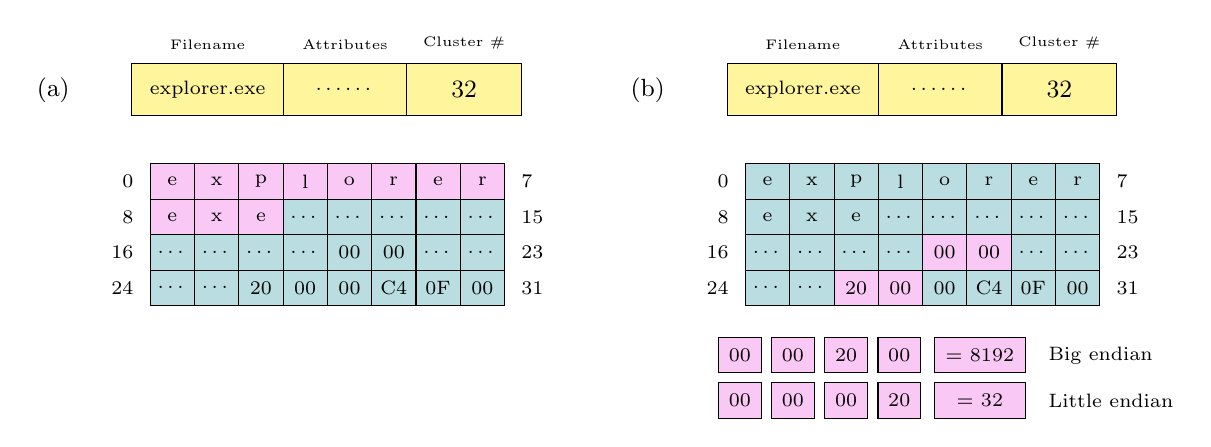
\begin{tikzpicture}[fatfig]
  \foreach \p/\dx/\hi in {a/0/{1,2,3,4,5,6,7,8,9,10,11}, b/420/{21,22,27,28}} {
    \begin{scope}[shift={(\dx,0)}]
      \node[font=\small, anchor=east] at (500,225) {(\p)};
      \fatent{537}{644}{731}{812}{206}{explorer.exe}{32}
      \foreach \v [count=\k] in {e,x,p,l,o,r,e,r, e,x,e,\dots,\dots,\dots,\dots,\dots,
                                  \dots,\dots,\dots,\dots,00,00,\dots,\dots, \dots,\dots,20,00,00,C4,0F,00} {
        \pgfmathtruncatemacro{\row}{(\k-1)/8}
        \pgfmathtruncatemacro{\col}{\k-1-8*\row}
        \draw[fill=freec] (550+31.25*\col,277+25*\row) rectangle ++(31.25,25);
      }
      \foreach \k in \hi {
        \pgfmathtruncatemacro{\row}{(\k-1)/8}
        \pgfmathtruncatemacro{\col}{\k-1-8*\row}
        \draw[fill=metac] (550+31.25*\col,277+25*\row) rectangle ++(31.25,25);
      }
      \foreach \v [count=\k] in {e,x,p,l,o,r,e,r, e,x,e,\dots,\dots,\dots,\dots,\dots,
                                  \dots,\dots,\dots,\dots,00,00,\dots,\dots, \dots,\dots,20,00,00,C4,0F,00} {
        \pgfmathtruncatemacro{\row}{(\k-1)/8}
        \pgfmathtruncatemacro{\col}{\k-1-8*\row}
        \node[font=\scriptsize] at (565.6+31.25*\col,289.5+25*\row) {\v};
      }
      \foreach \l/\r [count=\j from 0] in {0/7, 8/15, 16/23, 24/31} {
        \node[font=\scriptsize, anchor=east] at (545,289.5+25*\j) {\l};
        \node[font=\scriptsize, anchor=west] at (805,289.5+25*\j) {\r};
      }
    \end{scope}
  }
  \begin{scope}[shift={(420,0)}]
    \foreach \bytes/\val/\name [count=\j from 0] in {{00,00,20,00}/8192/Big endian, {00,00,00,20}/32/Little endian} {
      \foreach \b [count=\i from 0] in \bytes
        \node[draw, fill=metac, minimum width=5.4mm, minimum height=4.5mm, font=\scriptsize] at (546+37.5*\i,412+32*\j) {\b};
      \node[draw, fill=metac, minimum width=11.5mm, minimum height=4.5mm, font=\scriptsize, anchor=west] at (683,412+32*\j) {$=$ \val};
      \node[font=\scriptsize, anchor=west] at (757,412+32*\j) {\name};
    }
  \end{scope}
\end{tikzpicture}
\caption{The entry of \code{explorer.exe}: (a) bytes 0--10 hold the name; (b) bytes 20--21 and 26--27 hold the first cluster number, read big endian and little endian (after slides 129--132).}
\label{fig:fatdirbytes}
\end{figure}

\subsubsection{Long filenames}
In the old days, Uncle Bill set the rule that every file follows the 8.3 naming scheme. He later removed the constraint with a backward-compatible but super ugly design: \emph{LFN} (long filename) entries (\Cref{fig:lfn}).
\begin{itemize}
  \item The regular 8.3 entry is still there, so old systems keep working.
  \item In front of it come one or more LFN entries, each holding up to 13 characters of the long name in Unicode (2 bytes per character): 5 in bytes 1--10, 6 in bytes 14--25, and 2 in bytes 28--31.
  \item Byte 0 is a sequence number, and the sequence is upside down: LFN \#3, \#2, \#1, then the regular entry.
  \item Byte 11, the attribute byte, is always \code{0x0F} for an LFN entry, a combination that old systems ignore; byte 13 is a checksum of the 8.3 name, which ties the LFN entries to their regular entry.
\end{itemize}

\begin{figure}[H]
\centering
\begin{tikzpicture}[fatfig, x=0.17mm, y=-0.17mm]
  \node[font=\small, anchor=east] at (150,425) {(a)};
  \draw[fill=lfnc] (182,344) rectangle (418,376);
  \node[font=\scriptsize\bfseries, text=white] at (300,360) {Directory file};
  \foreach \t/\c [count=\i] in {LFN \#3/lfnrowc, LFN \#2/lfnrowl, LFN \#1/lfnrowc, Regular entry/lfnrowl} {
    \draw[fill=\c] (182,376+32.5*\i-32.5) rectangle (418,376+32.5*\i);
    \node[font=\scriptsize\ttfamily] at (300,376+32.5*\i-16.25) {\t};
  }
  \draw[sigc, thick] (420,378) -- (428,378) -- (428,471) -- (420,471);
  \draw[sigc, thick] (428,424.5) -- (436,424.5);
  \draw[sigc, thick, rounded corners=6pt] (447,375) rectangle (818,462);
  \fill[white] (449,413) -- (436,424.5) -- (449,436) -- cycle;
  \draw[sigc, thick] (448,413) -- (436,424.5) -- (448,436);
  \node[font=\scriptsize, align=left, text width=59mm, anchor=north west] at (452,380)
    {Each LFN entry represents up to 13 characters in Unicode (2~bytes per character).\\[2pt] Yet, the sequence is upside-down!};
  \draw[sigc, thick, rounded corners=6pt] (447,474) rectangle (818,505);
  \fill[white] (449,481) -- (420,489.5) -- (449,498) -- cycle;
  \draw[sigc, thick] (448,481) -- (420,489.5) -- (448,498);
  \node[font=\scriptsize, anchor=west] at (452,489.5) {The regular directory entry is still there.};
  \node[font=\small, anchor=east] at (150,630) {(b)};
  \node[anchor=north west, inner sep=0pt] at (182,522) {\scriptsize
    \begin{tabular}{|c|p{52mm}|}
      \hline
      \rowcolor{bootc}\textcolor{white}{\bfseries Bytes} & \multicolumn{1}{c|}{\cellcolor{bootc}\textcolor{white}{\bfseries Value (LFN directory entry)}} \\ \hline
      \rowcolor{rowc} 0 & Sequence Number. \\ \hline
      \rowcolor{metac} 1--10 & File name characters\newline (5 characters in Unicode). \\ \hline
      \rowcolor{rowc} 11 & File attributes --- \textcolor{sigc}{always 0x0F for LFN}. \\ \hline
      \rowcolor{rowc} 12 & Reserved. \\ \hline
      \rowcolor{rowc} 13 & Checksum. \\ \hline
      \rowcolor{metac} 14--25 & File name characters\newline (6 characters in Unicode). \\ \hline
      \rowcolor{rowc} 26--27 & Reserved. \\ \hline
      \rowcolor{metac} 28--31 & File name characters\newline (2 characters in Unicode). \\ \hline
    \end{tabular}};
\end{tikzpicture}
\caption{Long filenames: (a) LFN entries in front of the regular entry; (b) the layout of an LFN entry (after slides 133--134).}
\label{fig:lfn}
\end{figure}

\subsection{Reading a File}

\begin{enumerate}
  \item Read the first cluster number from the directory entry: \code{explorer.exe} starts at cluster 32.
  \item Look up the next cluster in the FAT, and read that cluster: FAT entry 32 holds 33.
  \item Repeat until an EOF entry is found in the FAT: entry 33 holds EOF, so the file is clusters 32 and 33. A FAT32 entry is EOF if its value is at least \code{0x0FFFFFF8}.
\end{enumerate}

\begin{figure}[H]
\centering
\begin{tikzpicture}[fatfig]
  % (a) step 1
  \node[font=\small, anchor=east] at (120,434) {(a)};
  \fatbar \cdrive
  \fatent{537}{644}{731}{812}{325}{explorer.exe}{32}
  \draw[arr] (755,362) .. controls (745,392) and (565,370) .. (550,399);
  % (b) step 2 and (c) step 3
  \foreach \p/\dy in {b/290, c/580} {
    \begin{scope}[shift={(0,\dy)}]
      \node[font=\small, anchor=east] at (120,434) {(\p)};
      \fatbar \cdrive
      \draw[dimarr] (293,220) -- node[above, font=\scriptsize] {32 bits} (400,220);
      \fatcol{293}{236}{107}{EOF, \dots, 33, EOF, 0}
      \fatent{537}{644}{731}{812}{325}{explorer.exe}{32}
      \draw[{Stealth[length=1.4mm]}-{Stealth[length=1.4mm]}, densely dotted] (357,366) -- (362,402);
      \draw[{Stealth[length=1.4mm]}-{Stealth[length=1.4mm]}, densely dotted] (397,366) -- (430,402);
    \end{scope}
  }
  \begin{scope}[shift={(0,290)}]
    \draw[hl] (325,288) rectangle (369,310);
    \draw[arr] (755,362) .. controls (745,400) and (500,400) .. (487,370) .. controls (478,330) and (450,300) .. (403,298.5);
  \end{scope}
  \begin{scope}[shift={(0,580)}]
    \node[hl, fit=(fi4), inner sep=1pt] {};
    \draw[arr] (755,362) .. controls (745,400) and (500,400) .. (487,370) .. controls (478,345) and (450,323) .. (403,323.5);
    \node[callout, rounded corners=0pt, anchor=west] (eof) at (425,281) {EOF $\geqslant$ \texttt{0x0ffffff8}};
    \fill[white] (437,290) -- (402,323) -- (455,290) -- cycle;
    \draw (437,291) -- (402,323) -- (455,291);
  \end{scope}
\end{tikzpicture}
\caption{Reading \code{explorer.exe}: (a) the first cluster comes from the directory entry; (b) the FAT gives the next cluster; (c) until an EOF entry is found (after slides 135--137).}
\label{fig:fatread}
\end{figure}

Two notes. The kernel usually needs to know all the cluster numbers before the actual reading starts, so a file is not necessarily read sequentially. And besides EOF, unallocated ($0$), and allocated, a cluster can also be \emph{damaged}, i.e., contain bad sectors; the FAT value of a damaged cluster is \code{0x0FFFFFF7}.

\subsection{Writing a File}

To append one cluster to \code{explorer.exe} (\Cref{fig:fatwrite}):
\begin{enumerate}
  \item Locate the cluster at the end of the file by following the chain: cluster 33.
  \item Look up the \emph{FSINFO} structure, in the reserved area, to find the next free cluster: 34. (The location of FSINFO is written in the boot sector; FSINFO is where FAT32 keeps the two hints of \Cref{fig:fathints}.)
  \item Allocate the cluster by changing the FATs and FSINFO: entry 33 becomes 34, entry 34 becomes EOF, the number of free clusters drops from 100 to 99, and the next free cluster becomes 35. \emph{Both} FATs must be updated.
\end{enumerate}

\begin{figure}[H]
\centering
\begin{tikzpicture}[fatfig]
  \foreach \p/\dy in {a/0, b/300} {
    \begin{scope}[shift={(0,\dy)}]
      \node[font=\small, anchor=east] at (120,434) {(\p)};
      \fatbar \cdrive
      \node[font=\scriptsize] at (318,268) {FSINFO structure};
      \node[font=\tiny, align=left, anchor=north west] at (215,350) {inside the\\ reserved space};
      \draw[-{Stealth[length=1.4mm]}, densely dotted] (331,350) -- (331,398);
    \end{scope}
  }
  % (a) steps 1 and 2
  \fsinfo{218}{287}{150}{100}{34}
  \fatcol{575}{234}{106}{EOF, \dots, 33, EOF, 0, 0}
  \fatblock{fc3}{1} \fatblock{fc4}{2}
  \node[hl, fit=(fi4), inner sep=0pt] {};
  \node[hl, fit=(fi5), inner sep=0pt] (n34) {};
  \draw[-{Stealth[length=1.4mm]}, densely dotted] (425,325) -- (n34.west);
  % (b) step 3
  \begin{scope}[shift={(0,300)}]
    \fsinfo{218}{287}{150}{99}{35}
    \fatcol{575}{234}{106}{EOF, \dots, 33, 34, EOF, 0}
    \fatblock{fc3}{1} \fatblock{fc4}{2} \fatblock{fc5}{3}
    \draw[hl] (372,281) rectangle (414,343);
    \draw[hl] (605,309) rectangle (651,359);
    \node[hl, fit=(fi6), inner sep=1pt] (n35) {};
    \draw[-{Stealth[length=1.4mm]}, densely dotted] (425,333) -- (n35.west);
    \node[draw, font=\tiny, anchor=north west] at (706,212) {Both FATs must be updated.};
  \end{scope}
\end{tikzpicture}
\caption{Appending a cluster to a file that ends at cluster 33: (a) find the end of the chain and the next free cluster in FSINFO; (b) two FAT entries and both FSINFO fields change (after slides 139--141).}
\label{fig:fatwrite}
\end{figure}

If more than one extra cluster is needed, a circular, next-available search is performed to find each further unallocated cluster. Even after the writing finishes, the kernel still searches for one more unallocated cluster, so that the ``next free cluster'' hint in FSINFO again names a free cluster.

\subsection{Deleting a File}

To delete \code{explorer.exe}, now clusters 32, 33, and 34 (\Cref{fig:fatdelete}):
\begin{enumerate}
  \item Find the directory entry and, from it and the FAT, the locations of the clusters.
  \item Set all the next-cluster fields of that file in the FATs to $0$.
  \item Update the FSINFO structure: the number of free clusters goes from 99 to 102, and the next free cluster becomes 32.
  \item Change the first character of the filename to \code{0xE5}, which marks the entry as unallocated (\code{explorer.exe} becomes \code{\aa xplorer.exe} when \code{0xE5} is shown as a character).
\end{enumerate}

\begin{figure}[H]
\centering
\begin{tikzpicture}[fatfig]
  \foreach \p/\dy in {a/0, b/290} {
    \begin{scope}[shift={(0,\dy)}]
      \node[font=\small, anchor=east] at (120,434) {(\p)};
      \fatbar \cdrive
      \node[font=\scriptsize, anchor=east] at (264,344) {FSINFO structure};
    \end{scope}
  }
  % (a) step 1
  \fatent{206}{313}{400}{469}{244}{explorer.exe}{32}
  \fsinfo{270}{319}{150}{99}{35}
  \fatcol{575}{234}{106}{EOF, \dots, 33, 34, EOF, 0}
  \fatblock{fc3}{1} \fatblock{fc4}{2} \fatblock{fc5}{3}
  % (b) steps 2 to 4
  \begin{scope}[shift={(0,290)}]
    \fatent{206}{313}{400}{469}{244}{\aa xplorer.exe}{32}
    \node[hl, fit=(en), inner sep=0pt] {};
    \fsinfo{270}{319}{150}{102}{32}
    \draw[hl] (424,313) rectangle (464,375);
    \fatcol{575}{234}{106}{EOF, \dots, 0, 0, 0, 0}
    \draw[hl] (605,284) rectangle (651,359);
  \end{scope}
\end{tikzpicture}
\caption{Deleting \code{explorer.exe}: (a) the entry, FSINFO, and the chain 32, 33, 34; (b) the chain is zeroed, FSINFO is updated, and the first character becomes \code{0xE5} (after slides 143--146).}
\label{fig:fatdelete}
\end{figure}

\begin{keypoint}[Lazy Deletion]
  The file is not really deleted. Neither the clusters nor most of the directory entry are erased, so a search of the free space finds all deleted file contents, and they persist until the deallocated clusters are reused. This is a trade-off between performance (during deletion) and security.
\end{keypoint}

How to delete a file securely is a topic of its own (the slides point to \emph{Remembrance of Data Passed: A Study of Disk Sanitization Practices}). Conversely, how to recover a deleted file?
\begin{itemize}
  \item If you really care about the file, \emph{pull the power plug immediately}, which prevents its clusters from being overwritten. (Sorry, laptop users.)
  \item If the file is no larger than one cluster, recovery is easy: the first cluster number is still in the directory entry. (Only the first character of the name is lost, so other files with the same suffix may also turn up.)
  \item If it is larger than one cluster, the addresses of the other clusters are gone, since the FAT chain was zeroed. But because of the next-available search, the clusters of a file are likely to have been allocated contiguously. If not, you had better know the exact file size and checksum of the deleted file beforehand, so that you can recover it by brute force.
\end{itemize}

\enlargethispage{\baselineskip}
\subsection{Summary}

FAT is a simple yet pretty good file system. Its space overhead is 4 bytes (one FAT entry) per data cluster. Security is not a consideration in its design: it keeps no owners or permissions, and it deletes lazily. It was widely deployed, and it still is: it dominates SD cards and USB flash drives because every OS can read it.

\section{ext2/3/4 in Action}
\label{sec:ext}

\subsection{Facts About ext4}

The primary file system on Linux is \emph{ext4}, the fourth extended file system. Its default block size is 4\,KB (configurable from 1\,KB to 64\,KB), and its default block address is 32 bits, configurable to 64. Most of what follows holds for ext2 and ext3 as well.

\subsection{Block Groups}

\begin{definition}[Block Group]
  An ext2/3/4 file system is partitioned into \emph{block groups} with the same internal structure: a block bitmap, an inode bitmap, an inode table, and the file content of that group. The \emph{group descriptor table} (GDT), stored after the superblock, records for each group where its block bitmap, inode bitmap, and inode table start.
\end{definition}

\begin{figure}[htbp]
\centering
\begin{tikzpicture}[x=1cm]
  \draw[fill=bootc] (0,0) rectangle (1.0,0.7); \node[font=\scriptsize, text=white, align=center] at (0.5,0.35) {Super-\\ block};
  \draw[fill=datac] (1.0,0) rectangle (1.4,0.7);
  \foreach \g in {0,...,3} { \draw[fill=freec] (1.4+1.6*\g,0) rectangle ++(1.6,0.7); \node[font=\scriptsize] at (2.2+1.6*\g,0.35) {Group \g}; }
  \draw[fill=rowc] (3.0,1.4) rectangle (4.0,2.1); \node[font=\tiny, align=center] at (3.5,1.75) {block\\ bitmap};
  \draw[fill=rowc] (4.0,1.4) rectangle (5.0,2.1); \node[font=\tiny, align=center] at (4.5,1.75) {inode\\ bitmap};
  \draw[fill=metac] (5.0,1.4) rectangle (6.0,2.1); \node[font=\tiny, align=center] at (5.5,1.75) {inode\\ table};
  \draw[fill=usedc] (6.0,1.4) rectangle (7.2,2.1); \node[font=\tiny, align=center] at (6.6,1.75) {file\\ content};
  \draw[densely dotted] (3.0,1.4) -- (3.0,0.7); \draw[densely dotted] (7.2,1.4) -- (4.6,0.7);
  \draw[arr] (0.4,1.5) node[above, font=\scriptsize] {group descriptor table} -- (1.2,0.7);
\end{tikzpicture}
\caption{An ext2/3/4 file system: the superblock and the group descriptor table, then block groups that all share one internal structure (after slide 152).}
\label{fig:blockgroups}
\end{figure}

Why do this? For performance and reliability. Keeping the metadata of a group close to the file contents of the same group means the disk head does not have to travel a long distance between an inode and its data. And the metadata is scattered over the disk, so there is no single point of failure. (ext2/3/4 keep backup copies of the superblock and the GDT in some of the groups.)

\begin{example}[Reading the Superblock]
  \code{tune2fs -l} prints the superblock:
\begin{lstlisting}[style=sh]
# tune2fs -l /dev/sda1
Filesystem OS type:       Linux
Inode count:              122624
Block count:              244983
Reserved block count:     12249
Free blocks:              228306
Free inodes:              122586
First block:              0
Block size:               4096
Blocks per group:         32768
Fragments per group:      32768
Inodes per group:         15328
Inode blocks per group:   479
First inode:              11
Inode size:               128
Journal inode:            8
First orphan inode:       27
\end{lstlisting}
  The first group of lines is general file system information, the second describes the layout, and the third the inode usage. The numbers are consistent: $244\,983$ blocks at $32\,768$ per group make 8 groups, and $8 \times 15\,328 = 122\,624$ inodes; $15\,328$ inodes of 128 bytes fill $15\,328 \times 128 / 4096 = 479$ blocks per group.
\end{example}

\subsection{The Metadata Structures}

For simplicity, consider a single block group from now on (\Cref{fig:extlayout}).
\begin{itemize}
  \item The \emph{block bitmap} stores the allocation status of the blocks of the group.
  \item The \emph{inode bitmap} stores the allocation status of the inodes of the group.
  \item The \emph{inode table} stores the contents of all the inodes of the group. Every inode has the same size, specified in the superblock, and the inodes are stored sequentially.
\end{itemize}

\begin{figure}[htbp]
\centering
\begin{tikzpicture}[x=1cm]
  \draw[fill=bootc] (0,0) rectangle (1.0,0.7); \node[font=\scriptsize, text=white, align=center] at (0.5,0.35) {Super-\\ block};
  \draw[fill=rowc] (1.0,0) rectangle (1.9,0.7); \node[font=\tiny, align=center] at (1.45,0.35) {block\\ bitmap};
  \draw[fill=rowc] (1.9,0) rectangle (2.8,0.7); \node[font=\tiny, align=center] at (2.35,0.35) {inode\\ bitmap};
  \draw[fill=metac] (2.8,0) rectangle (4.8,0.7); \node[font=\scriptsize] at (3.8,0.35) {Inode table};
  \foreach \k [count=\j] in {2,1,1,0,1,0,0,1,1,1,0,2,0,1,1,0,0,1,1,0,1,1,0,0,1} {
    \pgfmathsetmacro{\xx}{4.8+0.22*(\j-1)}
    \ifnum\k=1 \draw[fill=usedc] (\xx,0) rectangle ++(0.22,0.7);
    \else\ifnum\k=2 \draw[fill=dirc] (\xx,0) rectangle ++(0.22,0.7);
    \else \draw[fill=freec] (\xx,0) rectangle ++(0.22,0.7); \fi\fi
  }
  \node[font=\scriptsize\ttfamily, anchor=south] at (2.35,0.75) {1110010\dots};
  \foreach \i/\t in {0/1,1/2,2/3,3/\dots,4/100} \node[cell, fill=metac, minimum width=9mm] at (3.4+0.9*\i,-0.9) {\t};
  \draw[densely dotted] (2.8,0) -- (2.95,-0.65); \draw[densely dotted] (4.8,0) -- (7.45,-0.65);
  \foreach \i in {0,1,4} \draw[{Stealth[length=1.2mm]}-{Stealth[length=1.2mm]}] (2.95+0.9*\i,-1.3) -- node[below, font=\tiny] {128 B} (3.85+0.9*\i,-1.3);
\end{tikzpicture}
\caption{One block group: the bitmaps, and an inode table of fixed-size 128-byte inodes numbered from 1 (after slides 155--156).}
\label{fig:extlayout}
\end{figure}

\subsubsection{The inode}
An ext2 inode is a 128-byte structure (\Cref{tab:inode}); compare it with \code{struct stat} in \Cref{sec:files}, which is mostly a copy of it. Because inodes are fixed-size, the start of inode $i$ is at byte
\[
  \text{start of the inode table} + (i - 1) \times 128.
\]

\begin{table}[htbp]
\centering
\small
\begin{tabular}{rl}
  \toprule
  Bytes & Value \\
  \midrule
  0--1 & file type and permission \\
  2--3 & user ID \\
  4--7 & lower 32 bits of the file size in bytes \\
  8--23 & time information \\
  24--25 & group ID \\
  26--27 & link count \\
  \dots & \dots \\
  40--87 & 12 direct data block pointers \\
  88--91 & single indirect block pointer \\
  92--95 & double indirect block pointer \\
  96--99 & triple indirect block pointer \\
  \dots & \dots \\
  108--111 & upper 32 bits of the file size in bytes \\
  \bottomrule
\end{tabular}
\caption{The 128-byte ext2 inode. The 15 block pointers are those of \Cref{fig:indirect} (after slide 156).}
\label{tab:inode}
\end{table}

\begin{definition}[Special Inodes]
  Inodes are numbered from 1; there is no inode 0. The first 10 inodes are reserved for special purposes: inode 1 always points to the bad blocks, inode 2 always points to the \emph{root directory}, and inode 8 usually points to the journal's data blocks (\Cref{sec:recovery}). That is why the superblock above says ``First inode: 11''.
\end{definition}

Inode 2 answers the question left open in \Cref{sec:fsmeta}: in ext2/3/4, the root directory is found by reading a fixed inode.

\subsection{Directory Entries}

A directory is stored in data blocks, and it always contains at least two entries: \code{.} and \code{..}. Each directory entry has four fields: the inode number (4 bytes), the entry length (2 bytes), the name length (2 bytes), and the filename (up to 255 bytes).

\begin{center}
\small
\begin{tabular}{rrrl}
  \toprule
  Inode \# & Entry length & Name length & Filename \\
  \midrule
  123 & 12 & 2 & \code{.} \\
  2 & 12 & 3 & \code{..} \\
  5\,086 & 16 & 7 & \code{12.jpg} \\
  \bottomrule
\end{tabular}
\end{center}

Why is the entry of \code{12.jpg} 16 bytes long, not $4 + 2 + 2 + 7 = 15$? Two reasons. The name length counts the terminating \code{'\textbackslash 0'}, which is why the 6-character name \code{12.jpg} has length 7 and \code{.} has length 2. And entries are padded for byte alignment to a multiple of 4 bytes, so $15$ rounds up to $16$ (and $10$, for \code{.}, to $12$). Because the entry length is stored explicitly, an entry can also be \emph{longer} than its name requires; deletion uses that (below).

\begin{remark}
  This is the slides' model. The actual ext2 on-disk entry splits the 2-byte name-length field into a 1-byte name length and a 1-byte file type, and does not store the terminating \code{'\textbackslash 0'}; the padding to a multiple of 4 is the same. Check the ext2 documentation if the details matter.
\end{remark}

\subsection{Hard Links}

\begin{definition}[Hard Link]
  A \emph{hard link} is a directory entry pointing to an existing file, i.e., to an existing inode. No new file content and no new inode are created.
\end{definition}

\begin{example}[Making a Hard Link]
\begin{lstlisting}[style=sh]
# ls /dir1/12.jpg
12.jpg
# ln /dir1/12.jpg /my_link
\end{lstlisting}
  A new directory entry \code{my\_link} with inode number 5086 is added to \code{/} (\Cref{fig:hardlink}). Conceptually, this creates one file with two filenames. Deleting one of the two directory entries does not delete the file content.
\end{example}

\begin{figure}[htbp]
\centering
\begin{tikzpicture}
  \dirtab{d}{0cm}{Directory: \code{/dir1}}{123/., 2/.., 5{,}086/12.jpg}
  \dirtab{r}{5.2cm}{Directory: \code{/}}{2/., 2/.., 5{,}086/my\_link}
  \node[cell, fill=usedc, minimum width=18mm, font=\scriptsize\bfseries] (ino) at (3.6,-2.6) {inode 5086};
  \node[cell, fill=bootc, text=white, minimum width=18mm, below=0pt of ino, font=\tiny\bfseries] {link count $= 2$};
  \draw[arr] (d-n3.south) |- (ino.west);
  \draw[arr] (r-n3.south) |- (ino.east);
\end{tikzpicture}
\caption{After \code{ln /dir1/12.jpg /my\_link}, two directory entries in two directories refer to the same inode, whose link count is 2 (after slides 159--161).}
\label{fig:hardlink}
\end{figure}

\begin{keypoint}[Link Count]
  The \emph{link count} field of the inode keeps track of how many directory entries point to the file. Removing a link with the \code{unlink()} system call (which is what \code{rm} calls) decrements it by 1. Only when the link count becomes 0 is the file content removed: its data blocks and its inode.
\end{keypoint}

In \Cref{fig:hardlink}, \code{rm /my\_link} brings the link count of inode 5086 from 2 to 1 and leaves the file intact; a subsequent \code{rm /dir1/12.jpg} brings it to 0, and the file is deleted.

\subsubsection{Directories and their link counts}
Two hard links are special: the entry \code{.} of a directory is a hard link to the directory itself, and \code{..} is a hard link to its parent. Hence:
\begin{itemize}
  \item When a regular file is created, its link count is always 1 (its entry in the parent).
  \item When a directory is created, its link count is always 2: its entry in the parent, and its own \code{.} (\Cref{fig:dirlinks}). Each subdirectory created inside it later adds 1, through the subdirectory's \code{..}.
\end{itemize}
\begin{lstlisting}[style=sh]
# stat /boot/grub/menu.lst
  File: `/boot/grub/menu.lst'
  Size: 4552        Blocks: 16         IO Block: 4096   regular file
Device: 801h/2049d  Inode: 30669       Links: 1
# mkdir temp
# stat temp
  File: `temp'
  Size: 4096        Blocks: 8          IO Block: 4096   directory
Device: 804h/2052d  Inode: 10994310    Links: 2
\end{lstlisting}

\begin{figure}[htbp]
\centering
\begin{tikzpicture}
  \dirtab{p}{0cm}{Parent of \code{temp}}{123/., 2/.., 10{,}994{,}310/temp}
  \dirtab{q}{5.6cm}{The new directory \code{temp}}{10{,}994{,}310/., 123/..}
  \draw[arr, densely dashed] (p-f3.east) to[out=0, in=180] node[below right, font=\scriptsize] {link} (q-n1.west);
  \draw[arr, densely dashed] (q-f1.east) to[out=0, in=0, looseness=2] node[right, font=\scriptsize] {link} (q-f1.south east);
\end{tikzpicture}
\caption{A new directory has two links: its entry in the parent, and its own entry \code{.}; its \code{..} adds a link to the parent (after slide 164).}
\label{fig:dirlinks}
\end{figure}

\begin{example}[The Link Count of the Root]
\begin{lstlisting}[style=sh]
# ls -F /
bin/    dev/   initrd/          lib/         mnt/   root/  sys/  var/
boot/   etc/   initrd.img@      lost+found/  opt/   sbin/  tmp/  vmlinuz@
cdrom@  home/  initrd.img.old@  media/       proc/  srv/   usr/  vmlinuz.old@
# stat /
  File: `/'
  Size: 4096          Blocks: 8          IO Block: 4096   directory
Device: 802h/2050d    Inode: 2           Links: 21
\end{lstlisting}
  The root is inode 2, as promised. It has 19 subdirectories (the entries marked \code{/}; those marked \code{@} are symbolic links and do not count). Its 21 links are the \code{..} of the 19 subdirectories, plus its own \code{.}, plus its own \code{..}, since the parent of \code{/} is \code{/} itself.
\end{example}

Removing an (empty) directory with \code{rmdir()} is therefore as simple as removing its directory entry from the parent and decrementing the link counts.

\subsection{Symbolic Links}

\begin{definition}[Symbolic Link]
  A \emph{symbolic link} is a file of its own, whose content is the pathname of its target. Unlike a hard link, a new inode is created for it.
\end{definition}

\begin{lstlisting}[style=sh]
# ln -s /dir1/12.jpg /my_link
# ls -l /my_link
/my_link -> /dir1/12.jpg
\end{lstlisting}
The new entry \code{my\_link} in \code{/} now has its own inode, 6120, rather than 5086. Since it stores a path and not an inode number, a symbolic link can cross file systems and can point to a directory, but it dangles if the target is removed.

Where is the target path stored? It depends on its length. A path shorter than 60 characters is stored right inside the inode, in the space of the 12 direct and 3 indirect block pointers: $(12 + 3) \times 4 = 60$ bytes. A longer path gets a data block of its own.

\subsection{Creating a File}

Creating \code{/dir1/hello.txt} takes six steps.
\begin{enumerate}
  \item Use a linear search in the inode bitmap to find an unallocated inode for the new file: inode 1024.
  \item Use a linear search in the block bitmap to find unallocated data blocks for it.
  \item Read the inode of the root directory, inode 2.
  \item Following its data block pointers, read the directory entries of \code{/}, and find \code{dir1}: inode 123.
  \item Read inode 123 and its data blocks, and construct the directory entries of \code{/dir1}: \code{.}, \code{..}, \code{panic.c} (inode 456, length 16), \code{picture.jpg} (inode 894, length 20).
  \item Add a new directory entry \code{hello.txt} with inode 1024 to \code{/dir1}.
\end{enumerate}

\subsection{Deleting a File}

Deleting \code{/dir1/picture.jpg}:
\begin{enumerate}
  \item Read the inode and the data blocks of \code{/dir1}, and locate the inode of \code{picture.jpg}: 894.
  \item Read inode 894 and decrement its link count. It becomes 0.
  \item Deallocate the data blocks and the inode by resetting the corresponding bits in the block bitmap and the inode bitmap.
  \item Change the entry length of the directory entry \emph{before} \code{picture.jpg}: the new length of \code{panic.c} is its original length plus that of \code{picture.jpg}, $16 + 20 = 36$.
\end{enumerate}

\begin{center}
\small
\begin{tabular}{rrl@{\qquad}rrl}
  \toprule
  \multicolumn{3}{c}{Before} & \multicolumn{3}{c}{After} \\
  Inode \# & Length & Filename & Inode \# & Length & Filename \\
  \midrule
  123 & 12 & \code{.} & 123 & 12 & \code{.} \\
  2 & 12 & \code{..} & 2 & 12 & \code{..} \\
  456 & 16 & \code{panic.c} & 456 & \textcolor{sigc}{36} & \code{panic.c} \\
  894 & 20 & \code{picture.jpg} & \textcolor{cmt}{894} & \textcolor{cmt}{20} & \textcolor{cmt}{\code{picture.jpg}} \\
  1024 & 20 & \code{hello.txt} & 1024 & 20 & \code{hello.txt} \\
  \bottomrule
\end{tabular}
\end{center}

The change of the entry length makes a traversal of the directory jump from \code{panic.c} straight to \code{hello.txt}, skipping the deleted entry. This leaves holes among the directory entries, so when a new file is created in the directory, the FS should check whether some hole is large enough for the new entry.

\begin{keypoint}
  As in FAT32, the file is not actually deleted: its entry is skipped, and its bits are cleared, but its data blocks are not erased. In ext2 even the data block pointers in the inode remain; in ext3 and ext4 they are removed, which makes recovery much harder.
\end{keypoint}

\section{Linux File System Internals}
\label{sec:vfs}

% Figure palette for this section, after the slides' kernel-structure diagrams
\definecolor{vpind}{HTML}{353598}   % struct files_struct
\definecolor{vpyel}{HTML}{FFFF66}   % NTFS functions
\tikzset{
  vpts/.style={draw=white, very thick, rounded corners=6pt, fill=datac},
  vpfs/.style={draw=white, very thick, rounded corners=5pt, fill=vpind},
  vpw/.style={draw=white, thick, text=white, font=\scriptsize, inner sep=2pt, minimum height=4.5mm},
  vpslot/.style={draw=white, fill=dirc, font=\scriptsize, minimum size=4.5mm, inner sep=0pt},
  vpsq/.style={draw=white, fill=dirc, minimum size=4mm, inner sep=0pt},
  vpmod/.style={fill=metac, font=\scriptsize\bfseries, align=center, inner sep=3pt},
  vpkern/.style={fill=kspace, rounded corners=3pt, inner sep=8pt,
                 label={[font=\small\itshape, anchor=south west, xshift=3pt, yshift=3pt]south west:Kernel memory}},
  vpdot/.style={-{Stealth[length=1.6mm]}, densely dotted, thick},
  % a stack of platters with "Disk" on top; anchors -top, -bot, -west, -east
  pics/vpdisk/.style={code={
    \foreach \y in {-0.6,-0.45,-0.3,-0.15,0} {
      \fill[black!45, draw=white, line width=0.8pt] (-0.62,\y+0.15) -- (-0.62,\y)
        arc[start angle=180, end angle=360, x radius=0.62, y radius=0.16] -- (0.62,\y+0.15) -- cycle;
    }
    \fill[black!45, draw=white, line width=0.8pt] (0,0.15) ellipse[x radius=0.62, y radius=0.16];
    \node[text=white, font=\scriptsize\bfseries] at (0,0.15) {Disk};
    \coordinate (-top) at (0,0.31); \coordinate (-bot) at (0,-0.76);
    \coordinate (-west) at (-0.62,-0.2); \coordinate (-east) at (0.62,-0.2);
  }},
  % a file: a page with a few text lines; anchors -west, -south
  pics/vpdoc/.style={code={
    \draw[fill=freec] (-0.4,-0.45) rectangle (0.4,0.45);
    \foreach \a/\b/\y in {-0.28/0.2/0.3, -0.1/0.3/0.13, -0.28/0.2/-0.04, -0.18/0.3/-0.25}
      \draw[thin] (\a,\y) -- (\b,\y);
    \coordinate (-west) at (-0.4,0); \coordinate (-south) at (0,-0.45);
  }},
  % \vptab: a VFS function structure, four orange rows
  pics/vptab/.style={code={
    \foreach \k in {0,...,3} \draw[white, fill=dirc] (0,-0.17*\k) rectangle (0.65,-0.17*\k-0.17);
    \foreach \k in {0,...,3} \coordinate (-r\k) at (0.65,-0.17*\k-0.085);
    \coordinate (-nw) at (0,0); \coordinate (-sw) at (0,-0.68);
    \coordinate (-ne) at (0.65,0); \coordinate (-se) at (0.65,-0.68);
  }},
}

The previous sections were about the file organization level of \Cref{sec:alloc}. This one moves up to the logical representation level: how the kernel models a file. It faces two ways: toward the user program it speaks in file descriptors and file content; toward the disk, in metadata and file content (\Cref{fig:logiclevel}).

\begin{figure}[H]
\centering
\begin{tikzpicture}
  \node[draw=usedc!60!black, fill=usedc, font=\scriptsize\bfseries, minimum width=20mm, minimum height=7mm] (user) at (0,0) {User program};
  \node[draw=bootc, fill=kspace, font=\scriptsize\bfseries, minimum width=20mm, minimum height=7mm] (kern) at (4.6,0) {Kernel};
  \pic (dk) at (8.2,0.15) {vpdisk};
  \draw[{Stealth[length=2mm]}-{Stealth[length=2mm]}, thick] (user) -- node[above, font=\scriptsize, align=center] {File descriptor and\\ file content} (kern);
  \draw[{Stealth[length=2mm]}-{Stealth[length=2mm]}, thick] (kern) -- node[above, font=\scriptsize, align=center] {Metadata and\\ file content} (dk-west |- kern);
\end{tikzpicture}
\caption{The logical representation level: the kernel between the user program and the disk (after slide 181).}
\label{fig:logiclevel}
\end{figure}

\subsection{From File Descriptor to Inode}

\begin{lstlisting}
int fd;
fd = open("/dev/zero", O_RDONLY);   // a file descriptor, if the call succeeds
\end{lstlisting}
A user program is given a file descriptor as the abstract representation of an open file. It is so abstract that it is just a number. What does the number mean?

There is a strong relationship between a process and its open files: each process has its own set of them, managed inside its \ts{} (\Cref{sec:kernel}). The chain of structures is as follows (\Cref{fig:openfile}).
\begin{itemize}
  \item The \ts{} has a pointer \code{*files} to a \code{struct files\_struct}, which manages all the open files of the process: an array \code{fd} of open files, and \code{next\_fd}, the next descriptor to hand out. By default every process starts with three open files: descriptor 0 for \code{stdin}, 1 for \code{stdout}, and 2 for \code{stderr}.
  \item When the process calls \code{open()}, the \emph{file system module} reads the file's metadata from the disk: the directory entry (with the inode number), the block addresses, and so on.
  \item The open file is represented as a \code{struct file} and added to the process. A new file descriptor, here 3, is allocated for it: the descriptor is the index of that \code{struct file} in the \code{fd} array.
  \item The \code{struct file} refers to the \emph{directory entry} of the file, which in turn contains the name and the inode of the file.
\end{itemize}

\begin{figure}[H]
\centering
\begin{tikzpicture}
  % (a) task_struct -> files_struct -> fd array; the FS module reads the disk
  \node[font=\small, anchor=east] at (-0.45,-1.2) {(a)};
  \node[vpts, minimum width=25mm, minimum height=22mm, anchor=north west] (ts) at (0,0) {};
  \node[font=\scriptsize\bfseries, text=white] at (1.25,-0.3) {struct task\_struct};
  \node[vpw] at (0.55,-0.95) {pid}; \node[vpw] at (1.6,-0.95) {counter};
  \node[vpw] (files) at (1.8,-1.75) {*files};
  \node[vpfs, minimum width=16mm, minimum height=18.5mm, anchor=north west] (fs) at (3.2,-0.35) {};
  \node[font=\scriptsize\bfseries, text=white, align=center] at (4.0,-0.75) {struct\\[-2pt] files\_struct};
  \node[vpw] at (4.0,-1.3) {next\_fd};
  \node[vpw] (fdarr) at (4.0,-1.75) {fd};
  \draw[arr] (files.east) -- (fs.west |- files);
  \foreach \k in {0,...,3} \node[vpslot] (s\k) at (5.3+0.6*\k,-1.75) {\k};
  \draw[arr] (fdarr.east) -- (s0.west);
  \foreach \k [evaluate=\k as \j using int(\k+1)] in {0,1,2} \draw[-{Stealth[length=1.3mm]}, thick] (s\k.east) -- (s\j.west);
  \node[vpmod] (mod) at (7.1,-0.6) {File system\\ module};
  \draw[arr] (mod.south -| s3) -- (s3.north);
  \node[font=\scriptsize, anchor=south west] (c1) at (2.7,0.05) {Manages all the opened files};
  \draw[vpdot] (c1.south west) ++(0.2,0) -- (files.north east);
  \node[font=\scriptsize] (c2) at (6.45,-2.55) {A list of opened files};
  \draw[vpdot] (c2.north) ++(-0.4,0) -- (s1.south);
  \begin{scope}[on background layer]
    \node[vpkern, fit={(ts)(fs)(mod)(c1)(c2)}] {};
  \end{scope}
  \pic (dk) at (8.75,-1.3) {vpdisk};
  \draw[arr] (mod.east) to[out=0, in=90] (dk-top);
  % (b) struct file -> directory entry -> the file on disk
  \begin{scope}[yshift=-3.6cm]
    \node[font=\small, anchor=east] at (-0.45,-1.2) {(b)};
    \node[vpts, fill=dirc, minimum width=26mm, minimum height=22mm, anchor=north west] (sf) at (0,0) {};
    \node[font=\small\bfseries, text=white] at (1.3,-0.35) {struct file};
    \node[vpw] (de) at (1.3,-1.1) {directory entry};
    \node[font=\scriptsize\bfseries, text=white] at (1.3,-1.7) {\dots\dots};
    \node[draw, fill=freec, rounded corners=5pt, minimum width=14mm, minimum height=16mm, anchor=north west] (dent) at (3.6,-0.5) {};
    \node[draw, font=\scriptsize, inner sep=2pt, minimum height=4mm] at (4.3,-0.82) {name};
    \node[draw, font=\scriptsize, inner sep=2pt, minimum height=4mm] (ino) at (4.3,-1.38) {inode};
    \node[font=\scriptsize\bfseries] at (4.3,-1.8) {\dots};
    \draw[arr] (de.east) -- (dent.west |- de);
    \coordinate (kr) at (6.0,0);
    \coordinate (kb) at (0,-2.55);
    \begin{scope}[on background layer]
      \node[vpkern, fit={(sf)(dent)(kr)(kb)}] {};
    \end{scope}
    \pic (doc) at (7.5,-0.45) {vpdoc};
    \pic (dk2) at (7.6,-2.0) {vpdisk};
    \draw[vpdot] (dent.east |- ino) to[out=0, in=180] (doc-west);
    \draw[vpdot] (doc-south) -- (dk2-top);
  \end{scope}
\end{tikzpicture}
\caption{An open file in the Linux kernel. (a) The \ts{} points to the \code{files\_struct}, whose \code{fd} array lists the open files; on \code{open()}, the file system module reads the metadata from the disk and the new file gets descriptor 3. (b) The \code{struct file} refers to the directory entry, which holds the name and the inode of the file (after slides 183--187).}
\label{fig:openfile}
\end{figure}

\begin{keypoint}[Scope of a File Descriptor]
  The scope of a file descriptor is restricted to its process. Different processes may use different descriptors to refer to the same file, and the same descriptor number in two processes may refer to different files (\Cref{fig:fdscope}).
\end{keypoint}

\begin{figure}[H]
\centering
\begin{tikzpicture}
  \foreach \r/\dx/\dy in {1/0/0, 2/0.45/-1.5} {
    \begin{scope}[xshift=\dx cm, yshift=\dy cm]
      \node[vpts, minimum width=13mm, minimum height=13mm] (t\r) at (0.8,-0.85) {};
      \node[vpfs, minimum width=9.5mm, minimum height=8.5mm] (f\r) at (2.35,-1.05) {};
      \foreach \k in {0,1,2} \node[vpsq] (q\r\k) at (3.45+0.55*\k,-1.05) {};
      \node[font=\scriptsize\bfseries] at (5.05,-1.05) {\dots};
      \draw[arr] (t\r.east |- f\r) -- (f\r.west);
      \draw[arr] (f\r.center) -- (q\r0.west);
      \draw[-{Stealth[length=1.3mm]}, thick] (q\r0) -- (q\r1);
      \draw[-{Stealth[length=1.3mm]}, thick] (q\r1) -- (q\r2);
    \end{scope}
  }
  \coordinate (kr) at (6.0,0); \coordinate (kb) at (0,-3.35);
  \begin{scope}[on background layer]
    \node[vpkern, fit={(t1)(t2)(f2)(kr)(kb)}] {};
  \end{scope}
  \pic (doc) at (7.4,-0.85) {vpdoc};
  \pic (dk) at (7.5,-2.45) {vpdisk};
  \draw[vpdot] (doc-south) -- (dk-top);
  \draw[arr] (q11.center) to[out=-90, in=195] (doc-west);
  \draw[arr] (q22.center) to[out=90, in=225] ($(doc-west)+(0.15,-0.5)$);
\end{tikzpicture}
\caption{Two processes refer to the same file through different file descriptors (after slide 188).}
\label{fig:fdscope}
\end{figure}

\subsection{The Virtual File System}

What is the file system module, then? It is the core of Linux's file system support: it implements how Linux deals with the disk, and it implements the \emph{virtual file system}.

\begin{definition}[Virtual File System]
  In the \emph{virtual file system} (VFS), each open file is associated with a set of file system functions: \code{open}, \code{close}, \code{read}, \code{write}, \code{lseek}, \dots{} They are just function pointers, the \emph{VFS functions}, and they are invoked by the FS-related system calls: \code{sys\_read()} calls the file's \code{read} pointer, and so on. The pointers refer to \emph{FS-specific} functions, and their values are set when the file is opened, according to where the file is: if it is on an ext4 partition, they point to the ext4 functions (\Cref{fig:vfsptr}).
\end{definition}

\begin{figure}[H]
\centering
\begin{tikzpicture}
  % the chain shared by both panels
  \newcommand{\vpchain}{%
    \node[vpts, minimum width=14mm, minimum height=14mm] (t) at (0.8,-1.2) {};
    \node[vpfs, minimum width=10mm, minimum height=9mm] (f) at (2.5,-1.45) {};
    \foreach \k in {0,1,2} \node[vpsq, minimum size=3.8mm] (q\k) at (3.7+0.65*\k,-1.45) {};
    \draw[arr] (t.east |- f) -- (f.west);
    \draw[arr] (f.center) -- (q0.west);
    \draw[-{Stealth[length=1.3mm]}, thick] (q0) -- (q1);
    \draw[-{Stealth[length=1.3mm]}, thick] (q1) -- (q2);
    \pic (ta) at (4.15,-0.25) {vptab};
    \pic (tb) at (4.65,-1.77) {vptab};
    \draw[-{Stealth[length=1.6mm]}, thick] (q0.center) -- (ta-sw);
    \draw[-{Stealth[length=1.6mm]}, thick] (q1.center) -- (tb-nw);}
  % (a) the VFS function structures
  \node[font=\small, anchor=east] at (-0.45,-1.2) {(a)};
  \vpchain
  \node[font=\scriptsize, align=center] (vl) at (7.0,-1.2) {VFS function\\ structure};
  \draw[vpdot] (vl.north west) -- (ta-r1);
  \draw[vpdot] (vl.south west) -- (tb-ne);
  \coordinate (kr) at (8.3,0); \coordinate (kb) at (0,-2.55);
  \begin{scope}[on background layer]
    \node[vpkern, fit={(t)(kr)(kb)}] {};
  \end{scope}
  % (b) the pointers refer to FS-specific functions, chosen by the file's location
  \begin{scope}[yshift=-3.7cm]
    \node[font=\small, anchor=east] at (-0.45,-1.2) {(b)};
    \vpchain
    \node[draw, cylinder, shape border rotate=90, aspect=0.3, fill=metac, minimum width=12mm, minimum height=9mm, font=\scriptsize] (cext) at (2.5,0.0) {ext4};
    \node[draw, cylinder, shape border rotate=90, aspect=0.3, fill=freec, minimum width=11mm, minimum height=7.5mm, font=\scriptsize] (cfat) at (3.35,-2.4) {FAT};
    \draw[vpdot] (q0.north) to[out=90, in=-30] (cext.south east);
    \draw[vpdot] (q1.south west) -- (cfat.north east);
    \foreach \nm/\x/\y/\c/\w in {ext4/6.6/-0.5/metac/7.5, NTFS/7.75/-0.55/vpyel/7.5, FAT/7.0/-2.05/freec/10.5} {
      \node[draw, rounded corners=4pt, fill=\c, minimum width=\w mm, minimum height=9mm] (b\nm) at (\x,\y) {};
      \node[draw, font=\tiny\bfseries, inner sep=1.5pt] at (\x,\y+0.17) {\nm};
      \node[font=\scriptsize\bfseries] at (\x,\y-0.22) {$\cdot\cdot\cdot$};
    }
    \foreach \k in {0,...,3} {
      \draw[vpdot, thin] (ta-r\k) .. controls +(0.6,0.3) and +(-0.6,0) .. ($(bext4.north west)+(0,-0.15-0.17*\k)$);
      \draw[vpdot, thin] (tb-r\k) .. controls +(0.5,0) and +(-0.5,-0.1) .. ($(bFAT.north west)+(0,-0.2-0.15*\k)$);
    }
    \coordinate (kr) at (8.3,0); \coordinate (kb) at (0,-2.6);
    \begin{scope}[on background layer]
      \node[vpkern, fit={(t)(cext)(cfat)(kr)(kb)}] {};
    \end{scope}
  \end{scope}
\end{tikzpicture}
\caption{VFS function structures. (a) Entries of the \code{fd} array point to VFS function structures. (b) The VFS function pointers refer to FS-specific functions; which ones is determined by the location of the opened file, an ext4 or a FAT partition (after slides 190--193).}
\label{fig:vfsptr}
\end{figure}

\begin{figure}[H]
\centering
\begin{tikzpicture}[hdr/.style={draw, font=\scriptsize\bfseries, inner sep=2pt},
                    fsb/.style={draw, rounded corners=10pt, minimum width=29mm, minimum height=26mm},
                    fat/.style={single arrow, draw, minimum width=8mm, single arrow head extend=2mm, inner sep=1.5mm}]
  \newcommand{\vpfat}[3]{%
    \path let \p1=($(#2)-(#1)$), \n1={atan2(\y1,\x1)}, \n2={veclen(\x1,\y1)} in
      node[fat, fill=#3, minimum height=\n2, rotate=\n1, anchor=tail] at (#1) {};}
  \node[draw, fill=black!15, minimum width=48mm, minimum height=17mm] (sys) at (0,0) {};
  \node[hdr, fill=black!15] at (0,0.52) {System calls};
  \node[font=\scriptsize\ttfamily, align=center] at (0,-0.22) {sys\_open(...); sys\_close(...);\\ sys\_read(...); sys\_write(...);\\ sys\_lseek(...);};
  \node[draw, fill=dirc, minimum width=48mm, minimum height=17mm] (vfs) at (6.6,0) {};
  \node[hdr, fill=dirc] at (6.6,0.52) {VFS functions};
  \node[font=\scriptsize\ttfamily, align=center] at (6.6,-0.22) {open(...); close(...);\\ read(...); write(...);\\ lseek(...);};
  \node[single arrow, fill=freec, minimum height=15mm, minimum width=9mm, single arrow head extend=1.5mm, inner sep=1pt, font=\scriptsize\bfseries] at (3.3,0) {Invoke};
  \foreach \nm/\pre/\x/\c in {ext4/ext4/0.1/metac, FAT/fat/3.5/freec, NTFS/ntfs/6.9/vpyel} {
    \node[fsb, fill=\c] (b\pre) at (\x,-3.7) {};
    \node[hdr] at (\x,-2.75) {\nm{} FS functions};
    \node[font=\scriptsize\ttfamily, align=left] at (\x,-3.9) {\pre\_open(...)\\ \pre\_close(...)\\ \pre\_read(...)\\ \pre\_write(...)\\ \pre\_lseek(...)};
  }
  \vpfat{4.4,-0.95}{1.85,-2.4}{metac}
  \vpfat{5.6,-1.0}{4.45,-2.4}{freec}
  \vpfat{6.9,-0.95}{6.9,-2.35}{vpyel}
  \node[font=\scriptsize, align=left, anchor=east] at (2.7,-1.45) {Invoking VFS functions means\\ invoking the ext4 functions.};
  \node[font=\scriptsize, anchor=west] at (7.35,-1.55) {Pointer assignments};
\end{tikzpicture}
\caption{The VFS: system calls invoke the VFS function pointers of the open file, which were assigned the functions of the file system the file lives on. For a file on ext4, invoking the VFS functions means invoking the ext4 functions (after slides 191 and 194).}
\label{fig:vfs}
\end{figure}

This is the function-pointer technique of Lab~1 (\code{nyuc}) applied at kernel scale: a table of pointers is an interface, and each file system is an implementation of it.

\emph{Pros.} The VFS lets the OS support multiple file systems at the same time, although the \code{open()} for ext4 is a lot different from the \code{open()} for FAT32. And it is easy to support a new file system in the future: all one has to do is implement the FS functions specified by the VFS structure. This is why Linux supports so many file systems.

\emph{Cons.} The VFS cannot make use of special functions of a specific file system. Suppose some FS offers an operation that combines \code{open()} and \code{read()} for small, read-only files. The VFS structure has no slot for it, so no program can reach it through the system call interface.

\section{File System Performance}
\label{sec:fsperf}

\subsection{Data Fragmentation}

\begin{definition}[Data Fragmentation]
  \emph{Data fragmentation} is the situation in which the allocated blocks of one file are scattered randomly over the disk. It is different from external fragmentation (the free space between allocated blocks) and internal fragmentation (the wasted space inside an allocated block), both from \Cref{sec:alloc}.
\end{definition}

Why does scattering matter? Some basics of the hard disk drive: data is stored sector by sector, magnetically, on spinning platters; a movable \emph{disk arm} carries a \emph{disk head} that reads and writes. One rotation of the platters under a stationary head retrieves a run of consecutive sectors. If the blocks of a file are packed together, in neighboring sectors, the head rarely moves; if they are scattered, it moves a lot.

\begin{keypoint}
  The number of disk head movements determines the time it takes to access a file.
\end{keypoint}

The cause of data fragmentation is external fragmentation: deleting old data leaves unallocated space between allocated space, and a new file may fill these holes, so its data is fragmented. The remedy is \emph{defragmentation}: pack the data blocks of each file together. Windows provides the Microsoft Drive Optimizer; Linux provides \code{e2defrag} for ext2/ext3 and \code{e4defrag} for ext4.

\subsection{The Buffer Cache}

First of all, \emph{cache} is pronounced ``cash'', not ``catch''. In the computing world, the faster a device is, the more cash it costs: disks are cheaper than RAM, and RAM is cheaper than CPU registers. A cache is a temporary storage designed to save both time and cash.

Suppose you expect a file to be accessed frequently, e.g., the root directory. To save disk access time you would like to keep it in memory at all times; that piece of memory is a cache. But you cannot afford a large RAM, so when the cache runs out of space, the root directory may have to be written back to disk to make room. Who decides when? The \emph{cache replacement algorithm}, controlled by the kernel.

\begin{definition}[Buffer Cache]
  The \emph{buffer cache} (or \emph{block cache}) holds everything related to the file system that is read from the disk: inodes, (parts of) the FAT, directory entries, and data blocks. When a disk access finishes (the \emph{primary copy} is on disk), the data is kept in kernel-space memory as a \emph{secondary copy}; a later read of the same data is served from that copy without any disk access. The data stays in the cache even after the corresponding file is closed.
\end{definition}

Why kernel space? Because every disk access is invoked by a system call and happens in kernel mode.

\begin{example}[The Cache at Work]
  Search for the word \code{int} in \code{/usr/include}, twice, discarding the output:
\begin{lstlisting}[style=sh]
$ time grep -r int /usr/include > /dev/null
real    1m11.706s
user    0m1.155s
sys     0m2.402s
$ time grep -r int /usr/include > /dev/null
real    0m1.933s
user    0m0.995s
sys     0m0.932s
\end{lstlisting}
  The CPU time (\code{user} + \code{sys}) is small both times. The first run spends over a minute of real time waiting for the disk; the second finds every directory entry, inode, and data block already in the buffer cache.
\end{example}

\subsubsection{Writing cached data}
When someone writes data that is cached, there are two approaches.
\begin{itemize}
  \item \emph{Write-through}: both copies are updated together, so the OS has to wait for the disk to finish. Windows uses this approach, for reliability.
  \item \emph{Write-back}: the secondary copy is updated first, and the update of the primary copy is delayed. Linux uses this approach, for performance.
\end{itemize}

\subsection{Least Recently Used Replacement}

\begin{definition}[LRU]
  In \emph{least recently used} (LRU) replacement, every cached item has an \emph{age}. After each cache access, the age of the accessed item is set to 0 and the ages of all other items are incremented by 1. On a \emph{cache miss} (the requested item is not in the cache), the data is read from the disk; if there is free cache space, the new item is simply stored, and otherwise the least recently used (oldest) item is evicted, i.e., written back to disk if it was modified, to make room. For performance, the items are kept sorted by age.
\end{definition}

\begin{example}[LRU]
  The cache holds eight items, sorted by age:
  \begin{center}
  \small
  \begin{tabular}{l*{8}{c}}
    \toprule
    Initially & A:0 & B:2 & C:3 & D:4 & E:6 & F:8 & G:9 & H:11 \\
    Read H (hit) & H:0 & A:1 & B:3 & C:4 & D:5 & E:7 & F:9 & G:10 \\
    Read Z (miss) & Z:0 & H:1 & A:2 & B:4 & C:5 & D:6 & E:8 & F:10 \\
    \bottomrule
  \end{tabular}
  \end{center}
  Reading H, the oldest item, makes it the youngest. Reading Z misses; the cache is full, so the oldest item, G, is evicted, the remaining ages are incremented, and Z enters with age 0.
\end{example}

\subsection{Benefits and Risks}

The buffer cache increases read performance, and with write-back it improves the user experience, since a \code{write()} returns without waiting for the disk. You can force the cache to be committed to the disk with the \code{sync()} system call or the \code{sync} command.

So it seems always a good idea to keep a copy of a file in memory. But what if the computer suffers a sudden loss of power, or a kernel panic (a blue screen of death)? Writes that existed only in the cache are lost, and the file system on the disk may be left in an \emph{inconsistent} state. Tools such as \code{fsck} on Linux and \code{chkdsk} on DOS and Windows check the consistency of a file system. That is the subject of the next section.

\section{File System Consistency and Recovery}
\label{sec:recovery}

\subsection{What a Crash Does}

Creating a file is not one disk write but a sequence of them. When everything is normal, the system call carries out the following steps (\Cref{fig:createsteps}):
\begin{enumerate}
  \item read the free-space management data from the disk;
  \item update the free-space management data on the disk;
  \item read the file allocation information from the disk;
  \item update the file allocation information and write it to the disk;
  \item read the directory entry from the disk;
  \item update the directory entry on the disk;
  \item write the data to the allocated blocks.
\end{enumerate}

\begin{figure}[htbp]
\centering
\begin{tikzpicture}[stp/.style={draw, fill=rowc, font=\scriptsize, minimum width=58mm, minimum height=5.5mm, inner sep=2pt},
                    note/.style={font=\scriptsize, align=left, anchor=west}]
  \foreach \t [count=\i] in {Read free-space management data from disk.,
                            Update free-space management data on disk.,
                            Read file allocation information from disk.,
                            Update file allocation information on disk.,
                            Read directory entry from disk.,
                            Update directory entry on disk.,
                            Write data to allocated blocks.} {
    \node[stp] (s\i) at (0,-0.75*\i) {\i.\ \t};
  }
  \foreach \i [evaluate=\i as \j using int(\i+1)] in {1,...,6} \draw[-{Stealth[length=1.3mm]}] (s\i) -- (s\j);
  \draw[sigc, thick, decorate, decoration={brace, amplitude=4pt}] (3.1,-1.2) -- (3.1,-1.8)
    node[note, midway, xshift=4pt, text=black] {Crash after 1: no problem.};
  \draw[sigc, thick, decorate, decoration={brace, amplitude=4pt}] (3.1,-1.95) -- (3.1,-3.3)
    node[note, midway, xshift=4pt, text=black] {Crash after 2 or 3: free space is allocated to nothing.\\ \emph{Error 1}: the FS loses free space.};
  \draw[sigc, thick, decorate, decoration={brace, amplitude=4pt}] (3.1,-3.45) -- (3.1,-4.8)
    node[note, midway, xshift=4pt, text=black] {Crash after 4 or 5: allocated blocks are chained together\\ but belong to no file. \emph{Error 2}: free space lost too.};
  \draw[sigc, thick, decorate, decoration={brace, amplitude=4pt}] (3.1,-4.95) -- (3.1,-5.6)
    node[note, midway, xshift=4pt, text=black] {Crash after 6: the entry points to uninitialized data.\\ \emph{Error 3}: the content of the file is wrong.};
\end{tikzpicture}
\caption{The disk updates of a file creation, and the inconsistency left by a crash after each one (after slides 216--222).}
\label{fig:createsteps}
\end{figure}

After the OS comes back, can you \emph{detect} these inconsistencies? Can you \emph{recover} from them? Sometimes you can detect an error but have no way to recover from it. The tools for file system checking and recovery are \code{fsck} on Linux and macOS, and \code{chkdsk} and \code{scandisk} on Windows.

\subsection{Error 1: Free Space Allocated to Nothing}

To detect it, check the free-space management data against the entire set of allocated blocks. \code{fsck} can do this for ext2/3/4:
\begin{enumerate}
  \item construct a bitmap of the allocated blocks from all the inodes in the inode table, by following every block pointer;
  \item compare it with the free-space bitmap.
\end{enumerate}
A block that is marked in use in the free-space bitmap but belongs to no inode is a \emph{missing block}. To recover, reset its bit in the free-space bitmap, and reset fields in the superblock if necessary (the count of free blocks).

\subsection{Error 2: Allocated Blocks That Belong to No File}

Here an inode has been written and points to blocks, but no directory entry refers to the inode, so checking the inode table is not enough: the whole directory tree must be checked.
\begin{enumerate}
  \item Traverse the entire directory tree, starting from the root.
  \item Locate the allocated inodes from the inode number in every directory entry, and record them in an inode allocation table.
  \item Construct the block allocation bitmap from the inodes discovered this way.
  \item (a) Compare this block bitmap with the free-space bitmap; (b) compare the inode allocation table built from the tree with the inode bitmap.
\end{enumerate}
This discovers missing blocks, as before, and \emph{dangling inodes}: inodes that are allocated but referred to by no directory entry. To recover, reset the free-space bitmap and the superblock fields as before, and delete the dangling inodes, much as a garbage collector frees unreachable objects. (In practice, \code{e2fsck} offers to reconnect such inodes into the directory \code{/lost+found} instead, so that their data can be inspected.)

\subsection{Error 3: Journaling}

The third error cannot be detected this way: every structure is consistent with every other one, only the data is wrong. Its solution is a \emph{journaling file system}.

\begin{example}[The Log Book]
  Your boss orders you to do a set of tasks, and you write them all down in a log book:
  \begin{enumerate}
    \item Go to GameStop and buy the boss GTA6.
    \item Pick up the boss's girlfriend.
    \item Drive her back to her home.
    \item Buy the boss a green cap on the way back.
  \end{enumerate}
  You cross out each task when it is completed. Unfortunately, a car accident happens and you lose all your memory. Your boss sends a colleague to finish your job; the colleague knows nothing about your progress, and the boss has forgotten what he asked of you. The log book comes in handy: it lists exactly the tasks not yet crossed out.

  In file system terms, the boss is the user program, the tasks are the FS operations it invokes, the accident is a system crash in which all memory is lost, and the colleague is the file system recovery tool. The log book is the journal.
\end{example}

\begin{definition}[Journal and Transaction]
  A \emph{journal} is the log book of a file system, kept inside the file system, i.e., on the disk. A set of file system operations is grouped into an \emph{atomic transaction}: either all of its operations complete successfully, or none does (recall test-and-set in \Cref{sec:cs}). A transaction records all the changes that will be made to the FS, and every transaction is written to the journal.
\end{definition}

\begin{keypoint}[Write-Ahead Principle]
  All changes to the file system are written to the journal first: the changes to the metadata (inodes, directory entries, \dots) and the file content. Then the FS-related system call returns to the user process. Meanwhile, the entries in the journal are \emph{replayed}: the kernel carries out the recorded actions on the actual file system, marks each change as done when it is committed, and removes the transaction from the journal when all of its changes are committed.
\end{keypoint}

\begin{figure}[htbp]
\centering
\begin{tikzpicture}[stp/.style={draw, fill=rowc, font=\scriptsize, minimum width=52mm, minimum height=5.5mm, inner sep=2pt}]
  \foreach \t [count=\i] in {Update free-space management data on disk.,
                            Update file allocation information on disk.,
                            Update directory entry on disk.,
                            Write data to allocated blocks.} {
    \node[stp] (s\i) at (0,-0.8*\i) {\t};
  }
  \foreach \i [evaluate=\i as \j using int(\i+1)] in {1,2,3} \draw[-{Stealth[length=1.3mm]}] (s\i) -- (s\j);
  \begin{scope}[on background layer]
    \node[fit=(s1)(s4), fill=freec, inner sep=5pt] (tr) {};
    \node[fit=(tr), fill=metac, inner sep=6pt, label={[font=\scriptsize]below:a transaction inside the journal}] {};
  \end{scope}
  \draw[sigc, thick, {Stealth[length=2mm]}-] (s1.east) -- ++(0.9,0) node[right, font=\scriptsize, draw=sigc, fill=white, inner sep=2pt] {current task pointer};
  \node[draw, fill=greybg, cylinder, shape border rotate=90, aspect=0.25, minimum width=13mm, minimum height=11mm, font=\scriptsize] (disk) at (6.3,-3.0) {Disk};
  \draw[arr] (s1.east) ++(0,-0.1) to[out=-10, in=150] node[above right, font=\scriptsize, pos=0.55] {commit changes} (disk.north west);
  \node[font=\scriptsize, align=left, anchor=west] at (3.4,-4.2) {Metadata updates (1--3) and the\\ file content update (4).};
\end{tikzpicture}
\caption{A file creation as one transaction in the journal. The kernel commits its actions to the actual file system one by one, then removes the transaction (after slides 237--239).}
\label{fig:journal}
\end{figure}

\subsubsection{Recovery with a journal}
The journal is extremely useful when the system crashes. After a crash, the file system should recover itself, and with the journal, recovery means \emph{replaying the uncommitted transactions}. The recovery tool finds each outstanding transaction in the journal and replays its uncommitted operations; updates that were finished before the crash need no replay.

What if the crash happens while the system is writing the journal itself? Then, during recovery, the transaction is found to be \emph{incomplete}: its last operation was not fully recorded, so the transaction cannot be completed. Since a transaction is atomic, the operations of the incomplete transaction that were already carried out (if any) are \emph{rolled back}, and the transaction is removed. Either way, after recovery the FS is in a state where each transaction happened completely or not at all.

\subsection{Speed versus Reliability}

With full journaling, every piece of data is written twice: once in the journal and once in the actual file system. ext4 therefore offers three journaling modes.
\begin{itemize}
  \item \emph{Journal mode} (slowest, most reliable): write both the metadata and the file content to the journal first, then write them to the file system.
  \item \emph{Ordered mode} (the default; pretty good speed and reliability): flush (force the writing of) the file content to the file system first, then write the metadata to the journal. File content is not journaled, but metadata never points to data that was not written, so Error 3 cannot occur.
  \item \emph{Write-back mode} (fastest, but incorrect data may appear): the file content may be flushed to the file system \emph{after} the metadata has been written to the journal, so after a crash a file may contain stale data.
\end{itemize}

\section{RAID}
\label{sec:raid}

\subsection{Motivation}

\begin{itemize}
  \item \emph{Performance.} Disks are slow compared with the CPU, and disk speed improves slowly compared with CPU speed.
  \item \emph{Reliability.} In a single-disk system, any disk failure leads to data loss.
  \item \emph{Cost.} A single fast, reliable disk is expensive.
\end{itemize}

\begin{definition}[RAID]
  A \emph{redundant array of inexpensive} (or \emph{independent}) \emph{disks} (RAID) uses an array of inexpensive disks as one storage unit, and uses redundancy to improve both performance and reliability. It is fast because the disks in the array are read and written simultaneously, and reliable because \emph{parity} (XOR) is used to detect and correct errors.
\end{definition}

There are seven RAID levels, 0 to 6, with different trade-offs between performance and reliability. The slides cover levels 0, 1, 4, 5, and 6 (\Cref{fig:raid}).

\begin{figure}[htbp]
\centering
\begin{tikzpicture}[b/.style={draw, minimum width=11mm, minimum height=4.6mm, inner sep=0pt, font=\tiny},
                    d/.style={b, fill=freec}, p/.style={b, fill=childc!60}, q/.style={b, fill=jobB}]
  % \raidcol{x}{y}{label}{cells as style/text}
  \newcommand{\raidcol}[4]{%
    \node[font=\tiny\bfseries] at (#1,#2+0.35) {#3};
    \foreach \s/\t [count=\k] in {#4} \node[\s] at (#1,#2-0.46*\k+0.46) {\t};}
  \node[font=\small\bfseries, anchor=west] at (-0.7,0.9) {RAID 0: striping};
  \foreach \c in {0,...,3} { \pgfmathtruncatemacro{\e}{\c+4} \raidcol{1.2*\c}{0}{Disk \c}{d/\c, d/\e} }
  \node[font=\small\bfseries, anchor=west] at (6.0,0.9) {RAID 1: mirroring};
  \raidcol{6.6}{0}{Disk 0}{d/0, d/1, d/2, d/3}
  \raidcol{7.8}{0}{Disk 1}{d/0, d/1, d/2, d/3}
  \begin{scope}[yshift=-2.6cm]
    \node[font=\small\bfseries, anchor=west] at (-0.7,0.9) {RAID 4: striping with a parity disk};
    \foreach \c in {0,...,3} { \pgfmathtruncatemacro{\e}{\c+4} \raidcol{1.2*\c}{0}{Data}{d/\c, d/\e} }
    \raidcol{4.8}{0}{Parity}{p/$P_{0..3}$, p/$P_{4..7}$}
  \end{scope}
  \begin{scope}[yshift=-4.6cm]
    \node[font=\small\bfseries, anchor=west] at (-0.7,0.9) {RAID 5: distributed parity};
    \raidcol{0}{0}{Disk 0}{d/0, d/4, d/8, d/12}
    \raidcol{1.2}{0}{Disk 1}{d/1, d/5, d/9, p/$P_{12..15}$}
    \raidcol{2.4}{0}{Disk 2}{d/2, d/6, p/$P_{8..11}$, d/13}
    \raidcol{3.6}{0}{Disk 3}{d/3, p/$P_{4..7}$, d/10, d/14}
    \raidcol{4.8}{0}{Disk 4}{p/$P_{0..3}$, d/7, d/11, d/15}
  \end{scope}
  \begin{scope}[xshift=6.6cm, yshift=-4.6cm]
    \node[font=\small\bfseries, anchor=west] at (-0.6,0.9) {RAID 6: double parity};
    \raidcol{0}{0}{Disk 0}{d/0, d/3, d/6, p/P}
    \raidcol{1.2}{0}{Disk 1}{d/1, d/4, p/P, q/Q}
    \raidcol{2.4}{0}{Disk 2}{d/2, p/P, q/Q, d/9}
    \raidcol{3.6}{0}{Disk 3}{p/P, q/Q, d/7, d/10}
    \raidcol{4.8}{0}{Disk 4}{q/Q, d/5, d/8, d/11}
  \end{scope}
\end{tikzpicture}
\caption{Block layouts of the RAID levels. Each column is a disk and each row a stripe; $P_{i..j}$ is the XOR of blocks $i$ to $j$ (after slides 248--253).}
\label{fig:raid}
\end{figure}

\subsection{RAID 0: Non-Redundant Striping}

Data is \emph{striped} across all disks of the array: block 0 on disk 0, block 1 on disk 1, and so on, round robin. There is no parity. With $N$ disks, performance is good, roughly an $N$-fold speedup, since $N$ consecutive blocks are transferred in parallel. Reliability is poor: any disk failure leads to data loss, and with $N$ disks a failure is $N$ times as likely as with one.

\subsection{RAID 1: Mirroring}

Keep a mirrored (shadow) copy of the data on a second disk. Read performance is good, roughly a 2-fold speedup, since either copy can serve a read, and reliability is good: the array survives one disk failure. The cost is high: every data disk needs a second disk holding the same data.

\subsection{RAID 4: Striping with Parity}

A set of data blocks, a \emph{parity group}, is striped across the data disks, and one extra disk holds the parity of each group. How does parity work? Look at a single bit position:
\begin{center}
\small
\begin{tabular}{cccc|c}
  \toprule
  Data 0 & Data 1 & Data 2 & Data 3 & Parity \\
  \midrule
  1 & 0 & 1 & 1 & 1 \\
  0 & 1 & 1 & 0 & 0 \\
  1 & 0 & 0 & 0 & 1 \\
  \bottomrule
\end{tabular}
\end{center}
The parity bit is the XOR of the data bits, which maintains an \emph{invariant}: every row contains an even number of 1s. If one disk fails, each of its bits is the one that restores the even count, i.e., the XOR of the surviving bits in its row. So the array can recover from one disk failure.

Performance is good, roughly an $(N-1)$-fold speedup for reads and large writes, but not for random writes. Every small write must also update the parity block of its group, and all parity blocks are on one disk, so the parity disk carries a heavy load and becomes the bottleneck.

\subsection{RAID 5: Striping with Distributed Parity}

Same as RAID 4, except that the parity blocks are distributed across all disks in a round-robin fashion. There is no single parity disk, so performance is good even for random writes: writes to different stripes update parity on different disks. Reliability is the same: one disk failure can be recovered. The weakness: the array is vulnerable \emph{during recovery}. Rebuilding the failed disk requires reading all the other disks, and a second failure during that time means total loss.

\subsection{RAID 6: Striping with Double Distributed Parity}

Similar to RAID 5, except that each parity group has \emph{two} parity blocks, $P$ and $Q$. $P$ is the XOR as before; $Q$ is computed by another method, chosen so that $P$ and $Q$ together can reconstruct any two missing blocks. RAID 6 has the same advantages as RAID 5 and better reliability: it can recover from two disk failures.

\subsection{Summary}

We can build larger, faster, and more reliable storage out of inexpensive disks.
\begin{center}
\small
\begin{tabular}{lll}
  \toprule
  Level & Structure & Survives \\
  \midrule
  RAID 0 & block striping, no mirroring or parity & no failure \\
  RAID 1 & mirroring, no striping or parity & one failure \\
  RAID 4 & block-level striping with a dedicated parity disk & one failure \\
  RAID 5 & block-level striping with distributed parity & one failure \\
  RAID 6 & block-level striping with double distributed parity & two failures \\
  \bottomrule
\end{tabular}
\end{center}

\subsection{File Systems in Retrospect}

This section ends the deck. Its questions, and where they were answered:
\begin{itemize}
  \item How to work with files and directories? (\Cref{sec:files,sec:dirs})
  \item How is the disk organized? (\Cref{sec:alloc,sec:fsmeta})
  \item How does the inside of a file system work? (\Cref{sec:fat,sec:ext,sec:vfs})
  \item Why does your disk perform worse and worse? (\Cref{sec:fsperf})
  \item What happens if the system crashes? (\Cref{sec:recovery})
  \item How to build larger, faster, and more reliable storage from cheap disks? (\Cref{sec:raid})
\end{itemize}
With these, you are equipped to understand any new file system.

